\documentclass[12pt]{article}
\usepackage[margin=1in]{geometry}
\usepackage{lmodern}
\usepackage{amsmath,amssymb,amsthm,mathtools}
\usepackage{booktabs,threeparttable,graphicx,setspace,enumitem,longtable,array,tabularx}
\usepackage{xcolor}
\usepackage{etoolbox}
\AtBeginEnvironment{tabular}{\footnotesize}
\usepackage[authoryear,round]{natbib}
\usepackage[colorlinks=true,linkcolor=blue!50!black,citecolor=blue!50!black,urlcolor=blue!50!black]{hyperref}
\usepackage{fancyhdr}
\onehalfspacing
\emergencystretch=2em
\pagestyle{fancy}\fancyhf{}
\fancyhead[L]{\small Niroula, Niroula and Khatiwada}
\fancyhead[R]{\small Observationally Equivalent Algorithms}
\fancyfoot[C]{\thepage}
\renewcommand{\headrulewidth}{0.3pt}
\setlength{\headheight}{14pt}

\newtheorem{theorem}{Theorem}[section]
\newtheorem{proposition}[theorem]{Proposition}
\newtheorem{lemma}[theorem]{Lemma}
\newtheorem{corollary}[theorem]{Corollary}
\theoremstyle{definition}
\newtheorem{definition}[theorem]{Definition}
\newtheorem{assumption}[theorem]{Assumption}
\theoremstyle{remark}
\newtheorem{remark}[theorem]{Remark}
\newcommand{\E}{\mathbb{E}}
\newcommand{\R}{\mathbb{R}}
\newcommand{\KL}{D_{\mathrm{KL}}}
\newcommand{\lab}[1]{}
\title{Observationally Equivalent Algorithms:\\ What Prices Reveal About Trader Populations,\\ and What Supervisors Need}
\author{Pratik Niroula\thanks{Department of Computer Information Science, Minnesota State University, Mankato, MN 56001, USA. \texttt{pratik.niroula@mnsu.edu}.}
\and Prashant Niroula\,\thanks{Faculty of Management, Tribhuvan University, Kirtipur, Nepal. \texttt{prashantniroula20@gmail.com}.}
\and Sujan Khatiwada\thanks{Department of Electrical, Computer and Robotics Engineering, Minnesota State University, Mankato, MN 56001, USA. \texttt{sujan.khatiwada@mnsu.edu}.}}
\date{12 November 2026}

\usepackage{array}
\makeatletter\g@addto@macro\UrlBreaks{\do\_}\makeatother
\graphicspath{{../paper1_core/}}
\begin{document}
\maketitle
\thispagestyle{empty}\pagestyle{empty}
\begingroup\onehalfspacing

\begin{abstract}
\noindent Algorithmic traders read prices and, by trading, move them. One object, the feedback kernel, is a minimal sufficient statistic for such a market: populations with the same kernel produce the same prices, profits and equilibria, and prices identify nothing finer. Learning the composition of the population costs data of order $(\Delta\eta)^{-(4K-2)}$ for $K$ groups whose memories lie within $\Delta\eta$, even near instability: two-group populations with half-lives of 5 to 9 days need more than 4{,}000 years of daily prices to be told apart. Two remedies follow. Tagging all but one memory class removes the barrier, and the last tag is worth nothing. Without any tags, pooling $D$ markets in which the same algorithms trade in different proportions lowers the exponent near generic configurations to $2(K-1+\lceil K/D\rceil)$, because an algorithm's memory is the same everywhere it trades. In a pre-registered out-of-sample test on Taiwan's tagged exchange flows (2019--2023), prices improve forecasts of foreign investors' flow as the registered criterion requires, but a pre-specified check attributes the gain to prices revealing past flow rather than to feedback. A registered test of the position-limit prediction on Binance perpetual futures is inconclusive. Core results are machine-checked in Lean~4.
\end{abstract}

\noindent\textbf{AI-use disclosure.} Claude, ChatGPT/Codex and Gemini provided material assistance with research development, code, numerical checks, Lean proofs, manuscript drafting and internal critique. Human authors remain responsible for the content. AI checks do not constitute independent review. The authors have verified all mathematical proofs, Lean~4 formalizations and empirical calculations, and take full responsibility for the content of the manuscript.

\noindent\textbf{Supplement.} The online supplement states every result in full, with proofs and machine-check details.

\noindent\textbf{Keywords:} algorithmic trading, feedback trading, sufficient statistics, identification, supervision, disclosure. \textbf{JEL:} C32, D83, G14, G18.

\noindent\textbf{Code and proofs.} \url{https://github.com/Pratikn03/Fianince}.

\endgroup
\newpage
\pagestyle{fancy}
\setcounter{page}{1}

\section{Introduction}\label{n:intro}

Trend-following funds, execution algorithms and AI trading agents read recent prices, decide what to trade and, by trading, move the prices they read. Regulators are now deciding how far to identify them. China's securities regulator issued rules on program trading in 2024, and since July 2025 its exchanges classify accounts as high-frequency by their order rates.\footnote{Shanghai, Shenzhen and Beijing stock exchanges, implementing rules of 3 April 2025 for the CSRC Provisions on Program Trading of May 2024.} India requires every algorithmic order to carry an exchange-issued identifier.\footnote{SEBI circular SEBI/HO/MIRSD/MIRSD-PoD/P/CIR/2025/0000013, 4 February 2025.} Japan has registered high-speed traders since 2018, and its regulator studies their orders by trader and strategy.\footnote{Financial Services Agency, FSA Analytical Notes, 21 November 2024.} The EU requires firms to identify their algorithms in order records under MiFID~II. In the United States, the SEC withdrew its proposal on firms' use of predictive data analytics in June 2025. Behind these choices is a question this note answers: what does a market's price record reveal about its population of feedback traders, and for which decisions is that enough?

\paragraph{The answer.} Prices reveal the market's \emph{feedback kernel}, the response, $m$ periods later, of total feedback flow to a unit move in the price signal. The kernel is all that prices identify, and it is all that anyone trading on public information needs. The composition of the trader population matters only for actions aimed at one group, and learning it from prices is very expensive, even on the eve of a crash: at illustrative parameters, more than 4{,}000 years of daily prices when the traders' memories have half-lives between 5 and 9 days (Table~\ref{n:tab_cal}). This leaves a supervisor with a problem that the note states precisely at the end: keeping a market safe without knowing who trades in it.

\paragraph{Results.}
\begin{enumerate}[label=(\arabic*),leftmargin=*,itemsep=2pt]
\item \emph{Sufficiency} (Theorem~\ref{n:suff}). With a value, noise traders, an insider and a dealer, each following an arbitrary causal rule, two populations with the same kernel give the same prices, order flows, insider profits and dealer inventories, realization by realization. The two games therefore have the same equilibria.
\item \emph{Identification} (Theorem~\ref{n:ident}). Two populations give identical price responses to every trade sequence exactly when their \emph{merged measures}, the trading weight at each memory rate, coincide. Groups with the same memory cannot be separated however long the record. For any population, linear or not, prices identify exactly its aggregate flow map, and the cost bounds below hold over any class that contains the linear rules.
\item \emph{Cost} (Theorem~\ref{n:cost}, Proposition~\ref{n:nearcrit}). Separating $K$ groups whose memories lie within $\Delta\eta$ takes of order $(\Delta\eta)^{-(4K-2)}$ experiments; Prony's method attains this order, and passive observation needs at least as much data. The barrier does not lift as the market approaches instability: prices then reveal how close the market is to breaking, not who is trading. Table~\ref{n:tab_cal} gives the data this takes at illustrative parameters.
\item \emph{Supervision} (Section~\ref{n:sup}). A uniform cut in feedback activity needs only the kernel. Halting the largest group needs composition, at the cost above. Class-tagged flow reports remove the cost, and tagging all but one memory class is enough: the cost is set by the untagged classes alone. Pooling markets in which the same algorithms trade in different proportions lowers the exponent without any tags. A group that can mimic another group's memory caps what any price-based targeting can achieve.
\item \emph{Limits} (Section~\ref{n:sat}). With position limits the sufficient object becomes a measure over memory and leverage. Calm prices reveal only its linear part, the kernel. Probes large enough to reach the limits identify the rest.
\end{enumerate}

\paragraph{What is known.} Exponential memory is the oldest model of expectations: adaptive expectations \citep{cagan1956,nerlove1958}, geometric distributed lags \citep{koyck1954}, and \citet{muth1960}'s proof that exponentially weighted forecasts are optimal for a random walk observed with noise. The idea that an aggregate depends on a distribution of individual coefficients and not on the individuals is also old. \citet{granger1980} showed it for sums of autoregressions, \citet{forni1997} developed the general theory of aggregation and dynamics, \citet{zaffaroni2004} and \citet{pesaran2014} the large-economy and large-panel versions, and recovering the distribution is the disaggregation problem \citep{celov2008}. Results of the form ``two structures give the same data, so data cannot choose'' have a famous precedent in \citet{sargent1976}, whose observational equivalence of natural and unnatural rate theories settled what reduced-form data could say about monetary rules. A large literature models markets with heterogeneous fundamentalist and chartist traders \citep{brock1998,hommes2006} and estimates their shares from prices \citep{boswijk2007,franke2012,lux2018}; our results say which features of a population such estimates can recover from prices, and at what cost, when demand is linear in past prices. \citet{auclert2024} make the corresponding sufficient-statistic argument for household heterogeneity in macroeconomics. The rate $(\Delta\eta)^{-(4K-2)}$ is the known minimax rate for mixtures with near-colliding components \citep{heinrich2018,wu2020}, and the uniqueness step behind the stress result is the uniqueness of networks with one hidden layer \citep{sussmann1992}. We do not claim these.

\paragraph{What is new.} The market setting, and the policy question it answers: which supervisory actions the observational equivalence class supports, and which need data from outside it. Sufficiency holds path by path inside a strategic market, for every insider and dealer rule, so it transfers to every equilibrium concept. The memory rates are transmission zeros of the closed-loop price response, not poles, which is why passive data are no cheaper than probing (Supplement Theorem~\ref{thm:minphase}). The results hold when price impact and persistence come from an inventory equilibrium (Supplement Theorem~\ref{thm:eqreduced}). Supervision splits into actions that need the kernel and actions that need composition, with a price on the second. With position limits, calm prices carry exactly no information about how close traders are to their limits.

\section{Model}\label{n:model}

Time is discrete. Let $x_t$ be the pricing error, the gap between the price and the fundamental value. A reduced-form dealer sector absorbs net order flow with price impact $\kappa>0$, and arbitrage pulls the error toward zero with persistence $a\in[0,1)$. There are $K$ groups of feedback traders. Group $i$ keeps an exponentially weighted average $y_{i,t}$ of past pricing errors and trades $q_iy_{i,t}$:
\begin{equation}\label{n:eq:model}
x_t=ax_{t-1}+\kappa\sum_{i=1}^Kq_iy_{i,t-1}+\kappa v_t+\varepsilon_t,\qquad y_{i,t}=(1-\eta_i)y_{i,t-1}+\eta_ix_t,
\end{equation}
where $v_t$ is a probe, a trade by an observer, and $\varepsilon_t$ is news. A desk that tracks a trend with a steady-state Kalman filter \citep{muth1960}, or that learns by regularized online gradient descent, updates exactly this way (Supplement Lemma~\ref{lem:micro}). Write $r_i=1-\eta_i$ for the memory rate and $w_i=q_i\eta_i$ for the trading weight. The \emph{merged measure} $M=\sum_iw_i\delta_{r_i}$ puts weight $w_i$ at rate $r_i$, merging groups with equal rates, and the \emph{feedback kernel} is its sequence of moments,
\[
k_m=\sum_iw_ir_i^{\,m},\qquad m=0,1,2,\ldots
\]
Total feedback flow is the convolution of past prices with $k$. The \emph{feedback budget} $S=a+\kappa\sum_iq_i=a+\kappa\sum_mk_m$ governs stability: with $q_i\ge0$ the market is stable exactly when $S<1$.

\paragraph{The observer.} The cost results concern a supervisor or exchange that knows $(a,\kappa)$ and the noise law. It can wait and record prices, probe from a reset state and record the response, or receive class-tagged flow reports. Reset probing is a benchmark for what data can reveal, not a proposed policy. Knowing $(a,\kappa)$ only helps the observer, so the lower bounds below hold a fortiori when $(a,\kappa)$ must be estimated.

\section{The kernel is sufficient and is what prices identify}\label{n:suff_sec}

For sufficiency we embed the groups in a general market. A value $v$ is drawn, noise traders submit $z_t$, an insider submits $X_t(v,\mathcal H_{t-1})$, and a dealer sets the price $P_t(\mathcal H_{t-1},y_t)$ from the public history and the total order flow $y_t$. The groups update on a public signal $s_t=S_t(p_0,\ldots,p_t)$ and contribute flow $f_t=\sum_{m<t}k_ms_{t-1-m}$. The maps $X$, $P$ and $S$ are arbitrary causal rules, which covers Kyle, inventory-averse, learning and misspecified dealers.

\begin{theorem}[The kernel is sufficient]\label{n:suff}
If two group configurations have $k_m=k'_m$ for $m<T$, then for every strategy profile and every realization of $(v,z)$ the price and order-flow paths, the insider's trades and realized profit, and the dealer's inventory coincide on dates $t\le T$. The two games have the same strategy sets and payoffs, and hence the same equilibria under any concept defined from payoffs and the public history. The same holds for any finite population whose flows are causal linear functions of the public signal, with $k$ the sum of the individual kernels. Group-level quantities, such as the weight of the largest group, are not invariant.
\end{theorem}

The proof is an induction on dates (Supplement Theorem~\ref{thm:eqinv} and Proposition~\ref{prop:anylinear}). It is short; its content is the object it isolates, a population-level quantity that settles every equilibrium concept at once. The induction uses only that aggregate feedback flow is a fixed causal function of the public signal. So for any population, linear or not, including traders who switch strategies after observing past profits, the aggregate flow map is sufficient (machine-checked in this generality; Supplement Theorem~\ref{thm:satsuff}); the kernel is that map when flows are linear. For the same reason, observing aggregate order flow without class tags adds nothing about composition.

\begin{theorem}[What prices identify]\label{n:ident}
In model \eqref{n:eq:model}, two economies produce identical price responses to every probe sequence if and only if their merged measures coincide.
\end{theorem}

This is Supplement Theorem~\ref{thm:merged}(i). The same holds when $\kappa$ and $a$ are derived from competitive dealers who dislike inventory: the equilibrium price follows \eqref{n:eq:model} path by path with effective impact and persistence, and with the memory rates unchanged (Supplement Theorems~\ref{thm:inventory} and~\ref{thm:eqreduced}).

Together, Theorems~\ref{n:suff} and~\ref{n:ident} make the kernel a \emph{minimal} sufficient statistic of the population for prices: it determines everything prices can show, and prices determine it. (The merged measure has finitely many atoms, so its moments, the kernel, determine it.)

\paragraph{Any population.} For any population, linear or not, probe responses identify exactly the aggregate flow map, and a group-level quantity is identified if and only if it is a function of that map (Supplement Theorem~\ref{thm:anypop}, machine-checked for an arbitrary flow map). Theorem~\ref{n:ident} is the linear case. The lower bounds of the next section hold over any class of rules that contains the linear ones, so richer rules cannot make composition cheaper to learn.

\section{The price of composition}\label{n:cost_sec}

Theorem~\ref{n:ident} says that groups with different memories can be told apart in principle. The question is how much data that takes when memories are close.

\begin{theorem}[The cost of composition]\label{n:cost}
Fix $K\ge2$, a center rate $r_c$, a total weight $W$ and a spacing $\Delta\eta$, with every candidate economy stable. Each reset experiment records the noisy impulse response with Gaussian noise of variance $\sigma^2$.
\begin{enumerate}[label=(\roman*),itemsep=1pt]
\item \emph{Lower bound.} There are two $K$-group economies with rates in $r_c+\Delta\eta[-1,1]$ and positive weights whose merged measures have the same moments of order $0,\ldots,2K-2$ and whose impulse responses differ by order $(\Delta\eta)^{2K-1}$. Telling them apart with error probability below $1/4$ needs $N\ge c\,\sigma^2(\Delta\eta)^{-(4K-2)}$ experiments.
\item \emph{Upper bound.} On any class of separated rescaled rates with weights bounded away from zero, Prony's method applied to the first $2K$ estimated kernel values recovers the weights from $N=C\sigma^2(\Delta\eta)^{-(4K-2)}$ experiments.
\item \emph{Waiting is no cheaper.} If prices are instead observed passively, driven by Gaussian news, the information per observation between the pair in (i) is of order $(\Delta\eta)^{4K-2}$, so at least of order $(\Delta\eta)^{-(4K-2)}$ observations are needed.
\end{enumerate}
\end{theorem}

Parts (i)--(iii) are Supplement Theorems~\ref{thm:kcohort}, \ref{prop:esprit} and~\ref{prop:passive}. Part~(iii) does not weaken as the market approaches instability (Proposition~\ref{n:nearcrit}). For two groups, halving the spread of memories multiplies the data needed by $64$; for three groups, by $1{,}024$. The pair in (i) consists of the Gauss and Gauss--Radau quadrature rules, which match moments as far as $K$ nodes allow. Part~(iii) uses that the memory rates are zeros of the closed-loop response, so passive data face the same near-cancellation as probes.

\paragraph{Three extensions.} \emph{Without separation.} If groups may nearly coincide or be tiny, individual weights cannot be recovered uniformly, but the merged memory distribution can, at the same order $N^{-1/(4K-2)}$ in Wasserstein distance (Supplement Theorem~\ref{thm:uniformw1}). \emph{General memory.} If memory is any mixture of exponentials, finite or infinite, composition is harder still: the best attainable accuracy for the memory distribution improves only like $1/\log(N/\sigma^2)$, and this order is attained, so halving the error squares the data needed (Supplement Theorem~\ref{thm:general}; both bounds are machine-checked, with larger constants). \emph{Money.} Probing a market is trading in it: to tell one group from two with memories $\pm\delta$ apart, the quantity traded must grow like $\delta^{-2}$ and the capital at risk like $\delta^{-4}$ (Supplement Theorem~\ref{thm:quantity} and Section~\ref{app:capital}).

\begin{proposition}[The barrier does not lift near instability]\label{n:nearcrit}
Hold the pair of Theorem~\ref{n:cost}(i) at a common feedback budget $S=1-\epsilon$. The passive information per observation between them is at most $C(\Delta\eta)^{4K-2}$, with $C$ independent of $\epsilon$, however close the market is to instability.
\end{proposition}

This is Supplement Proposition~\ref{prop:nearcrit}. One might expect a market near instability to reveal its traders, since the loop amplifies every difference. It reveals instead how close it is to instability: with a common persistence rather than a common budget, the information grows without bound as $\epsilon\to0$, and all of the growth comes from the budget. The bound is per observation; a finite-sample version uniform in $\epsilon$ is not proved, but in every case computed the exact information in $n$ observations lies within $3\%$ below $n$ times the per-observation rate (Supplement Section~\ref{app:nearcrit}). Figure~\ref{n:fig_barrier} shows both statements.

\begin{figure}[t]
\centering
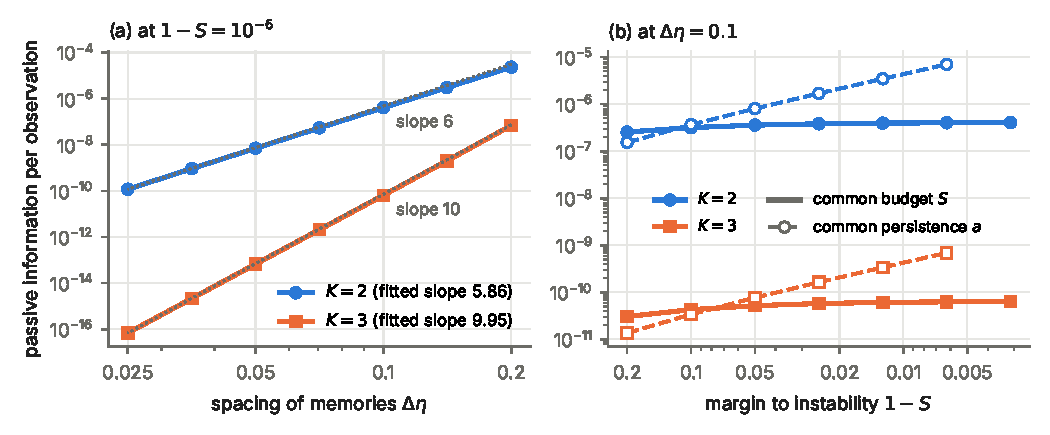
\includegraphics[width=\textwidth]{fig_barrier.pdf}
\caption{The passive barrier near instability. Both panels show the Gaussian Kullback--Leibler information per observation between the stationary price processes of two populations whose merged measures are the $K$-node Gauss and Gauss--Radau rules on memories spread over $\Delta\eta$ around $0.5$ (total weight $0.3$, impact $\kappa=0.5$). (a)~At a common feedback budget one millionth below instability, the information falls like $(\Delta\eta)^{4K-2}$ (dotted lines). (b)~Held at a common budget (solid), the information stays bounded as the margin $1-S$ shrinks; held at a common persistence (dashed), it grows without bound, because the budgets then differ. Computed from the closed-form spectra; scripts in \nolinkurl{research_extension/fragility_reveals/}.}
\label{n:fig_barrier}
\end{figure}

\paragraph{How large is the barrier?} Table~\ref{n:tab_cal} puts numbers on part~(iii) for two groups. What matters is the spread of memories relative to their size. Populations whose memories all have half-lives between 5 and 9 days cannot be told apart with both error probabilities at $5\%$ from less than $4{,}000$ years of daily prices, however close the market is to instability. When half-lives differ by a factor of three or more, a century of daily data can suffice. With three groups the numbers grow to the order of $10^8$ years. The numbers bound every test, for the passive record; probing faces the same order (part~(i)). The exponents do not depend on Gaussian noise: with real Bitcoin price noise injected into synthetic groups, the fitted slopes are $-6.01$ and $-9.81$, against $-6$ and $-10$ (Supplement Section~\ref{sec:injection}).

\begin{table}[t]
\centering
\caption{Years of daily price data below which no test tells the two populations of Theorem~\ref{n:cost}(i) apart with both error probabilities at $5\%$.}
\label{n:tab_cal}
\begin{tabular}{cccrr}
\toprule
& memory rates & half-lives (days) & $1-S=0.1$ & $1-S=10^{-6}$\\
\midrule
$K=2$ & $0.5\pm0.1$ & 0.8--1.4 & 20{,}000 & 16{,}000\\
& $0.5\pm0.05$ & 0.9--1.2 & $1.2\times10^{6}$ & $9.0\times10^{5}$\\
& $0.8\pm0.1$ & 1.9--6.6 & 100 & 69\\
& $0.8\pm0.05$ & 2.4--4.3 & 6{,}000 & 3{,}900\\
& $0.9\pm0.05$ & 4.3--13.5 & 120 & 77\\
& $0.9\pm0.025$ & 5.2--8.9 & 7{,}000 & 4{,}300\\
\midrule
$K=3$ & $0.5\pm0.1$ & 0.8--1.4 & $1.5\times10^{8}$ & $9.9\times10^{7}$\\
& $0.5\pm0.05$ & 0.9--1.2 & $1.5\times10^{11}$ & $9.6\times10^{10}$\\
\bottomrule
\end{tabular}
\par\smallskip
\parbox{\textwidth}{\footnotesize Bound: $n\ge\ln 5/\mathrm{KL}$ observations (Bretagnolle--Huber), with KL the Gaussian information per observation, computed as in Figure~\ref{n:fig_barrier}, at a common feedback budget $S$, impact $\kappa=0.5$ and feedback share $\kappa\sum_iq_i=0.3$ (total weight $0.6(1-r_c)$ at centre rate $r_c$). Memory rates are per day, 252 days a year; for traders whose memories are counted in five-minute periods, with prices recorded every five minutes around the clock, divide by $417$. Two significant digits. Script: \nolinkurl{research_extension/fragility_reveals/calibration_table.py}.}
\end{table}

\section{Who needs composition, and what disclosure buys}\label{n:sup}

\begin{proposition}[Market-wide versus targeted action]\label{n:target}
Let $q_i\ge0$, let the market be stable with $(a,\kappa)$ known, and let a supervisor need the feedback budget below a ceiling $\bar s$, with $a<\bar s<1$.
\begin{enumerate}[label=(\roman*),itemsep=1pt]
\item \emph{Market-wide.} Scaling all feedback activity by $\theta$ meets the ceiling exactly when $a+\theta(S-a)\le\bar s$. This depends on the population only through $S$, and so only through the kernel.
\item \emph{Targeted.} Halting the largest group does not. For every $K\ge2$ there are two populations whose merged measures have the same moments of order $0,\ldots,2K-2$, so that their budgets differ only by order $(\Delta\eta)^{2K-1}$, while their largest groups differ by a fixed amount, so that for a range of ceilings the halt meets the ceiling in one and not the other. Making this decision from $N$ reset records with both errors at most $1/4$ needs $N\ge c\,\sigma^2(\Delta\eta)^{-(4K-2)}$.
\end{enumerate}
\end{proposition}

Part~(i) is Supplement Proposition~\ref{prop:target}(i). Part~(ii) is Supplement Proposition~\ref{prop:targetK}; its pair comes from a family of quadrature rules whose weights are the values of one function at their nodes (Supplement Lemma~\ref{lem:everyK}).

\begin{theorem}[Value of class-tagged disclosure]\label{n:disc}
Suppose that, in addition to prices, the observer receives each class's flow with Gaussian measurement noise. On the rich class of Theorem~\ref{n:cost}(ii), the number of experiments needed to recover the weights falls from order $(\Delta\eta)^{-(4K-2)}$ to a bound that does not depend on $\Delta\eta$. For the rates it falls to order $(\Delta\eta)^{-2}$.
\end{theorem}

This is Supplement Theorem~\ref{thm:discvalue}; Supplement Proposition~\ref{prop:tagged} gives the regression that achieves it, one class at a time, with a variance that depends only on that class. Supplement Proposition~\ref{prop:choice} says when a supervisor should pay for such an audit trail: when the algorithms to be told apart are close enough that prices take too long, but not so close that even tagged data cannot help, and when the trail covers enough markets to recover its fixed cost.

Real regimes tag some traders and leave the rest anonymous. The next result prices that.

\begin{theorem}[Partial disclosure]\label{n:partial}
If the flows of $m$ of the $K$ groups are tagged, the cost of composition is that of the $K'=K-m$ untagged groups alone: of order $(\Delta\eta)^{-(4K'-2)}$ experiments if $K'\ge2$, and a number that does not depend on $\Delta\eta$ if $K'\le1$.
\end{theorem}

This is Supplement Theorem~\ref{thm:partial}; the lower bound uses the $K'$-node Gauss and Gauss--Radau pair with the tagged groups held fixed, and the upper bound subtracts the tagged groups' estimated contribution and applies Prony's method to the rest. Each tag lowers the exponent by four. The tag that leaves a single group untagged is worth the most, a factor of order $(\Delta\eta)^{-6}$, and the last tag is worth nothing for the weights. So a supervisor never needs to tag everyone: tagging all but one memory class gives the full composition at a cost that does not depend on how close the memories are. What matters is how many distinct memory classes stay untagged, not how many traders. A regime that tags registered high-speed traders gets the full benefit only if everyone else behaves, in memory, like a single class.

A supervisor who sees several markets has a second route that needs no tags at all. An algorithm's memory, its lookback, is the same in every market it trades, while its participation varies from market to market.

\begin{theorem}[Pooling markets]\label{n:pool}
Let the same $K$ algorithms trade in $D$ markets, with common memory rates and market-specific weights whose matrix has rank $D\le K$. Pooling the price records of the $D$ markets, the data needed to learn composition are of order $(\Delta\eta)^{-2(K-1+\lceil K/D\rceil)}$ near generic configurations: $(\Delta\eta)^{-(4K-2)}$ with one market and $(\Delta\eta)^{-2K}$ with $K$ or more. Over a compact class the exponent lies between $2(K-1+\lceil K/D\rceil)$ and $4K-2$, so pooling never needs more data than one market; whether it equals the local exponent is a global question that is open in general.
\end{theorem}

This is Supplement Theorem~\ref{thm:pool}. The lower bound on the joint records of all markets is machine-checked for any matched pair; the rank condition behind the matching upper bound is verified exactly for up to eight algorithms, and Monte Carlo runs of the estimator reproduce the predicted rates. Cross-market surveillance is a partial substitute for tagging, and the converse constrains hiding: to stay as hidden as in a single market, the algorithms must trade in the same proportions everywhere. For two algorithms with half-lives between 5 and 9 days, about $7{,}000$ years of daily prices in one market become at least about $90$ in two markets in which their shares differ by $50$ percentage points (hardest pair found numerically; Supplement Section~\ref{sec:pool}).

Two further results say what the supervisor cannot use instead. Markets with the same eigenvalues, the same one-step and long-run price variance can have arbitrarily different worst-case short-run gains, so no monitor built on eigenvalues and second moments of prices is uniformly safe (Supplement Theorem~\ref{thm:blind}). And what prices hide is economically specific: for desks that track a trend with Kalman filters, prices depend on the desks only through their signal-to-noise ratios and intensities, so how good each desk's information is, the thing a supervisor would most like to know, is what costs $(\Delta\eta)^{-(4K-2)}$ to learn (Supplement Propositions~\ref{prop:primitives} and~\ref{prop:tied}).

The results so far take the groups' rules as given. A group that expects to be targeted has a reason to change them.

\begin{proposition}[Hiding caps targeting]\label{n:hiding}
A supervisor observes prices, under any probes and for any record length, and then targets a given group or not. Being targeted costs the group $P>0$. Suppose the group can adopt, at private cost $C_0$, a rule that gives the population the kernel of a population that the supervisor targets with probability $\alpha$. Then in any best response the group is targeted with probability at most $\alpha+C_0/P$, whatever the probes, record length and decision rule.
\end{proposition}

The proof is two lines from Theorem~\ref{n:suff} (Supplement Proposition~\ref{prop:hiding}). More data make the group's original rule easier to detect and so make hiding more attractive. With several groups, the bound applies to each group's best response given the others' rules, so it holds group by group in any equilibrium; what determines each group's $\alpha$ is not modelled. A class tag is attached to the account, so changing the trading rule does not remove it.

\section{Position limits: calm hides, stress reveals}\label{n:sat}

Real feedback traders have position limits. Let trader $i$ have memory rate $r_i$, capacity $c_i>0$ and leverage $\ell_i$, and trade $c_i\psi(\ell_im_{i,t})$, where $m_{i,t}$ is its exponentially weighted signal and $\psi$ is a shape common to all traders. The leading case is the hard limit $\psi(u)=\max(-1,\min(1,u))$: inside its band a trader is linear with weight $c_i\ell_i$; at the edge its position is capped. Write $\nu=\sum_ic_i\delta_{(r_i,\ell_i)}$ for the capacity measure on memory and leverage.

\begin{theorem}[Two layers]\label{n:sat_thm}
\begin{enumerate}[label=(\roman*),itemsep=1pt]
\item \emph{Sufficiency.} For any shape, populations with the same $\nu$ give the same prices, profits and equilibria. The kernel is one linear functional of $\nu$, $k_m=\int r^m\ell\,d\nu$, and does not determine it.
\item \emph{Calm hides.} Under hard limits, two populations with the same kernel give identical price and order-flow paths until some trader first reaches its limit. Any record of the market before date $T$ distinguishes them with total-variation distance at most the probability that a limit is reached before $T$. With Gaussian news and no probe this is at most $T(n+n')e^{-1/(2\vartheta^2)}$ for the $n+n'$ traders of the two populations, where $\vartheta$ is the largest standard deviation of a trader's position relative to its limit.
\item \emph{Stress reveals.} If every trader has $r_i\ge0$ and $\ell_i\ne0$ and responses are observed exactly, probes of all sizes identify the signed capacity measure $\tilde\mu=\sum_ic_i\,\mathrm{sgn}(\ell_i)\,\delta_{(r_i,|\ell_i|)}$, and nothing finer, for the hard limit and for $\tanh$. For $\tanh$, probes in any neighbourhood of zero suffice. For a cubic shape the result fails.
\end{enumerate}
\end{theorem}

Parts (i)--(iii) are Supplement Theorems~\ref{thm:satsuff}, \ref{thm:stress} and~\ref{thm:satident}; for the hard limit and for $\tanh$ with probes of all sizes, part~(iii) is machine-checked for any number of traders; the small-probe statement is proved on paper. The theorem assumes exactly observed responses; with observation noise, a minimum-distance estimator recovers the signed measure consistently, without a rate (Supplement Proposition~\ref{prop:noisystress}). Its last step, for $\tanh$, is the uniqueness of one-hidden-layer networks up to sign flips \citep{sussmann1992}, which is why only the signed measure is identified. What the market adds is the reduction: probing recovers the flow map from prices, and two price dates give different memory--leverage pairs different scales.

The economic content is in part~(ii). How close traders are to their limits, which governs behaviour in a crash, leaves no trace in calm prices. It can be learned only by pushing traders toward their limits or from disclosure.

\section{Scope and conclusion}\label{n:concl}

\paragraph{Evidence.} The contribution is theoretical, and the tagged flows and position limits it concerns are rarely observed. We ran two registered tests on the closest public data, each run once, with the wording of the result fixed in advance; Supplement Section~\ref{sec:scope} reports both in full. In a pre-registered out-of-sample test on Taiwan's tagged exchange flows (2019--2023), prices improve forecasts of foreign investors' flow as the registered criterion requires, but a pre-specified check attributes the gain to prices revealing past flow rather than to feedback. We do not claim that tagged flow in Taiwan responds to price deviations. The registered test is supportive, but its pre-specified diagnostic attributes the gain to reverse causality. The Binance test was specified after its sample period, before its data were read. A pre-specified test on Binance perpetual futures was inconclusive (calm difference $-0.002$, 90\% interval $[-0.007, 0.004]$; difference-in-differences $0.041$, $p=0.553$). It neither supports nor contradicts the prediction of Section~\ref{n:sat}.

The sufficiency results hold whenever aggregate feedback flow is a causal function of public signals; the kernel is the sufficient object when that function is linear, and $\nu$ when it saturates as in Section~\ref{n:sat}. The explicit identification and cost results need linear rules with exponential memory. For general rules, prices identify the aggregate flow map and the lower bounds still hold (Supplement Theorem~\ref{thm:anypop}), but no upper bound is proved, and for some families composition is not identified at all. For linear rules with general completely monotone memory the minimax accuracy is of order $1/\log(N/\sigma^2)$ (Supplement Theorem~\ref{thm:general}). Simulations of saturating, adaptive and neural trading rules show where the linear theory holds and where it fails (Supplement Section~\ref{sec:learners}). The passive results assume Gaussian news. Traders who change their rules as they learn are outside the theorems, apart from Proposition~\ref{n:hiding}.

\paragraph{The problem this leaves.} Together the results pose a problem. A supervisor who must keep a market stable cannot learn who trades in it from prices, at any reasonable cost, in calm conditions or near a crash; the traders can hide if it tries; and the information that would identify them arrives, if at all, only when limits are already being hit. Whether a market can be kept safe without that knowledge, using only what prices do reveal, is the question taken up in the companion paper \citep{niroula2026b}.

\paragraph{What this says about the rules.} The results sort the regulatory choices above. A market-wide measure, such as a uniform limit on feedback activity or a pause triggered by the feedback budget, needs no identification and can be set from prices. A measure aimed at particular algorithms cannot be set from prices at any reasonable cost, and the targeted algorithms can make it harder still by imitating others. It needs flow tagged by class or account, which is what the Chinese, Indian, Japanese and European regimes collect. Whether that data make the targeted measures worth their cost is an empirical question that only those tags can answer.

Within these limits the message is simple. Prices tell a supervisor the kernel and nothing more, and the kernel is enough for any action that treats the market as a whole. Actions aimed at one group need composition, which prices supply only at a steep and known price and which a group can hide at a bounded cost. Disclosure tagged by trader class removes that price. The same split recurs with position limits: calm markets reveal the kernel, and only stress or disclosure reveals how close traders are to their limits.

\subsection*{Declarations}

\paragraph{Author contributions.} Pratik Niroula: conceptualization, methodology, formal analysis, software, investigation, data curation, writing (original draft). Prashant Niroula: validation (verification of the proofs, the Lean~4 formalizations and the empirical calculations), writing (review and editing). Sujan Khatiwada: validation (verification of the proofs, the Lean~4 formalizations and the empirical calculations), writing (review and editing). All authors approved the final manuscript.

\paragraph{Funding.} This research received no external funding.

\paragraph{Competing interests.} The authors declare no competing interests.

\paragraph{Data availability.} All data are public. The Taiwan test uses the Taiwan Stock Exchange's daily reports of trading by the three major institutional investors (T86), closing quotes (MI\_INDEX), ex-rights and ex-dividend adjustments (TWT49U) and market totals (FMTQIK), from \url{https://www.twse.com.tw}. The Binance test uses daily files of five-minute candles and trading metrics (including open interest) for USD-margined perpetual futures from the Binance public data archive (\url{https://data.binance.vision}). The registered specifications, amendments, executors, notebooks, result files and test-unlock counters are in the public repository.

\paragraph{Code availability.} All code, Lean~4 proofs and result files are public at \url{https://github.com/Pratikn03/Fianince}.

\paragraph{Ethics approval.} Not applicable. The study uses only public market data and involves no human participants or personal data.

\paragraph{Declaration of generative AI and AI-assisted technologies.} During the preparation of this work the authors used Claude, ChatGPT/Codex and Gemini for research development, code, numerical checks, Lean proofs, drafting and internal critique, as stated on the title page. After using these tools, the authors reviewed and edited the content as needed and take full responsibility for the content of the publication.


\begin{thebibliography}{99}\setlength{\itemsep}{2pt}\small
\bibitem[Albertini and Sontag(1993)]{albertini1993} Albertini, F., and E.~D. Sontag (1993). For neural networks, function determines form. \emph{Neural Networks} 6, 975--990.
\bibitem[Auclert et~al.(2024)]{auclert2024} Auclert, A., M. Rognlie, and L. Straub (2024). The intertemporal Keynesian cross. \emph{Journal of Political Economy} 132, 4068--4121.
\bibitem[Barberis et~al.(2015)]{barberis2015} Barberis, N., R. Greenwood, L. Jin, and A. Shleifer (2015). X-CAPM: An extrapolative capital asset pricing model. \emph{Journal of Financial Economics} 115, 1--24.
\bibitem[Barberis et~al.(2018)]{barberis2018} Barberis, N., R. Greenwood, L. Jin, and A. Shleifer (2018). Extrapolation and bubbles. \emph{Journal of Financial Economics} 129, 203--227.
\bibitem[Barroso et~al.(2022)]{barroso2022} Barroso, P., R.~M. Edelen, and P. Karehnke (2022). Crowding and tail risk in momentum returns. \emph{Journal of Financial and Quantitative Analysis} 57, 1313--1342.
\bibitem[Batenkov et~al.(2021)]{batenkov2021} Batenkov, D., G. Goldman, and Y. Yomdin (2021). Super-resolution of near-colliding point sources. \emph{Information and Inference} 10, 515--572.
\bibitem[Bernstein(1914)]{bernstein1914} Bernstein, S. (1914). Sur la meilleure approximation de $|x|$ par des polyn\^omes de degr\'es donn\'es. \emph{Acta Mathematica} 37, 1--57.
\bibitem[Brock and Hommes(1998)]{brock1998} Brock, W.~A., and C.~H. Hommes (1998). Heterogeneous beliefs and routes to chaos in a simple asset pricing model. \emph{Journal of Economic Dynamics and Control} 22, 1235--1274.
\bibitem[Brunnermeier and Pedersen(2009)]{brunnermeier2009} Brunnermeier, M. K., and L. H. Pedersen (2009). Market liquidity and funding liquidity. \emph{Review of Financial Studies} 22, 2201--2238.
\bibitem[Cagan(1956)]{cagan1956} Cagan, P. (1956). The monetary dynamics of hyperinflation. In M. Friedman (Ed.), \emph{Studies in the Quantity Theory of Money}, 25--117. University of Chicago Press.
\bibitem[Celov et~al.(2010)]{celov2008} Celov, D., R. Leipus, and A. Philippe (2010). Asymptotic normality of the mixture density estimator in a disaggregation scheme. \emph{Journal of Nonparametric Statistics} 22, 425--442.
\bibitem[De Long et~al.(1990)]{delong1990} De Long, J. B., A. Shleifer, L. H. Summers, and R. J. Waldmann (1990). Positive feedback investment strategies and destabilizing rational speculation. \emph{Journal of Finance} 45, 379--395.
\bibitem[Dreesen et~al.(2017)]{dreesen2017} Dreesen, P., D.~T. Westwick, J. Schoukens, and M. Ishteva (2017). Modeling parallel Wiener--Hammerstein systems using tensor decomposition of Volterra kernels. In \emph{Latent Variable Analysis and Signal Separation (LVA/ICA 2017)}, Lecture Notes in Computer Science 10169, 16--25. Springer.
\bibitem[Fan(1991)]{fan1991} Fan, J. (1991). On the optimal rates of convergence for nonparametric deconvolution problems. \emph{Annals of Statistics} 19, 1257--1272.
\bibitem[Fefferman(1994)]{fefferman1994} Fefferman, C. (1994). Reconstructing a neural net from its output. \emph{Revista Matem\'atica Iberoamericana} 10, 507--555.
\bibitem[Forni and Lippi(1997)]{forni1997} Forni, M., and M. Lippi (1997). \emph{Aggregation and the Microfoundations of Dynamic Macroeconomics}. Oxford University Press.
\bibitem[Granger(1980)]{granger1980} Granger, C. W. J. (1980). Long memory relationships and the aggregation of dynamic models. \emph{Journal of Econometrics} 14, 227--238.
\bibitem[Grossman and Miller(1988)]{grossman1988} Grossman, S. J., and M. H. Miller (1988). Liquidity and market structure. \emph{Journal of Finance} 43, 617--633.
\bibitem[Heinrich and Kahn(2018)]{heinrich2018} Heinrich, P., and J. Kahn (2018). Strong identifiability and optimal minimax rates for finite mixture estimation. \emph{Annals of Statistics} 46, 2844--2870.
\bibitem[Ho and Stoll(1981)]{hostoll1981} Ho, T., and H. R. Stoll (1981). Optimal dealer pricing under transactions and return uncertainty. \emph{Journal of Financial Economics} 9, 47--73.
\bibitem[Katz et~al.(2023)]{katz2023} Katz, R., N. Diab, and D. Batenkov (2023). On the accuracy of Prony's method for recovery of exponential sums with closely spaced exponents. arXiv preprint arXiv:2302.05883.
\bibitem[Kong and Valiant(2017)]{kong2017} Kong, W., and G. Valiant (2017). Spectrum estimation from samples. \emph{Annals of Statistics} 45, 2218--2247.
\bibitem[Koyck(1954)]{koyck1954} Koyck, L.~M. (1954). \emph{Distributed Lags and Investment Analysis}. North-Holland.
\bibitem[Kyle(1985)]{kyle1985} Kyle, A. S. (1985). Continuous auctions and insider trading. \emph{Econometrica} 53, 1315--1335.
\bibitem[Lecl\`ere and Rosenbaum(2026)]{leclere2026} Lecl\`ere, J., and M. Rosenbaum (2026). Mean-field equilibrium of heterogeneous agents under market impact. arXiv preprint arXiv:2609.03115.
\bibitem[Li et~al.(2022)]{li2022} Li, W., Z. Zhu, W. Gao, and W. Liao (2022). Stability and super-resolution of MUSIC and ESPRIT for multi-snapshot spectral estimation. \emph{IEEE Transactions on Signal Processing} 70, doi:10.1109/TSP.2022.3204454.
\bibitem[Moitra(2015)]{moitra2015} Moitra, A. (2015). Super-resolution, extremal functions and the condition number of Vandermonde matrices. In \emph{Proceedings of the 47th Annual ACM Symposium on Theory of Computing (STOC)}, 821--830.
\bibitem[Muth(1960)]{muth1960} Muth, J.~F. (1960). Optimal properties of exponentially weighted forecasts. \emph{Journal of the American Statistical Association} 55, 299--306.
\bibitem[Nerlove(1958)]{nerlove1958} Nerlove, M. (1958). Adaptive expectations and cobweb phenomena. \emph{Quarterly Journal of Economics} 72, 227--240.
\bibitem[Niroula et~al.(2026b)]{niroula2026b} Niroula, P., S. Alkhushayni, Y. Chen, M. Bhavsar, and P. Niroula (2026). From human markets to machine markets: Transient amplification, an exact depth condition, and a maximal pre-trade guard. Working paper, Minnesota State University, Mankato.
\bibitem[Pesaran and Chudik(2014)]{pesaran2014} Pesaran, M.~H., and A. Chudik (2014). Aggregation in large dynamic panels. \emph{Journal of Econometrics} 178, 273--285.
\bibitem[Rivlin(1981)]{rivlin1981} Rivlin, T. J. (1981). \emph{An Introduction to the Approximation of Functions}. Dover.
\bibitem[Sargent(1976)]{sargent1976} Sargent, T.~J. (1976). The observational equivalence of natural and unnatural rate theories of macroeconomics. \emph{Journal of Political Economy} 84, 631--640.
\bibitem[Sussmann(1992)]{sussmann1992} Sussmann, H.~J. (1992). Uniqueness of the weights for minimal feedforward nets with a given input-output map. \emph{Neural Networks} 5, 589--593.
\bibitem[Tsybakov(2009)]{tsybakov2009} Tsybakov, A. B. (2009). \emph{Introduction to Nonparametric Estimation}. Springer.
\bibitem[Varga and Carpenter(1985)]{varga1985} Varga, R. S., and A. J. Carpenter (1985). On the Bernstein conjecture in approximation theory. \emph{Constructive Approximation} 1, 333--348.
\bibitem[Vla\v{c}i\'c and B\"olcskei(2022)]{vlacic2019} Vla\v{c}i\'c, V., and H. B\"olcskei (2022). Neural network identifiability for a family of sigmoidal nonlinearities. \emph{Constructive Approximation} 55, 173--224.
\bibitem[Wu and Yang(2020)]{wu2020} Wu, Y., and P. Yang (2020). Optimal estimation of Gaussian mixtures via denoised method of moments. \emph{Annals of Statistics} 48, 1981--2007.
\bibitem[Zaffaroni(2004)]{zaffaroni2004} Zaffaroni, P. (2004). Contemporaneous aggregation of linear dynamic models in large economies. \emph{Journal of Econometrics} 120, 75--102.
\bibitem[Boswijk et~al.(2007)]{boswijk2007} Boswijk, H.~P., C.~H. Hommes, and S. Manzan (2007). Behavioral heterogeneity in stock prices. \emph{Journal of Economic Dynamics and Control} 31, 1938--1970.

\bibitem[Franke and Westerhoff(2012)]{franke2012} Franke, R., and F. Westerhoff (2012). Structural stochastic volatility in asset pricing dynamics: Estimation and model contest. \emph{Journal of Economic Dynamics and Control} 36, 1193--1211.

\bibitem[Hommes(2006)]{hommes2006} Hommes, C.~H. (2006). Heterogeneous agent models in economics and finance. In L. Tesfatsion and K.~L. Judd (eds.), \emph{Handbook of Computational Economics}, Vol.~2, 1109--1186. Elsevier.

\bibitem[Lux and Zwinkels(2018)]{lux2018} Lux, T., and R.~C.~J. Zwinkels (2018). Empirical validation of agent-based models. In C. Hommes and B. LeBaron (eds.), \emph{Handbook of Computational Economics}, Vol.~4, 437--488. Elsevier.

\bibitem[Niroula et~al.(2026a)]{niroula2026a} Niroula, P., P. Niroula, and S. Khatiwada (2026a). What prices cannot tell a market supervisor: The cost of identifying trader groups and the value of class disclosure. Working paper, 5 November 2026, \url{https://github.com/Pratikn03/Fianince}.

\end{thebibliography}
\appendix
\clearpage
\singlespacing\small\sloppy
\renewcommand{\topfraction}{0.9}\renewcommand{\bottomfraction}{0.8}\renewcommand{\textfraction}{0.07}\renewcommand{\floatpagefraction}{0.75}
\setcounter{page}{1}\renewcommand{\thepage}{S-\arabic{page}}\renewcommand{\thesection}{S\arabic{section}}\setcounter{table}{0}\renewcommand{\thetable}{S\arabic{table}}\setcounter{figure}{0}\renewcommand{\thefigure}{S\arabic{figure}}
\begin{center}{\Large Online Supplement}\\[4pt]{\large Observationally Equivalent Algorithms}\\[2pt]{\normalsize Niroula, Niroula and Khatiwada, 12 November 2026}\end{center}

\noindent Sections~S1--S7 state every result in full, with the remarks, machine-check notes and the results that the main text omits. The remaining sections give the proofs, further results, machine checks and notation. Theorem numbers in the supplement are those of these sections, not of the main text. The main text's results correspond to them as follows: Theorem~\ref{n:suff} to Theorem~\ref{thm:eqinv} and Proposition~\ref{prop:anylinear}; Theorem~\ref{n:ident} to Theorem~\ref{thm:merged}(i); Theorem~\ref{n:cost} to Theorems~\ref{thm:kcohort}, \ref{prop:esprit} and~\ref{prop:passive}; Proposition~\ref{n:target} to Propositions~\ref{prop:target}(i) and~\ref{prop:targetK}; Theorem~\ref{n:disc} to Theorem~\ref{thm:discvalue}; Proposition~\ref{n:nearcrit} to Proposition~\ref{prop:nearcrit}; Proposition~\ref{n:hiding} to Proposition~\ref{prop:hiding}; Theorem~\ref{n:partial} to Theorem~\ref{thm:partial}; Theorem~\ref{n:pool} to Theorem~\ref{thm:pool}; Theorem~\ref{n:sat_thm} to Theorems~\ref{thm:satsuff}, \ref{thm:stress} and~\ref{thm:satident}.

\section{Model and motivating examples}\label{sec:model}

Time is discrete. Let $p_t$ be the price, $p^*$ the fundamental value and $x_t=p_t-p^*$ the pricing error. A reduced-form dealer sector absorbs net order flow with price impact $\kappa>0$, an imposed primitive rather than an equilibrium quote, and arbitrage pulls the error toward zero with persistence $a\in[0,1)$:
\begin{equation}\label{eq:price}
x_t = a x_{t-1} + \kappa \sum_{i=1}^K q_i y_{i,t-1} + \kappa v_t + \varepsilon_t,
\end{equation}
where $v_t$ is an executed probe quantity and $\varepsilon_t$ a price innovation (news). Group $i$ holds a state $y_{i,t}$ with exponential memory and trades $q_i y_{i,t}$:
\begin{equation}\label{eq:cohort}
y_{i,t} = (1-\eta_i)\,y_{i,t-1} + \eta_i x_t,\qquad \eta_i\in(0,1).
\end{equation}
The ordering is \emph{price first}: the price responds to the probe, then groups update. Write $r_i=1-\eta_i$ for the memory rate and $w_i=q_i\eta_i$ for the merged weight. The feedback kernel and its transform are
\begin{equation}\label{eq:kernel}
k_m=\sum_i w_i r_i^{\,m},\qquad G(z)=\sum_i \frac{w_i z}{z-r_i},
\end{equation}
and the transfer function from probes to prices, $H(z)=\sum_{j\ge0}h_jz^{-j}$, is
\begin{equation}\label{eq:H}
H(z)=\frac{\kappa z}{z-a-\kappa G(z)}=\frac{\kappa zD(z)}{(z-a)D(z)-\kappa N(z)},\qquad G=\frac ND,\quad D(z)=\prod_{i}(z-r_i),
\end{equation}
with impulse response $h_0=H(\infty)=\kappa,h_1,h_2,\ldots$; in particular $H(1)=\sum_jh_j=\kappa/(1-S)$, where $S=a+\kappa\sum_iq_i$ is the feedback budget. Stacking $z_t=(x_t,y_{1,t},\ldots,y_{K,t})^\top$ gives $z_t=Jz_{t-1}+bv_t$, where, because groups update on the same period's price, the probe enters every state on impact through
\begin{equation}\label{eq:b}
b=\kappa\,(1,\eta_1,\ldots,\eta_K)^\top ,
\end{equation}
and
\begin{equation}\label{eq:J}
J=\begin{pmatrix} a & \kappa q_1 & \cdots & \kappa q_K\\ \eta_1 a & 1-\eta_1+\eta_1\kappa q_1 & \cdots & \eta_1\kappa q_K\\ \vdots & & \ddots & \vdots\\ \eta_K a & \eta_K\kappa q_1 & \cdots & 1-\eta_K+\eta_K\kappa q_K\end{pmatrix},\qquad S\equiv a+\kappa\sum_i q_i .
\end{equation}
In the \emph{positive economy} ($q_i\ge0$), $J$ is entrywise nonnegative, its price row sums to $S$, and the economy is Schur stable iff $S<1$.

\begin{lemma}[Two motivating examples: filtering and learning]\label{lem:micro}
\begin{enumerate}[label=(\roman*)]
\item \emph{Kalman memory.} A desk that tracks a latent random-walk trend $v_{t+1}=v_t+\zeta_{t+1}$, $\zeta\sim N(0,\sigma_\zeta^2)$, from signals $r_t=v_t+\nu_t$, $\nu\sim N(0,\sigma_\nu^2)$, using the steady-state Kalman filter, updates as $\hat v_{t+1}=(1-\eta)\hat v_t+\eta r_t$ with
\begin{equation}\label{eq:kgain}
\eta=\frac{-\sigma_\zeta^2+\sqrt{\sigma_\zeta^4+4\sigma_\zeta^2\sigma_\nu^2}}{2\sigma_\nu^2}\in(0,1).
\end{equation}
\item \emph{Gradient memory.} Online gradient descent with $L_2$ regularization $\gamma\in(0,1)$, step size $\alpha>0$ and loss $\tfrac12H(x_t-\theta_t)^2$ gives $\theta_{t+1}=(1-\eta)\theta_t+\eta q x_t$ with $\eta=\gamma+\alpha H\in(0,1)$ and $q=\alpha H/\eta$. A tabular value update with learning rate $\eta$ at a fixed state has the same form; general reinforcement-learning policies need not.
\end{enumerate}
\end{lemma}

\paragraph{Why exponential memory, and what is assumed.} Exponential memory is the oldest model of expectations in economics: adaptive expectations \citep{cagan1956,nerlove1958} and geometric distributed lags \citep{koyck1954}, and \citet{muth1960} showed that exponentially weighted forecasts are optimal for a random walk observed with noise, which is Lemma~\ref{lem:micro}(i). Lemma~\ref{lem:micro} shows that two different design philosophies, Bayesian filtering and regularized online learning, produce the same reduced-form state. A third example is a desk that each period trades the amount that maximizes $\hat v_tu-\tfrac12(\kappa+\lambda)u^2$, a one-period trade-off between its trend forecast $\hat v_t$ and quadratic impact and holding costs. Its trade is $u_t=\hat v_t/(\kappa+\lambda)$. If the forecast is updated exponentially, $\hat v_{t+1}=(1-\eta)\hat v_t+\eta x_t$, the trade follows the same recursion, $u_{t+1}=(1-\eta)u_t+wx_t$ with $w=\eta/(\kappa+\lambda)$. This is a static first-order condition, not a dynamic optimum. In these families the memory rate is a known function of a tuning parameter, the desk's signal-to-noise ratio, its regularization or its cost parameters. That is the private information a supervisor would like to recover, although real algorithms need not belong to any of these families. Applied to the pricing error, a desk that cannot separate fundamental news from transitory deviations treats recent deviations as a persistent trend, which is the exponential extrapolation of \citet{barberis2015,barberis2018}. Nothing in the model says such trading is profitable.

The results use six modelling choices: linearity; price-first timing within a period; exponential memory (needed for the identification result, Theorem~\ref{thm:merged}, and the cost results of Section~\ref{sec:cost}, but not for sufficiency); algorithms that do not change their rules when observed (Proposition~\ref{prop:hiding} relaxes this for one group); known primitives $(a,\kappa)$; and stated observation contracts. Unknown primitives can only enlarge the set of candidate populations, so the lower bounds remain valid; Corollary~\ref{cor:unknown_primitives} in the supplement shows that estimating them leaves the upper-bound rate unchanged. Section~\ref{sec:equilibrium} replaces the primitive $(a,\kappa)$ by an equilibrium.

\paragraph{The observer.} The cost results are stated for one observer outside the trader groups: a supervisor, an exchange's surveillance unit or a large desk. It knows $(a,\kappa)$, the law of the observation noise and, for the $K$-group results, $K$. It can \emph{wait}, recording prices driven by natural innovations; \emph{probe}, trading a sequence $v_t$ against the groups from a reset state and recording the response; or \emph{acquire disclosure}, receiving each class's flow. Independent resets are a benchmark that no outside participant can run in a live market. We use them because they make the information content of the data exact. Reset probing is a benchmark for what can be learned, not a proposed policy. Section~\ref{sec:cost} shows separately that passive observation is no cheaper (Theorem~\ref{prop:passive}).

\section{The kernel is a sufficient statistic}\label{sec:suff}

This section states the paper's main result. In a market with an insider, noise traders, a dealer and feedback traders, all following arbitrary causal rules, the feedback traders affect every outcome only through their kernel. The notation for the insider follows \citet{kyle1985}, so in this section $x_t$ is the insider's order, not the pricing error.


\begin{theorem}[The kernel is sufficient]\label{thm:eqinv}
Consider a market with the following participants and rules.
\begin{itemize}[itemsep=1pt,topsep=2pt]
\item A value $v$ and noise trades $z_t$.
\item An insider who submits $x_t=X_t(v,\mathcal H_{t-1})$.
\item A dealer who sets $p_t=P_t(\mathcal H_{t-1},y_t)$ from the public history $\mathcal H_{t-1}$ and the total order flow $y_t=x_t+z_t+f_t$.
\item Feedback groups whose memory states update on a public price statistic $s_t=S_t(p_0,\ldots,p_t)$ by $m_{i,t+1}=r_im_{i,t}+s_t$ from $m_{i,0}=0$, with $r_i=1-\eta_i$ and aggregate flow $f_t=\sum_iw_im_{i,t}$, $w_i=q_i\eta_i$.
\end{itemize}
The rules $X$, $P$ and $S$ are arbitrary causal maps. This covers Kyle, inventory-averse, learning and misspecified dealers, and any insider strategy.
\begin{enumerate}[label=(\roman*),itemsep=1pt]
\item $f_t=\sum_{m<t}k_m\,s_{t-1-m}$, with $k_m=\sum_iw_ir_i^m$, the moments of the merged measure $M$.
\item Two group configurations produce the same aggregate flow on dates $t\le T$ for every signal sequence $(s_t)$ if and only if $k_m=k'_m$ for all $m<T$. On an unbounded horizon this holds if and only if their merged measures coincide. For a fixed signal rule $S$, the `if' direction holds for every price path. The `only if' direction needs a rule that can produce an impulse signal. It fails, for example, for $S\equiv0$, under which every configuration has zero flow.
\item If $k_m=k'_m$ for $m<T$, then for every strategy profile and every realization of $(v,z)$ the following coincide on $t\le T$: the price and order-flow paths, the insider's trades and realized profit, and the dealer's inventory. The two games therefore have the same strategy sets and the same payoff for every profile. They have the same equilibria, with the same outcomes, under any equilibrium concept defined from these payoffs and the public history.
\item Group-level quantities are not invariant. A Gauss and a Radau two-point configuration agree on $k_0,k_1,k_2$, so they are outcome-equivalent for $T=3$, while their largest groups carry weights $\tfrac12$ and $\tfrac34$.
\end{enumerate}
\end{theorem}

\paragraph{Beyond exponential memory.} The proof of part~(iii) uses only one property of the feedback traders: their aggregate flow is a fixed linear function of past public signals. So the result does not depend on exponential memory.

\begin{proposition}[Any linear population]\label{prop:anylinear}
In the market of Theorem~\ref{thm:eqinv}, replace the groups by any finite population of feedback traders $j=1,\ldots,J$ whose flows are causal linear functions of the public signal,
\[
 f_{j,t}=\sum_{m<t}\kappa^{(j)}_m\,s_{t-1-m},\qquad \kappa^{(j)}=(\kappa^{(j)}_0,\kappa^{(j)}_1,\ldots)\ \text{arbitrary real sequences},
\]
and write $k=\sum_j\kappa^{(j)}$ for the population's kernel.
\begin{enumerate}[label=(\roman*),itemsep=1pt]
\item Two populations produce the same aggregate flow on dates $t\le T$ for every signal sequence if and only if their kernels agree for $m<T$.
\item If their kernels agree for $m<T$, then for every strategy profile and every realization the price and order-flow paths, the insider's trades and realized profit, and the dealer's inventory coincide on $t\le T$, and the two games have the same equilibria under any equilibrium concept defined from payoffs and the public history.
\item Any decomposition of a kernel into individual kernels is consistent with the same outcomes. Prices, flows and all equilibrium outcomes therefore carry no information about the decomposition beyond $k$.
\end{enumerate}
\end{proposition}

\begin{proof}
(i) Aggregate flow is $f_t=\sum_{m<t}k_ms_{t-1-m}$. If the kernels agree for $m<T$, the flows agree on $t\le T$ for every signal. Conversely, the impulse signal $s_j=\mathbf 1\{j=0\}$ gives $f_{m+1}=k_m$. (ii) The strong induction in the proof of Theorem~\ref{thm:eqinv}(iii) (Supplement~\ref{app:eqinv}) uses only that $f_t$ is the same function of the signals before $t$ in both markets, which is part~(i). (iii) follows from (ii), since outcomes depend on the population only through $k$.
\end{proof}

\subsection{What prices identify}

Theorem~\ref{thm:eqinv} says that populations with the same kernel cannot be told apart by anything that price-based trading determines. The converse is that prices determine the kernel. In the probing experiment of Section~\ref{sec:model}, the response of prices to trades is a fixed function of $(a,\kappa,k)$, and it determines the merged measure.


\begin{theorem}[Merged rate--weight equivalence]\label{thm:merged}
Let $\kappa>0$ and $a\in[0,1)$ be known. Use zero initial states and a common probe contract, and observe the modeled price state $x_t$.
\begin{enumerate}[label=(\roman*)]
\item \emph{Equivalence class.} Two economies $\mathcal E^A=\{(q_i^A,\eta_i^A)\}$ and $\mathcal E^B=\{(q_j^B,\eta_j^B)\}$ produce identical price responses for every probe sequence if and only if their merged measures coincide:
\begin{equation}\label{eq:merged}
\sum_{i:\eta_i^A=\eta} q_i^A\eta \;=\; \sum_{j:\eta_j^B=\eta} q_j^B\eta\qquad\forall\eta\in(0,1].
\end{equation}
Write $a'=a+\kappa M(\{0\})$, so that groups with $\eta=1$ (rate $0$) act as part of the anchor. For $a'\neq0$ the minimal realization has dimension $1+|\mathrm{supp}(M)\cap(0,1)|$, counting distinct positive rates with nonzero merged weight after signed cancellation; for $a'=0$ the price carries no state of its own and the dimension is $|\mathrm{supp}(M)\cap(0,1)|$. A group with $\eta=1$ merges into the anchor $a$ without adding a pole.
\item \emph{Separation complexity under average power.} Consider testing a single group with rate $\bar\eta$ against two groups with rates $\bar\eta\pm\delta$ and the same total weight, on a compact family that is uniformly Schur stable with all rates in $[\epsilon,1-\epsilon]$ for some $\epsilon>0$. Observe $\tilde x_t=x_t+\nu_t$ with $\nu_t\sim N(0,\sigma_\nu^2)$ and use deterministic probes with $\frac1T\sum_{t<T}v_t^2\le P$. Any test with worst-case error at most $\alpha\in(0,1/4)$ needs
\begin{equation}\label{eq:Tpower}
T\;\ge\;\frac{4\sigma_\nu^2(1-2\alpha)^2}{C_{\mathcal F}^2P\,\delta^4}=\Omega(\delta^{-4}),
\end{equation}
where $C_{\mathcal F}$ depends only on the family, through $\epsilon$, the bound on $|H|$ implied by uniform stability, and the total weight $q$.
\end{enumerate}
\end{theorem}


The memory rates are poles of $G$ and \emph{zeros} of $H$, not closed-loop poles. This has a practical consequence verified in \citet{niroula2026a}: pole-fitting methods applied directly to the price impulse response recover closed-loop eigenvalues ($0.4256$ and $0.8224$ for $K=1$, $\eta=0.3$, $a=0.5$, $\kappa=0.8$, $q=0.2$) and miss the memory rate $0.70$.
\begin{remark}[Scope]\label{rem:scope}
The result concerns the stated model and observation contract. Groups sharing an exact rate enter prices through their merged weight; this does not determine identities or wealth allocations. Nearby rates can be distinguishable with enough information. The $\delta^{-4}$ statement in (ii) is a lower bound on a declared family, with family-dependent constants. A group may choose its rate strategically. The observer then still sees only the merged measure of the rules in use; Proposition~\ref{prop:hiding} draws the consequence.
\end{remark}
\section{Sufficiency and identification in equilibrium}\label{sec:equilibrium}

The identification results of Section~\ref{sec:suff} take the price impact $\kappa$ and the persistence $a$ of pricing errors as given. This section derives both from dealers who dislike holding inventory. It shows that the equilibrium price is the closed loop of Section~\ref{sec:model} with effective parameters and unchanged memory rates. So the kernel stays the sufficient statistic in equilibrium, and the cost of going beyond it (Section~\ref{sec:cost}) keeps its order.


\paragraph{An inventory equilibrium.}
\begin{itemize}[itemsep=1pt,topsep=2pt]
\item \emph{Fundamental and price.} The fundamental $F_t$ is a public random walk with innovation variance $\sigma_F^2$, and the price is $p_t=F_t+x_t$.
\item \emph{Groups.} They trade $u_{i,t+1}=r_iu_{i,t}+w_ix_t$, the paper's exponential memory with $w_i=q_i\eta_i$ and $r_i=1-\eta_i$.
\item \emph{Exogenous flow.} $\xi_t\sim N(0,\sigma_\xi^2)$, i.i.d., stands for noise trades or the observer's probe. Customer flow is $y_t=\sum_iu_{i,t}+\xi_t$.
\item \emph{Dealers.} Competitive dealers absorb the flow and lay off a share $1-\bar a$ of their inventory each period, so $H_t=\bar aH_{t-1}-y_t$. Each overlapping generation of dealers has CARA risk aversion $A$ and holds $H_t$ to the next date: $H_t=(E_tp_{t+1}-p_t)/(AV)$, with $V=\mathrm{Var}_t(p_{t+1})$.
\end{itemize}
We study stationary equilibria in which $x_t$ is linear in the dealers' inventory and the groups' next trades. Write $G(D)=\sum_iw_i/(D-r_i)=\int dM(r)/(D-r)$ for the Stieltjes transform of the merged measure.

\begin{theorem}[Price impact and persistence in an inventory equilibrium]\label{thm:inventory}
Consider stationary linear equilibria of the model above.
\begin{enumerate}[label=(\roman*),itemsep=1pt]
\item \emph{Characterization.} The price law
\[
 x_t=-\kappa H_t+\kappa\sum_i\frac{u_{i,t+1}}{D-r_i}
\]
with $D\ne0$ and $D\ne r_i$, is an equilibrium exactly when the induced dynamics are stable and
\begin{equation}\label{eq:inventory_eq}
 D=1-\kappa\,G(D),\qquad \kappa(D-\bar a)=A\,V\,D,\qquad V=\sigma_F^2+\frac{\kappa^2\sigma_\xi^2}{D^2}.
\end{equation}
An unexpected unit of flow moves the price by $\kappa/D$.
\item \emph{No feedback.} Then $D=1$ and the price law is exactly the paper's $x_t=\bar a\,x_{t-1}+\kappa\,y_t$. The persistence of pricing errors is the dealers' carry share, $a=\bar a$, and the impact $\kappa$ solves $\kappa(1-\bar a)=A(\sigma_F^2+\kappa^2\sigma_\xi^2)$. An equilibrium exists if and only if $\Delta=(1-\bar a)^2-4A^2\sigma_F^2\sigma_\xi^2\ge0$. When $\Delta>0$ there are two, $\kappa_\pm=\bigl((1-\bar a)\pm\sqrt\Delta\bigr)/(2A\sigma_\xi^2)$; the low-impact one $\kappa_-\approx A\sigma_F^2/(1-\bar a)$ is the price of dealer inventory risk.
\item \emph{Invariance.} The coefficients $(\kappa,D,V)$, and hence the price process, depend on the groups only through $G$, and so only through the merged measure $M$. This is Theorem~\ref{thm:eqinv} in equilibrium form.
\item \emph{Small feedback.} Let $\Delta>0$, fix $\delta>0$ with $\max_ir_i<1-\delta$, and let $\epsilon=\sup_{|D-1|\le\delta}(|G(D)|+|G'(D)|)$ be small. Then there is a unique equilibrium near $(\kappa_-,1)$. With $G(1)=\sum_iq_i$, the aggregate feedback intensity,
\[
 D=1-\kappa_-G(1)+o(\epsilon),\qquad \kappa=\kappa_-+\frac{\kappa_-^2(\bar a+2A\kappa_-\sigma_\xi^2)}{\sqrt\Delta}\,G(1)+o(\epsilon).
\]
Positive feedback raises the impact $\kappa$, and it raises the impact of an unexpected flow shock, $\kappa/D$, by more.
\end{enumerate}
\end{theorem}

\paragraph{Machine check.} See Supplement~\ref{app:mc}.

\paragraph{The identification results hold in equilibrium.} With feedback, dealers price the groups' predictable trades in advance, so the response of prices to flow is no longer the reduced form of Section~\ref{sec:model} with the primitive $(a,\kappa)$. The next theorem shows that it is still that closed loop, exactly and path by path, with new parameters and the same memory rates.

\begin{theorem}[The equilibrium is the paper's closed loop]\label{thm:eqreduced}
Take an equilibrium of Theorem~\ref{thm:inventory} with $D\ne\bar a$, and set
\[
 a^*=\frac{\bar a}{D},\qquad \kappa^*=\frac{\kappa}{D},\qquad \tilde w_i=\frac{D-\bar a}{D-r_i}\,w_i .
\]
\begin{enumerate}[label=(\roman*),itemsep=1pt]
\item \emph{Reduced form, pathwise.} Let $\tilde u_{i,t}=\frac{D-\bar a}{D-r_i}u_{i,t}$. For every realization, every initial state and every $t$,
\[
 x_t=a^*x_{t-1}+\kappa^*\Bigl(\xi_t+\sum_i\tilde u_{i,t}\Bigr),\qquad \tilde u_{i,t+1}=r_i\tilde u_{i,t}+\tilde w_ix_t .
\]
So the price follows the closed loop \eqref{eq:price}--\eqref{eq:cohort} with persistence $a^*$, impact $\kappa^*$, exogenous flow $\xi$ in place of the probe, and groups with the same memory rates and merged weights $\tilde w_i$. Its transfer function from flow to price is \eqref{eq:H} with $(a^*,\kappa^*,\tilde w)$. The equilibrium is stable if and only if this closed loop is.
\item \emph{Zeros.} For $\bar a>0$, distinct rates in $(0,1)$ and nonzero weights, the memory rates are the transmission zeros of the equilibrium price response, and none cancels (Theorem~\ref{thm:minphase}(i) with the effective parameters).
\item \emph{Boundary.} The effective merged measure is $\tilde M=h\,M$, where $h(r)=(D-\bar a)/(D-r)$ is positive. The effective parameters determine the equilibrium ones: $D=1-\kappa^*\tilde M([0,1])/(1-a^*)$, $\bar a=a^*D$ and $\kappa=\kappa^*D$. So the merged measure remains exactly what equilibrium prices identify (Theorem~\ref{thm:merged}).
\item \emph{The rates survive.} Let $(a^*,\kappa^*,W,r_c,\Delta\eta)$ satisfy the hypotheses of Theorem~\ref{thm:kcohort} with $(a,\kappa)=(a^*,\kappa^*)$. Then the two $K$-group economies of that theorem are the price responses of two inventory equilibria with identical primitives $(A,\sigma_F^2,\sigma_\xi^2,\bar a)$ and identical $(\kappa,D)$:
 \begin{itemize}[itemsep=1pt,topsep=2pt]
 \item $D=1-\kappa^*W/(1-a^*)$, which exceeds every rate;
 \item $\bar a=a^*D$ and $\kappa=\kappa^*D$;
 \item any $\sigma_F^2,\sigma_\xi^2>0$, with $A=\kappa^*D(1-a^*)/(\sigma_F^2+\kappa^{*2}\sigma_\xi^2)$;
 \item group weights $w_i=\tilde w_i(D-r_i)/(D-\bar a)>0$.
 \end{itemize}
 Hence an observer of equilibrium prices who knows the primitives needs $N\ge c\,\sigma^2(\Delta\eta)^{-(4K-2)}$ experiments. Theorem~\ref{prop:esprit} applies to the effective parameters, and the true weights follow from the effective ones by a Lipschitz map. So $N^*\asymp\sigma^2(\Delta\eta)^{-(4K-2)}$ in equilibrium.
\end{enumerate}
\end{theorem}

\paragraph{In words.} Dealers' anticipation does not hide the groups and does not move them. It replaces the persistence and impact by $\bar a/D$ and $\kappa/D$, and it rescales each group's weight by $(D-\bar a)/(D-r_i)$. Because that factor rises with $r_i$, slow-memory groups weigh more in equilibrium prices. The memory rates are untouched.
\begin{itemize}[itemsep=1pt,topsep=2pt]
\item Every result of Sections~\ref{sec:suff} and~\ref{sec:cost} that concerns the map from order flow to prices therefore holds in equilibrium: identification, sample complexity, passive observation, and probing costs computed from the price path. Its constants are evaluated at the effective parameters.
\item The lower-bound pair is not an artefact of the reduced form. Two economies with the same dealers, the same risk aversion and the same impact differ only in their groups, and they are as hard to tell apart as Theorem~\ref{thm:kcohort} says.
\item Part (i), the realization in part (iv) and the effective group recursion are machine-checked (\nolinkurl{Paper1EquilibriumReducedForm.lean}).
\item One assumption is new: the observer's probe is part of the exogenous flow that dealers price as noise. Dealers who recognized a probe would price it differently.
\end{itemize}

\paragraph{Further equilibrium results.} Four results in Supplement~\ref{app:eqinv} extend this section. None is needed for the main argument.
\begin{itemize}[itemsep=1pt,topsep=2pt]
\item \emph{A strategic insider} with short-lived information (Theorem~\ref{thm:insider}). The equilibrium is characterized in closed form and nests Kyle's one-period values. Its coefficients depend on the groups only through $G$, and the observed price is the closed loop driven through a known invertible moving-average filter. So the identification boundary and the $(\Delta\eta)^{-(4K-2)}$ rate hold with an insider present. Positive feedback raises total impact, and the insider then trades less and prices reveal less of her news.
\item \emph{Fragility} (Theorem~\ref{thm:fragility}). With positive feedback, a positive-impact equilibrium exists only if dealer risk aversion lies below a threshold. For strong feedback the threshold is inversely proportional to the feedback intensity $G(1)$. With several groups the bound depends on the population only through $G(1)$, again an aggregate.
\item \emph{Rents} (Theorem~\ref{thm:rents}). A dealer that misjudges the aggregate response by $\varepsilon$ hands an insider with a committed schedule a rent of exact order $\varepsilon$, or charges it one. Public data reveal the aggregate response at the ordinary rate. So the information that protects price formation is cheap to learn.
\item \emph{A targeted halt in equilibrium} (Theorem~\ref{thm:eqhalt}). Two markets that agree in equilibrium to within the cube of the memory spacing can differ at order one after their largest group is halted.
\end{itemize}
Disclosure keeps its value in equilibrium too (Corollary~\ref{cor:eqdisclosure}).

\section{The price of composition}\label{sec:cost}

Prices identify the kernel, and with exponential memory the kernel determines the merged measure. A finite record, however, pins down only finitely many moments of $M$, each with noise. This section asks how much data it takes to recover the groups. The answer is the known rate for finite mixtures. What the market adds is that the memories must first be extracted from a feedback loop, and that waiting is no cheaper than trading.


\subsection{Many unknown groups}

\begin{theorem}[$K$-group two-point lower bound]\label{thm:kcohort}
Fix $K\ge2$, a center $r_c\in(0,1)$, total merged weight $W>0$ and $0<\Delta\eta<\min(r_c,1-r_c)$, so that all rates lie in $(0,1)$, and assume $a+\kappa W/(1-r_c-\Delta\eta)<1$, so that every candidate economy is Schur stable. Each reset experiment observes the noisy taps $h_0,\ldots,h_{T-1}$ with $T\ge2K+1$ ($T=\infty$ allowed), so that the first tap where the two economies below differ, $h_{2K}$, is observed; the bound below uses the full response norm, which dominates any finite prefix. There exist two $K$-group economies with rates in $r_c+\Delta\eta[-1,1]$, positive weights, and merged measures whose moments of order $0,\ldots,2K-2$ coincide while the moment of order $2K-1$ differs by a constant times $(\Delta\eta)^{2K-1}$. Their impulse responses differ by $\|h^A-h^B\|_2\asymp(\Delta\eta)^{2K-1}$, so recovering the weights from $N$ independent noisy reset experiments with worst-case error probability below $1/4$ requires
\[
N\;\ge\;c\,\sigma^2(\Delta\eta)^{-(4K-2)} .
\]
The same requirement holds for the permutation-invariant loss $W_1(\hat M,M)$ between estimated and true merged measures at accuracy $c_KW\Delta\eta$, where $2c_K>0$ is the Wasserstein distance between the two normalized quadrature rules, so no relabelling of atoms escapes it.
\end{theorem}

The two losses have different targets. The weights of the two economies differ by a constant that does not shrink with $\Delta\eta$, so the first statement is about weights at fixed accuracy, which Theorem~\ref{prop:esprit} matches; the Wasserstein statement is about the memory distribution at accuracy proportional to $\Delta\eta$, which \citet{niroula2026a} match with an upper bound.

The construction uses the $K$-point Gauss and Gauss--Radau rules of the same weight function: both are positive, have $K$ atoms and integrate polynomials of degree $2K-2$ exactly. For $K=2$ it reproduces the order of Theorem~\ref{thm:twocohort}. Numerically, their low moments agree to machine precision and their moment of order $2K-1$ differs by $0.222$, $0.0533$ and $0.0131$ for $K=2,3,4$. The shrinking gap explains why constants deteriorate with $K$ on top of the exponent. The two rules also differ in their largest weight for every $K$ we checked: for $K=2,\ldots,200$ the largest Gauss--Radau weight exceeds the largest Gauss weight, by $0.25$ at $K=2$ and by about $0.79/K^2$ for large $K$ (\nolinkurl{equilibrium/gauss_radau_maxweight.py}). So the argument given for $K=2$ in Proposition~\ref{prop:target} applies to each such $K$. A proof of this comparison for every $K$ is open. The supervisory result needs less: Lemma~\ref{lem:everyK} proves that, for every $K$, some two rules of this kind have different largest weights.

\paragraph{What counts as an experiment.} In Theorem~\ref{thm:kcohort} an experiment is a unit impulse from the reset state whose response is observed with noise of variance $\sigma^2$ per tap. The exponent is the same for any probe design of bounded energy. For any probe $v$ the mean difference between the two economies is at most $\sup_\omega|\Delta\hat H(e^{i\omega})|\,\|v\|_2$, and $\sup_\omega|\Delta\hat H|=O((\Delta\eta)^{2K-1})$ because $\Delta\hat H=z^{-1}\hat H_A\hat H_B\,\Delta G$ with both responses bounded on the circle. Experiments with probe energy $E$ each therefore need $NE\gtrsim\sigma^2(\Delta\eta)^{-(4K-2)}$: a larger probe buys the same information with fewer experiments, and the account-level analysis of \citet{niroula2026a} prices the capital that a larger probe requires. The bound does not cover information obtained without trading against the groups, such as class records (Section~\ref{sec:supervision}).

\begin{theorem}[Matching upper bound for every $K$]\label{prop:esprit}
Fix $K\ge2$, a compact set $\mathcal S\subset\{s\in[-1,1]^K:s_1<\cdots<s_K\}$ of ordered rescaled rates with $\min_{i\ne j}|s_i-s_j|\ge\gamma>0$, and merged weights $w_i\in[\omega_{\min},\omega_{\max}]$ with $\omega_{\min}>0$. Consider the class of $K$-group economies with rates $r_c+\Delta\eta\,s$, $s\in\mathcal S$, and $N$ independent reset experiments, each observing at least the taps $h_0,\ldots,h_{2K}$ with Gaussian noise of variance $\sigma^2$. There are constants $c_0,C>0$ depending only on $(K,\mathcal S,\gamma,\omega_{\min},\omega_{\max},a,\kappa,r_c)$ such that, whenever $\epsilon_N\equiv\sigma N^{-1/2}(\Delta\eta)^{-(2K-1)}\le c_0/\sqrt{\log(4K/\beta)}$, Prony's method applied to the first $2K$ estimated kernel values, with its output atoms listed in increasing order of rate, recovers the weights with
\[
\max_i|\hat w_i-w_i|\;\le\;C\sqrt{\log(4K/\beta)}\;\epsilon_N
\]
with probability at least $1-\beta$. Hence $N=C'\sigma^2(\Delta\eta)^{-(4K-2)}$ experiments suffice for any fixed accuracy and confidence. On any such class that contains the Gauss and Gauss--Radau pair of Theorem~\ref{thm:kcohort} (a rich class), together with that theorem the minimax sample requirement is $N^*\asymp\sigma^2(\Delta\eta)^{-(4K-2)}$.
\end{theorem}

\paragraph{Smaller classes and constants.} On smaller classes the upper bound need not be tight: if the rates are known, for example, two weights need only order $\sigma^2(\Delta\eta)^{-2}$ experiments. For $K$ known clustered rates the requirement is at least of order $\sigma^2(\Delta\eta)^{-2(K-1)}$. A weight perturbation along the $(K-1)$-th finite difference preserves the moments of order $0,\ldots,K-2$ and changes the moment of order $K-1$ by order $(\Delta\eta)^{K-1}$. For $K=3$, the direction $(1,-2,1)$ on rates $r_c-\Delta\eta,r_c,r_c+\Delta\eta$ changes the second moment by $2(\Delta\eta)^2$. This is still far below the unknown-rate order $(\Delta\eta)^{-(4K-2)}$. The constants $c_0$ and $C$ grow quickly with $K$, through the conditioning of the moment map; the theorem gives the order in $\Delta\eta$ for fixed $K$, not a usable constant for large $K$ (in \citet{niroula2026a} our double-precision Prony implementation already fails at $K=4$ on the disclosure grid).
\subsection{Passive data}

\begin{theorem}[Passive identification: minimum phase]\label{thm:minphase}
Consider a stable economy with $0<a<1$, distinct memory rates $0<r_i<1$ and nonzero merged weights.
\begin{enumerate}[label=(\roman*)]
\item The zeros of $H$ are the memory rates $r_i$ together with a structural zero at $z=0$; none cancels against the denominator, and all lie in the open unit disk, so $H$ is minimum phase. The degenerate anchor ($a=0$) and zero-rate cases require the cancellations described in the proof of Theorem~\ref{thm:merged}.
\item Let the price be driven by a single innovation sequence with variance $\sigma_\xi^2>0$, possibly unknown, so that its spectrum is $f(\omega)=\sigma_\xi^2|H(e^{i\omega})|^2/(2\pi)$. Within the class of (i), $f$ determines $\sigma_\xi^2\kappa^2$ and the normalized response $H/h_0$ (recall $h_0=\kappa$); hence it determines the memory rates. If in addition $\kappa$ (or $\sigma_\xi^2$) and $a$ are known, it determines $H$ and, by Theorem~\ref{thm:merged}, the merged measure.
\end{enumerate}
\end{theorem}


The result holds for signed weights (mean-reverting groups): in 1,733 stable random economies with weights of both signs, the nonstructural zeros equalled the memory rates and lay inside the unit disk. With a second independent shock in the groups' memories, the Jacobian of the price spectrum with respect to six model parameters has full rank, with singular values from $34.51$ down to $0.0698$. Passive noise helps identification rather than hindering it.

\begin{theorem}[Passive cost]\label{prop:passive}
Suppose the price is observed passively as the stationary output $x_t=H_\theta(L)\xi_t$ of i.i.d.\ Gaussian innovations $\xi_t\sim N(0,\sigma^2)$, $\sigma^2>0$ known, without observation noise, for $\theta$ in a compact, uniformly Schur-stable family with rates in $[\eta_{\min},\eta_{\max}]\subset(0,1)$, and let $D(\theta_1\|\theta_0)$ be the Kullback--Leibler divergence rate per observation.
\begin{enumerate}[label=(\roman*)]
\item For a single group at $\bar\eta$ against the symmetric pair at $\bar\eta\pm\delta$ with the same total weight, $D=\Theta(\delta^4)$.
\item For the moment-matched two-group economies of Theorem~\ref{thm:twocohort}, $D=\Theta(\tau^2(\Delta\eta)^6)$.
\item For every $K\ge2$, for the $K$-group Gauss and Gauss--Radau economies of Theorem~\ref{thm:kcohort}, $D=\Theta((\Delta\eta)^{4K-2})$.
\end{enumerate}
Hence any test based on $T$ passive observations with worst-case error at most $\alpha<1/4$ needs $T=\Omega(\delta^{-4})$, $T=\Omega(\tau^{-2}(\Delta\eta)^{-6})$ and $T=\Omega((\Delta\eta)^{-(4K-2)})$ respectively, uniformly as the separation shrinks: passive data cost at least the same polynomial order as active probing for every number of groups. For each fixed pair, at fixed type-I error the likelihood-ratio test's type-II error decays at exponential rate $D$ (Stein's lemma), and both errors decay at the Chernoff-information rate, which is of the same order in the separation. So the orders are the right ones. We do not claim that this attainment is uniform as the separation shrinks. All constants depend only on $K$, the stability margin of the family, the rate interval $[\eta_{\min},\eta_{\max}]$, the total weight and the moment-matched construction; they do not depend on $\delta$, $\Delta\eta$ or $T$. In part (ii) $\tau$ is held fixed as $\Delta\eta\to0$. The testing conclusions use a finite-record bound $\KL(P_1^T\|P_0^T)\le C\,T\,\varepsilon^2$, with $\varepsilon$ the leading moment gap ($\delta^2$, $\tau(\Delta\eta)^3$, $(\Delta\eta)^{2K-1}$); the lower bounds on $D$ and the fixed-pair error exponents are separate statements.
\end{theorem}



\paragraph{In executed quantity and money.} For a \emph{known} pair (one group at rate $\eta$ against two at $\eta\pm\delta$ with the same total weight), the information needed can be stated in trades. The executed quantity a prober needs is of exact order $\delta^{-2}$: the two price responses first differ at lag two, by $-\kappa^2q\delta^2$, and a single pulse of size $2\sigma\Phi^{-1}(1-\alpha)/(\kappa^2q\delta^2)$ attains error $\alpha$. The capital a counterparty must post to fill such probes is of order $\delta^{-4}$, because the adverse mark of a probe grows with the square of its size. Halving the difference between two memories therefore quadruples the trading needed and multiplies the capital by sixteen (Theorems~\ref{thm:quantity} and~\ref{thm:cap} and Lemma~\ref{thm:capital}, Supplement~\ref{app:capital}).

\paragraph{Near instability.} Theorem~\ref{prop:passive} is stated on a family that stays uniformly stable. One might hope that the barrier lifts as the market approaches instability, since the loop then amplifies every difference. It does not. What becomes visible is the distance to instability, not the composition.

\begin{proposition}[The barrier does not lift near instability]\label{prop:nearcrit}
Fix $K\ge2$ and the $K$-group Gauss and Gauss--Radau economies $A$ and $B$ of Theorem~\ref{thm:kcohort}, with positive weights, rates in $(0,1)$ and $\kappa>0$. For a margin $\epsilon>0$, choose persistences $a_A(\epsilon)$ and $a_B(\epsilon)$ so that both economies have feedback budget $S=1-\epsilon$, and suppose $a_A(\epsilon),a_B(\epsilon)>0$ for $\epsilon\le\epsilon_0$. Let $D_\epsilon(B\|A)$ be the Kullback--Leibler divergence rate between the stationary price processes driven by i.i.d.\ $N(0,\sigma^2)$ innovations. There is $C$, not depending on $\epsilon$ or $\Delta\eta$, such that
\[
D_\epsilon(B\|A)\ \le\ C\,(\Delta\eta)^{4K-2}\qquad\text{for all }0<\epsilon\le\epsilon_0\text{ and all small }\Delta\eta .
\]
\end{proposition}

\paragraph{In words.} Even as the market approaches a crash, passive prices reveal no more about who is trading than they did in calm conditions, per observation. They reveal more and more about how close the market is to instability: if the two economies share the persistence $a$ instead of the budget, their budgets differ by order $(\Delta\eta)^{2K-1}$, and numerically the divergence rate then grows like $\epsilon^{-1}$. The proof is in Supplement~\ref{app:nearcrit}. Two limits apply. The statement is about the divergence rate per observation; near instability prices are strongly dependent, and a finite-sample bound that is uniform in $\epsilon$ is not proved, although numerically the exact information in $n$ observations stays within $3\%$ below $n$ times the rate down to $\epsilon=10^{-3}$ (Supplement~\ref{app:nearcrit}). And probing does gain near instability: the squared response difference grows like $\epsilon^{-1}$ (numerical, \nolinkurl{research_extension/fragility_reveals}), but probing a market at the edge of instability is not a policy. Figure~\ref{fig:barrier} shows both statements.

\begin{figure}[t]
\centering
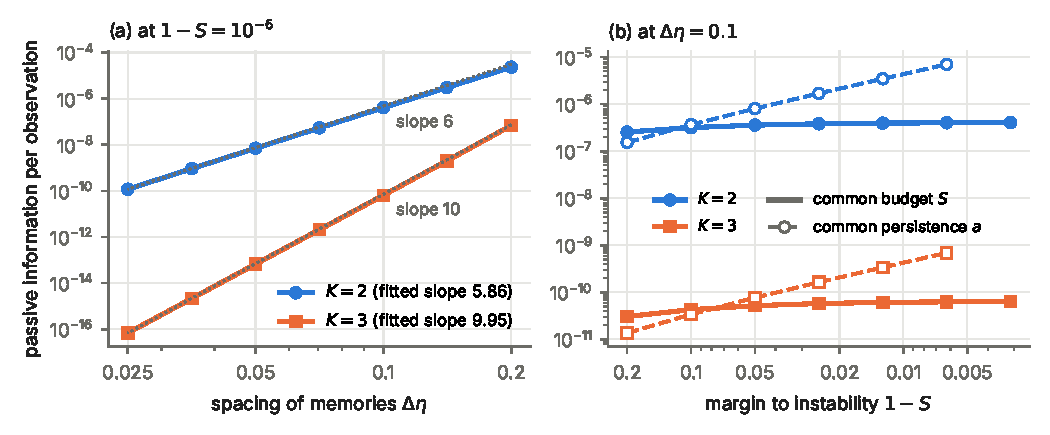
\includegraphics[width=\textwidth]{fig_barrier.pdf}
\caption{The passive barrier near instability. Both panels show the Gaussian Kullback--Leibler information per observation between the stationary price processes of two populations whose merged measures are the $K$-node Gauss and Gauss--Radau rules on memories spread over $\Delta\eta$ around $0.5$ (total weight $0.3$, impact $\kappa=0.5$). (a)~At a common feedback budget one millionth below instability, the information falls like $(\Delta\eta)^{4K-2}$ (dotted lines). (b)~Held at a common budget (solid), the information stays bounded as the margin $1-S$ shrinks; held at a common persistence (dashed), it grows without bound, because the budgets then differ. Computed from the closed-form spectra; scripts in \nolinkurl{research_extension/fragility_reveals/}.}
\label{fig:barrier}
\end{figure}


\section{Who needs composition, and what disclosure buys}\label{sec:supervision}

By Theorem~\ref{thm:eqinv}, composition is worth nothing to anyone trading on public information. It can still matter to a supervisor whose action is aimed at one group. This section gives a decision in which it does and the disclosure that removes the cost of learning it. It ends with a bound on what price-based targeting can achieve when a group can hide.

\paragraph{A decision in which attribution matters.} A supervisor must keep the feedback budget $S=a+\kappa\sum_iq_i$ below a prudential ceiling $\bar s$. It can either cut all activity uniformly or halt the largest verified class. The target is the feedback budget, not the spectral radius of the state matrix: in an already stable positive economy, imposing $S\le\bar s<1$ is a tighter prudential constraint, not a restoration of stability.


\begin{proposition}[Supervisory separation: market-wide versus targeted intervention]\label{prop:target}
Assume the positive stable model, known $a,\kappa$, and $a<\bar s<1$. Write $q_i=w_i/(1-r_i)$ and $R=S-\kappa\max_iq_i$ for the post-halt feedback budget.
\begin{enumerate}[label=(\roman*),itemsep=1pt]
\item A uniform scale $\theta$ meets the ceiling exactly when $a+\theta(S-a)\le\bar s$. Its largest feasible value is $\theta^*=\min\{1,(\bar s-a)/(S-a)\}$. The identity $S=1-\kappa/\sum_jh_j$ is algebraic; estimating this infinite sum requires a justified tail bound and an observation/noise model. It alone establishes no unconditional parametric learning rate.
\item For $K=2$, the Gauss and Gauss--Radau pair of Theorem~\ref{thm:kcohort} has limiting largest normalized weights $1/2$ and $3/4$. Thus $|S^G-S^R|=O((\Delta\eta)^3)$ and $q^R_{\max}-q^G_{\max}=W/(4(1-r_c))+O(\Delta\eta)$. For sufficiently small spacing, a nonempty interval of ceilings separates their post-halt decisions. For $N$ independent reset records with common Gaussian noise $\sigma^2 I$, both decision errors at most $1/4$ require
\[
 N\ge (2\Phi^{-1}(0.75)\sigma/\|h^G-h^R\|_2)^2
 \ge c\sigma^2(\Delta\eta)^{-6}.
\]
The record horizon and the response norm must be the same on both sides.
\item Tagged-flow estimation under Theorem~\ref{thm:discvalue}, a rate bound away from one, and a fixed nonzero decision margin gives a bounded sample requirement as the spacing shrinks. The target class must be mapped to an executable, verified class label; a largest latent atom alone supplies no such identity.
\end{enumerate}
\end{proposition}
The proof is in Supplement~\ref{app:decisionfull}. Proposition~\ref{prop:targetK} there extends part~(ii) to every $K$, with exponent $4K-2$.

\subsection{What class-tagged disclosure buys}


\begin{proposition}[Tagged flow removes the barrier]\label{prop:tagged}
Let the price $x_t$ be the causal stationary solution of the model driven by i.i.d.\ centred innovations of variance $\sigma_\xi^2\in(0,\infty)$ in a positive, stable economy, with stationary autocovariances $\gamma_x(s)=\sum_\ell c_\ell\lambda_\ell^{|s|}$ ($c_\ell\ge0$, $0\le\lambda_\ell<1$ the closed-loop modes). Suppose group $i$ has merged weight $w_i>0$ and the observer receives prices and each group's flow $\tilde u_{i,t}=u_{i,t}+\varepsilon_{i,t}$, $u_{i,t}=q_iy_{i,t}$, with i.i.d.\ centred measurement noise of finite variance $\sigma_f^2$, independent of the whole innovation sequence and hence of the whole price path. Then $\tilde u_{i,t}=r_i\tilde u_{i,t-1}+w_ix_t+e_{i,t}$ with $e_{i,t}=\varepsilon_{i,t}-r_i\varepsilon_{i,t-1}$, and the just-identified IV estimator of $\beta_i=(r_i,w_i)$ with instruments $Z_t=(x_{t-1},x_t)^\top$ satisfies $\sqrt T(\hat\beta_i-\beta_i)\to N(0,V_i)$,
\begin{equation}\label{eq:ivvar}
V_i=\Sigma_i^{-1}\Omega_i\Sigma_i^{-\top},\qquad \Sigma_i=\begin{pmatrix}w_iA_0&\gamma_x(1)\\ w_iA_1&\gamma_x(0)\end{pmatrix},\qquad \Omega_i=\sigma_f^2\bigl[(1+r_i^2)\Gamma_0-r_i(\Gamma_1+\Gamma_1^\top)\bigr],
\end{equation}
where $A_m=\sum_{s\ge0}r_i^s\gamma_x(s+m)$, $\Gamma_0=\begin{psmallmatrix}\gamma_x(0)&\gamma_x(1)\\ \gamma_x(1)&\gamma_x(0)\end{psmallmatrix}$ and $\Gamma_1=\E[Z_tZ_{t-1}^\top]$. The Jacobian determinant is
\begin{equation}\label{eq:ivdet}
\det\Sigma_i=w_i\sum_{\ell,m}c_\ell c_m\frac{1-\lambda_\ell\lambda_m}{1-r_i\lambda_m}\;>\;0 .
\end{equation}
$V_i$ depends only on group $i$'s own $(w_i,r_i)$, $\sigma_f^2$ and the price autocovariances. Two conclusions are distinct: (a) for each admissible economy, $\hat\beta_i$ has the stated limiting normal law; (b) on a uniformly stable family with stationary price variance at least $\gamma_{\min}>0$ and merged weights at least $w_{\min}>0$, the limiting covariance $V_i$ is bounded by a constant that does not depend on $|r_i-r_j|$. Statement (b) bounds the limit; it is not a central limit theorem that holds uniformly over the family.
\end{proposition}

\paragraph{Machine check.} Three pieces are machine-checked: the finite-sample reset-experiment version, with an error bound that does not depend on the spacing; the lower bound on the determinant of the population instrument matrix that does not depend on the spacing (\texttt{p1\_tagged\_iv\_determinant\_bound}); and the exact decomposition of the IV score into reporting-error terms with coefficients fixed by the price path plus two boundary terms (\texttt{p1\_iv\_boundary\_decomposition}). The stationary law of large numbers and the central limit theorem behind (a) are not machine-checked.


Each tagged flow follows $u_{i,t}=r_iu_{i,t-1}+w_ix_t$, a regression whose information about $w_i$ does not involve the other groups' rates; the closed form \eqref{eq:ivdet} matches the simulated Jacobian ($0.1330$ against $0.1322$ in a two-group economy with $4\times10^5$ periods). In simulation ($T=5{,}000$, 60 replications) the root-mean-square error of the recovered weights is flat in $\Delta\eta$ (fitted slope $0.011$, error between $5.8\times10^{-4}$ and $6.6\times10^{-4}$). This is the formal content of a disclosure regime such as a consolidated audit trail: tagging flow by participant class turns a polynomial barrier into an ordinary estimation problem.
Proposition~\ref{prop:tagged} says that tagging removes the barrier; the next result says by how much.

\begin{theorem}[Value of class-tagged disclosure]\label{thm:discvalue}
Take a rich class of Theorem~\ref{prop:esprit}: rates $r_c+\Delta\eta\,s$ with $s$ in a compact set of $\gamma$-separated ordered points that has nonempty interior and contains the Gauss and Gauss--Radau pair of Theorem~\ref{thm:kcohort}, and merged weights in a nondegenerate interval $[\omega_{\min},\omega_{\max}]$, $0<\omega_{\min}<\omega_{\max}$. In each reset experiment the observer applies a unit impulse and records the price response with independent $N(0,\sigma^2)$ noise per tap; under tagging it also records each class's flow response $f_{i,t}=w_i\sum_{s\le t}r_i^{\,t-s}h_s$ with independent $N(0,\sigma_f^2)$ noise per tap. Let $N_p$ and $N_t$ be the numbers of experiments needed, without and with tagging, for a fixed accuracy and confidence. There are constants $0<c\le C<\infty$, depending on $(\sigma,\sigma_f)$ and the class but not on $\Delta\eta$, such that
\begin{enumerate}[label=(\roman*),itemsep=1pt]
\item to recover the weights to a fixed accuracy smaller than half the weight difference between the Gauss and Gauss--Radau economies (so that recovering the weights decides between them), $c\le N_t\le C$, so $N_p/N_t\asymp(\Delta\eta)^{-(4K-2)}$;
\item to recover the rates to accuracy $c_0\Delta\eta$, for a fixed $c_0>0$ smaller than the radius of a ball contained in the class of rescaled nodes (so that no fixed guess meets the target), $c(\Delta\eta)^{-2}\le N_t\le C(\Delta\eta)^{-2}$, so $N_p/N_t\asymp(\Delta\eta)^{-(4K-4)}$.
\end{enumerate}
\end{theorem}

Proposition~\ref{prop:tagged} and Theorem~\ref{thm:discvalue} use different observation arrangements: the proposition concerns passive, stationary data with prices observed without noise, where the price is a valid instrument; the theorem concerns reset experiments with noisy prices. With noisy prices, regressing flow on the observed price is an errors-in-variables problem, which is why the theorem works from the known impulse instead.
\subsection{Partial disclosure}\label{sec:partial}

Actual regimes tag some traders and not others: Japan registers high-speed traders, India identifies algorithmic orders, and everyone else stays anonymous. Theorem~\ref{thm:discvalue} prices full tagging. The next result prices tagging some of the groups.

\begin{theorem}[Partial disclosure]\label{thm:partial}
In the reset experiments of Theorem~\ref{thm:discvalue}, let the flows of $m$ of the $K$ groups be recorded (tagged), and write $K'=K-m$ for the number of untagged groups.
\begin{enumerate}[label=(\roman*),itemsep=1pt]
\item \emph{Lower bound.} If $K'\ge2$, there are two $K$-group economies with rates in $r_c+\Delta\eta[-1,1]$ and positive weights, with identical tagged groups and with untagged groups forming the $K'$-node Gauss and Gauss--Radau pair of Theorem~\ref{thm:kcohort}, such that telling them apart from $N$ reset experiments, using the price records and the tagged flow records, with error probability below $1/4$ needs $N\ge c\,(\Delta\eta)^{-(4K'-2)}$.
\item \emph{Upper bound.} Let the tagged groups satisfy the conditions of Theorem~\ref{thm:discvalue}, and let the untagged groups range over a rich class of Theorem~\ref{prop:esprit} with $K'\ge2$ nodes. Estimate each tagged group from its flow records, subtract its contribution from the estimated kernel, and apply Prony's method with $K'$ nodes to the residual. This recovers the weights of all $K$ groups to any fixed accuracy from $N=C(\Delta\eta)^{-(4K'-2)}$ experiments.
\item \emph{One untagged group.} If $K'\le1$, the weights of all $K$ groups are recovered from a number of experiments that does not depend on $\Delta\eta$.
\end{enumerate}
The constants depend on $(\sigma,\sigma_f)$, the class and the tagged groups, not on $\Delta\eta$. So the cost of composition is that of the untagged groups alone: $N^*\asymp(\Delta\eta)^{-(4K'-2)}$ for $K'\ge2$.
\end{theorem}

\begin{proof}
(i) The two economies share the tagged groups, so their kernels differ only through the untagged pair, whose moments agree up to order $2K'-2$ (Theorem~\ref{thm:kcohort}); the kernel gap is therefore of order $(\Delta\eta)^{2K'-1}$ at every lag. The price impulse responses inherit this order through the closed-loop recursion, as in the proof of Theorem~\ref{thm:kcohort}, with constants that depend on the tagged groups only through the closed-loop stability margin. A tagged group's flow response, $f_{i,t}=w_i\sum_{s\le t}r_i^{\,t-s}h_s$, is the same linear map of the price response in both economies, so its mean difference is also of order $(\Delta\eta)^{2K'-1}$. With Gaussian noise the divergence of one experiment's full record is at most $C(\Delta\eta)^{4K'-2}$, and Le Cam's two-point lemma gives the bound.
(ii) As in the proof of Theorem~\ref{thm:discvalue}, the averaged price responses and least squares on each tagged class's flows estimate the tagged weights and rates with error $O_P(N^{-1/2})$, uniformly on the class and without dependence on $\Delta\eta$ or on the other groups. The kernel values $k_0,\ldots,k_{2K'-1}$ are smooth functions of the taps (proof of Theorem~\ref{prop:esprit}), so the residual kernel $k_j-\sum_{\rm tagged}\hat w_i\hat r_i^{\,j}$ estimates the untagged groups' kernel with error $O_P(N^{-1/2})$. Prony's method on these $2K'$ values is the estimator of Theorem~\ref{prop:esprit} with $K'$ nodes, whose error is the input error times order $(\Delta\eta)^{-(2K'-1)}$ (the rescaling of the centred moments). So the untagged weights have error $O_P(N^{-1/2}(\Delta\eta)^{-(2K'-1)})$, and $N=C(\Delta\eta)^{-(4K'-2)}$ suffices; the tagged weights are recovered at the faster rate.
(iii) With one untagged group of weight $v$ and rate $s$, $k_0=\sum_{\rm tagged}w_i+v$ and $k_1=\sum_{\rm tagged}w_ir_i+vs$, so $v$ and $s$ are smooth functions of $k_0$, $k_1$ and the tagged estimates, all estimated with error $O_P(N^{-1/2})$ independent of $\Delta\eta$. With none, this is Theorem~\ref{thm:discvalue}(i).
\end{proof}

\paragraph{The value of each tag.} Tagging one more group lowers the exponent by four while two or more groups stay untagged: the data needed fall by a factor of order $(\Delta\eta)^{-4}$. The tag that leaves a single group untagged is worth the most, a factor of order $(\Delta\eta)^{-6}$, because one untagged group needs no separating at all. The last tag is worth nothing for the weights. So a supervisor never needs to tag everyone: tagging all but one memory class gives the full composition at a cost that does not depend on how close the memories are. What matters is how many distinct memory classes remain untagged, not how many traders. A regime that tags registered high-speed traders and leaves everyone else anonymous gets the full benefit only if everyone else behaves, in memory, like a single class.

\paragraph{Numerical check and machine check.} For $K=3$ with no tag and one tag, and $K=4$ with two tags, the exact divergence per experiment of the hard pair falls with $\Delta\eta$ at fitted slopes $10.05$, $6.02$ and $5.96$, against $10$, $6$ and $6$ (\nolinkurl{research_extension/partial_disclosure/partial_disclosure_check.py}). Part~(i) is machine-checked on the joint records of prices and tagged flows, for records of any fixed length $T$ and a common noise variance $\sigma^2$ on prices and flows (with $\sigma_f\ne\sigma$, replace $\sigma$ by $\min(\sigma,\sigma_f)$): for any two economies that share their tagged groups and whose untagged node moments agree below order $n$, any test satisfies $4\sigma^2(1-\alpha_0-\beta_0)^2\le N(T+MT)\bigl(2W2^T(\Delta\eta)^nC_T(1+W_tT)\bigr)^2$ (\texttt{p1\_partial\_lower\_bound\_matched}, \nolinkurl{Paper1PartialDisclosureLower.lean}); with the matched $K'$-node pair of Theorem~\ref{thm:kcohort}, $n=2K'-1$. The algebraic steps of (ii) and (iii) are machine-checked too (\nolinkurl{Paper1PartialDisclosure.lean}); the estimation errors of (ii) and (iii) are on paper and checked by Monte Carlo: subtract-then-Prony gives weight errors growing like $(\Delta\eta)^{-(2K'-1)}$, fitted slopes $-5.07$, $-3.02$ and $0.36$ for $K'=3,2,1$ untagged groups of three, against $-5$, $-3$ and $0$ (\nolinkurl{research_extension/theorem_checks/mc_rates.py}).

\subsection{Pooling markets}\label{sec:pool}

Algorithms trade in many markets at once. A trend follower's lookback is a property of the algorithm, the same in every futures contract it trades, while how much it trades in each market varies. A supervisor who sees several markets therefore sees several kernels built from the same memory rates with different weights. The next result says what that is worth.

Take $D$ markets, each with known persistence and impact and its own independent noise, and the same $K$ algorithms with memory rates $r_i=r_c+\Delta\eta\,s_i$ in every market and merged weights $W_{ij}>0$ in market $j$. Every market is Schur stable for every configuration considered, $a_j+\kappa_j\sum_iW_{ij}/(1-r_c-\Delta\eta)<1$. In each market the supervisor runs $N$ reset experiments as in Theorem~\ref{prop:esprit}. Let $q^*=\lceil K/D\rceil$ and $l^*=K-1+q^*$.

\begin{theorem}[Pooling markets]\label{thm:pool}
\begin{enumerate}[label=(\roman*),itemsep=1pt]
\item \emph{Lower bound.} Near every configuration $(s,W)$ with distinct nodes at which the moment map below order $l^*$ has locally constant rank (an open dense set), there are two configurations at a fixed distance in $(s,W)$, with distinct nodes and positive weights, whose kernels agree in every market up to the moments of order $l^*-1$. Telling them apart with error probability below $1/4$ needs $N\ge c\,(\Delta\eta)^{-2l^*}$.
\item \emph{Upper bound.} At configurations where the rescaled moment map up to order $l^*$ has an injective differential (condition (R)), a minimum-distance estimator restricted to a neighbourhood recovers the rescaled nodes and the weights with error $O_P(N^{-1/2}(\Delta\eta)^{-l^*})$, so $N=C(\Delta\eta)^{-2l^*}$ experiments suffice locally.
\item \emph{The order is sharp.} Condition (R) never holds below order $l^*$, and it holds at generic configurations for every $K\le8$ and $D\le K$.
\item \emph{Globally.} Take a compact class of configurations with nonempty interior, separated nodes and weights bounded below. Let $l_c$ be the least order at which the moment map is injective on the class up to relabelling, and $l_g\ge l_c$ the least order at which it is, in addition, an immersion on the class. Over that class the data needed are at least of order $(\Delta\eta)^{-2l_c}$ and at most of order $(\Delta\eta)^{-2l_g}$, with $l^*\le l_c\le l_g\le2K-1$; if condition (R) holds at order $l^*$ everywhere on the class, $l_g=l_c$ and the order is exact. Pooling never needs more data than one market.
\end{enumerate}
So the data requirement is of order $(\Delta\eta)^{-2(K-1+\lceil K/D\rceil)}$: $(\Delta\eta)^{-(4K-2)}$ with one market, as in Theorem~\ref{thm:kcohort}, and $(\Delta\eta)^{-2K}$ with $K$ or more markets. Markets whose weights are linear combinations of other markets' weights add data but do not lower the exponent; $D$ is the rank of the participation matrix $W$.
\end{theorem}

\begin{proof}
Write $\mu_{jl}=\sum_iW_{ij}(r_i-r_c)^l=(\Delta\eta)^lt_{jl}$ with $t_{jl}=\sum_iW_{ij}s_i^l$; the map from $(s,W)$ to the $t_{jl}$ does not depend on $\Delta\eta$. As in the proof of Theorem~\ref{prop:esprit}, in each market the kernel values, and hence the centred moments $\mu_{jl}$, are smooth functions of the taps whose constants do not depend on $\Delta\eta$.
(i) The moments of orders $0,\ldots,l^*-1$ in all markets are $Dl^*=D(K+q^*-1)$ equations in $K(D+1)$ unknowns, and $D(q^*-1)<K$ by the definition of $q^*$, so there are fewer equations than unknowns. Where the rank is locally constant, the set of configurations with the same $t_{jl}$, $l<l^*$, is a manifold of positive dimension through $(s,W)$. Move along it by a fixed small distance $\epsilon_0$; nodes stay distinct and weights positive. The relabellings of a configuration are isolated points, so the second configuration has a different composition. Its kernels agree with the first's below order $l^*$, and from order $l^*$ on the centred moments differ by $O((\Delta\eta)^{l^*})$, with a summable bound over orders because $|r_i|<1$. The price responses inherit this order through the closed-loop recursion of each market, so the divergence of one experiment in all $D$ markets is $O((\Delta\eta)^{2l^*})$, and Le Cam's two-point lemma gives the bound. If further markets have weight vectors that are fixed linear combinations of these $D$ markets' weights, the same combinations along the curve keep their moments below order $l^*$ equal as well, and their weights stay positive for a small move; so such markets do not change the exponent.
(ii) The estimated taps give $\hat\mu_{jl}$ with error $O_P(N^{-1/2})$, hence $\hat t_{jl}=(\Delta\eta)^{-l}\hat\mu_{jl}$ with error $O_P(N^{-1/2}(\Delta\eta)^{-l^*})$ for $l\le l^*$. Under (R) the map $(s,W)\mapsto(t_{jl})_{l\le l^*}$ is an immersion; on a neighbourhood its image is a manifold on which the map has a Lipschitz inverse, and the minimum-distance estimator, which projects $\hat t$ onto that image, inherits the error.
(iv) \emph{Lower bound.} If $l_c>l^*$, by the definition of $l_c$ the class contains two configurations that are not relabellings of each other and share all moments below order $l_c$; their distance is positive and does not depend on $\Delta\eta$, and the two-point argument of part~(i) gives $N\ge c(\Delta\eta)^{-2l_c}$. If $l_c=l^*$, part~(i) applied at an interior point of constant rank gives the same order. And $l_c\ge l^*$, because by part~(i) the moment map below order $l^*$ is not injective near such a point. \emph{Upper bound.} An injective immersion of a compact set is an embedding with a Lipschitz inverse on its image, so the minimum-distance estimator over the class has error $O_P(N^{-1/2}(\Delta\eta)^{-l_g})$. If (R) holds at order $l^*$ on the whole class, it holds at every higher order, since rows are only added, so the map is an immersion at order $l_c$ and $l_g=l_c$. And $l_g\le2K-1$ because one market's moments up to order $2K-1$ determine its $K$ nodes and weights (Prony), with injective differential, after which every other market's weights solve a nonsingular Vandermonde system.
(iii) Below order $l^*$ there are fewer equations than unknowns, so the differential cannot be injective. Generic validity of (R) is a polynomial condition: it holds outside a proper algebraic set as soon as it holds at one configuration, and an exact computation (rank modulo a large prime at random integer configurations, which certifies full rank over the rationals) confirms it for every $K\le8$, $D\le K$.
\end{proof}

\paragraph{What this means.} An algorithm's memory is the same everywhere it trades, and that is what gives it away. Pooling price records from markets where the same algorithms trade in different proportions lowers the exponent of the composition barrier, from $4K-2$ to $2(K-1+\lceil K/D\rceil)$, without any disclosure. Cross-market surveillance is a partial substitute for tagging. The converse is a constraint on hiding: to stay as hidden as in a single market, the algorithms must trade in the same proportions in every market, so that the participation matrix has rank one. For two algorithms with half-lives between 5 and 9 days (memory rates $0.9\pm0.025$, total weight $0.06$, impact $0.5$, feedback budget $0.9$, passive Gaussian records), the Gauss and Gauss--Radau pair needs about $7{,}000$ years of daily prices in one market. In two markets in which the algorithms' shares differ by $50$ percentage points, the hardest pair found by a numerical search needs about $90$ years; with shares differing by $20$ points, about $4{,}000$. At half the memory spacing the one-market figure rises to $400{,}000$ years and the two-market figures to about $1{,}300$ and $55{,}000$. The gain grows like $(\Delta\eta)^{-2}$ as memories approach each other, and it depends on how differently the algorithms allocate across markets. These two-market figures come from a numerical search for the hardest pair under stated constraints; the true worst case can only be harder.

\paragraph{Relation to the literature, and checks.} The mathematics is the multi-snapshot version of super-resolution, where several observations of the same nodes with different amplitudes are known to improve resolution \citep{li2022}; the closed-form exponent for $D$ deterministic snapshots and its use in markets are, to our knowledge, new. The exponent is confirmed by the smallest singular value of the Jacobian in 60-digit arithmetic (local slopes $3,2$; $5,4,3$; $7,5,5,4$ for $K=2,3,4$) and by exact rank computations (\nolinkurl{research_extension/cross_market/}, which also holds the calibration scripts). The counting steps are machine-checked (\texttt{p1\_pool\_rows\_lt}, \texttt{p1\_pool\_rows\_ge}, \texttt{p1\_pool\_single\_market}, \texttt{p1\_pool\_many\_markets} in \nolinkurl{Paper1PoolingMarkets.lean}). Whether $l_c=l^*$ is a global question that the theorem leaves open. Numerical searches for other positive configurations sharing all moments up to order $l^*$, with 400 starts at each of 15 random configurations per case, find none for $(K,D)=(2,2),(3,2),(3,3),(4,2),(4,4)$ at configurations whose nodes are separated. Every apparent solution found lies within $0.05$ of a configuration that has two nearly coincident nodes (gap below $0.04$), with residuals just under the search tolerance; these are directions in which the moment map is ill-conditioned, not distinct configurations of a class with separated nodes. This is consistent with $l_c=l^*$ in all five cases but does not prove it. When $D$ divides $K$ the system at order $l^*$ is square, and several solutions could occur in other regions (\nolinkurl{research_extension/cross_market/global_fibres.py}, \nolinkurl{global_fibres_extended.py}, \nolinkurl{global_fibres_inspect.py}). Monte Carlo runs of the local estimator of part~(ii), with the search started at the true configuration, confirm the attained rates: the weight error grows like $(\Delta\eta)^{-l^*}$ with fitted slopes $-3.02$, $-1.98$, $-4.92$ and $-2.95$ for $(K,D)=(2,1),(2,2),(3,1),(3,3)$, against $-3,-2,-5,-3$ (\nolinkurl{research_extension/theorem_checks/mc_rates.py}). The lower bound on joint records of all markets is machine-checked for any matched pair (\texttt{p1\_pool\_lower\_bound\_matched}, \nolinkurl{Paper1PoolingLower.lean}), with an explicit pair for two algorithms in two markets (\texttt{p1\_pool\_explicit\_pair\_K2D2}). Not covered: markets with cross-impact, and algorithms whose memory differs across markets.

\subsection{Traders who respond to being watched}\label{sec:hiding}

The results so far take the groups' rules as given. A group that expects a targeted action has a reason to change its rule. Sufficiency bounds what a supervisor who relies on prices can then achieve.

\begin{proposition}[Hiding caps targeting]\label{prop:hiding}
A supervisor observes prices, under any probes and for a record of any length, and then targets a given group or not. Being targeted costs the group $P>0$. The group chooses among available rules. Rule $\rho$ has a private cost $C(\rho)\ge0$ and leads to targeting with probability $\pi(\rho)$. Suppose one available rule $\rho_0$, with cost $C_0$, gives the population the kernel of a population that the supervisor targets with probability $\alpha$.
\begin{enumerate}[label=(\roman*),itemsep=1pt]
\item $\pi(\rho_0)=\alpha$, whatever the supervisor's probes, record length and decision rule.
\item Every rule $\rho^*$ that minimizes the group's expected cost $C(\rho)+P\pi(\rho)$ satisfies
\[
\pi(\rho^*)\ \le\ \alpha+\frac{C_0-C(\rho^*)}{P}\ \le\ \alpha+\frac{C_0}{P}.
\]
\item Suppose the group has two rules: its original rule, with cost zero and targeting probability $\pi_T$ on a record of length $T$, and $\rho_0$. It adopts $\rho_0$ whenever $\pi_T>\alpha+C_0/P$. If $\pi_T\to1$ and $P(1-\alpha)>C_0$, this holds for all large $T$, and the targeting probability is then $\alpha$.
\end{enumerate}
\end{proposition}

\begin{proof}
(i) By Theorem~\ref{thm:eqinv}, populations with the same kernel give the same law of the price record for every probe sequence and every insider and dealer rule. The supervisor's decision is a function of that record and of its own randomization. (ii) $C(\rho^*)+P\pi(\rho^*)\le C_0+P\alpha$ by optimality, and $C(\rho^*)\ge0$. (iii) The original rule costs $P\pi_T$ and $\rho_0$ costs $C_0+P\alpha$.
\end{proof}


\section{Beyond the kernel: saturating traders and stress}\label{sec:saturating}

The kernel is a linear object, and every precedent for it is linear. Real feedback traders have limits: position caps, margin, risk budgets. This section asks what replaces the kernel when trades saturate, and what prices reveal about the part that saturation adds. The answer is a sharper version of the paper's main message. In calm markets, prices reveal the kernel and nothing else. How close traders are to their limits, which is what governs behaviour under stress, is invisible in calm data. It can be learned only by pushing traders toward their limits, or from disclosure.

\paragraph{Saturating traders.} In the market of Theorem~\ref{thm:eqinv}, let trader $i$ have memory rate $r_i\in[0,1)$, capacity $c_i>0$ and leverage $\ell_i\in\mathbb R$. Its memory state is $m_{i,t}=\sum_{j<t}r_i^{\,t-1-j}s_j$, as before, and its flow is
\[
 f_{i,t}=c_i\,\psi(\ell_i m_{i,t}),
\]
for a policy shape $\psi$ common to all traders. A shape is \emph{band-linear} if $\psi(u)=u$ for $|u|\le1$. The hard limit $\psi(u)=\max(-1,\min(1,u))$ is the leading case: inside its band trader $i$ trades $c_i\ell_im_{i,t}$, and at the band edge its position is capped at $c_i$. Inside the bands the population is the linear one of Section~\ref{sec:model}, with merged weights $w_i=c_i\ell_i$ and kernel $k_m=\sum_ic_i\ell_ir_i^m$. Write
\[
 \nu=\sum_ic_i\,\delta_{(r_i,\ell_i)}
\]
for the capacity-weighted measure on memory and leverage.

\begin{theorem}[What replaces the kernel]\label{thm:satsuff}
For any shape $\psi$, aggregate feedback flow is $f_t=\sum_ic_i\psi(\ell_im_{i,t})=\int\psi\bigl(\ell\,m_t(r)\bigr)\,\nu(dr,d\ell)$, with $m_t(r)=\sum_{j<t}r^{t-1-j}s_j$, so it depends on the population only through $\nu$. If two populations have the same $\nu$, that is $\sum_ic_ig(r_i,\ell_i)=\sum_jc'_jg(r'_j,\ell'_j)$ for every function $g$, then for every strategy profile and every realization the price and order-flow paths, the insider's trades and profit and the dealer's inventory coincide at every date. The two games have the same equilibria under any equilibrium concept defined from payoffs and the public history. The kernel is the first leverage moment of $\nu$ at each memory, $k_m=\int r^m\ell\,d\nu$, and in general it does not determine $\nu$.
\end{theorem}


The proofs of Theorems~\ref{thm:satsuff}--\ref{thm:stress} and Proposition~\ref{prop:smooth} are in Supplement~\ref{app:saturating}.

\paragraph{Machine check.} \nolinkurl{Paper1SaturatingSufficiency.lean} proves the pathwise statement for every shape $\psi$ and every causal insider, dealer and signal rule (\texttt{p1\_sat\_sufficiency}, through the generic \texttt{p1\_flow\_market\_invariance}). The passage to equilibria is on paper, as in Theorem~\ref{thm:eqinv}.

\begin{theorem}[No information without stress]\label{thm:stress}
Let $\psi$ and $\psi'$ be band-linear. Take two populations $P$ and $P'$ with the same kernel, $\sum_ic_i\ell_ir_i^m=\sum_jc'_j\ell'_jr_j'^{\,m}$ for every $m$, but possibly different capacities and leverages.
\begin{enumerate}[label=(\roman*),itemsep=1pt]
\item \emph{Pathwise.} Run both markets with the same strategy profile and the same realization. Let $\tau$ be the first date at which some trader of $P$ or of $P'$, with its state computed from the signals of the $P$-market, leaves its band ($|\ell m_t|>1$). Then the two markets have identical price and order-flow paths on every date $t<\tau$. On those dates both also coincide with the \emph{linear} market with kernel $k$, so $\tau$ is the first exceedance date of the linear market.
\item \emph{Records.} Let $O_T$ be any record that is a function of the paths on dates $t<T$, plus noise independent of them. The laws of $O_T$ under $P$ and $P'$ satisfy
\[
 \mathrm{TV}\bigl(\mathcal L_P(O_T),\mathcal L_{P'}(O_T)\bigr)\le\Pr\nolimits_{\rm lin}(\tau<T),
\]
the probability that some trader of $P\cup P'$ leaves its band before $T$ in the linear market.
\item \emph{Calm passive data.} In the market of Section~\ref{sec:model} with innovations $\varepsilon_t\sim N(0,\sigma_\varepsilon^2)$ i.i.d., no probe, a start from rest, and a linear market with $S_{\rm abs}=a+\kappa\sum_m|k_m|<1$, let $s_r^2=\sup_t\mathrm{Var}_{\rm lin}(m_t(r))$ and $\vartheta=\max_g|\ell_g|s_{r_g}$ over the $n+n'$ traders of $P\cup P'$. Then
\[
 \mathrm{TV}\le T\,(n+n')\,e^{-1/(2\vartheta^2)},\qquad s_r\le\frac{\sigma_\varepsilon}{(1-r)(1-S_{\rm abs})},
\]
and any test that tells $P$ from $P'$ with both error probabilities at most $\alpha<1/2$ needs $T\ge(1-2\alpha)\,e^{1/(2\vartheta^2)}/(n+n')$ observations.
\item \emph{Probes.} Without process noise, if the linear market's response to a deterministic probe keeps every trader of $P\cup P'$ inside its band, the two records have the same law, for any number of repetitions and any observation noise. For a single pulse of size $A$, no information is obtained below
\[
 A^*=\min_g\Bigl(|\ell_g|\,\sup_t\Bigl|\sum_{j<t}r_g^{\,t-1-j}h_j\Bigr|\Bigr)^{-1},
\]
with $h$ the linear impulse response.
\end{enumerate}
\end{theorem}


\paragraph{Machine check.} The pathwise part (i), including the statement that the market follows the linear market until the first exceedance, is machine-checked for every pair of band-linear shapes and every causal insider, dealer and signal rule (\texttt{p1\_sat\_stress\_invariance}, \texttt{p1\_sat\_follows\_linear}, \texttt{p1\_satAggFlow\_linear\_of\_band}). Parts (ii)--(iv) are on paper.

\paragraph{An example, and what differs at stress.} At memory $r=0.7$, take $P=\{(c,\ell)=(1,0.1)\}$ and $P'=\{(0.25,0.2),(1,0.05)\}$. Both have merged weight $0.1$, so they have the same kernel and are equivalent until stress. Under a hard limit, their total capacities, the largest aggregate flow they can deliver, are $1$ and $1.25$ (\texttt{p1\_sat\_capacity\_differs}). In the market of Section~\ref{sec:model} with $a=0.5$ and $\kappa=0.8$, single pulses up to size $4$ give exactly identical responses. Larger pulses push the most levered trader of $P'$ to its limit, and the responses separate by $0.072$ at size $6$ and $0.364$ at size $12$. Under Gaussian innovations, the simulated probability that some trader leaves its band within $1{,}000$ dates lies below the bound of part (iii) at every noise level tested. It is zero up to $\sigma_\varepsilon=0.3$, and $0.0175$, $0.0875$ and $0.63$ at $\sigma_\varepsilon=0.35$, $0.4$ and $0.5$. The scripts are \nolinkurl{research_extension/nonlinear_scoping/sim_wiener.py} and \nolinkurl{sim_passive_clip.py}. Figure~\ref{fig:twolayer} shows the two layers.

\begin{figure}[t]\centering
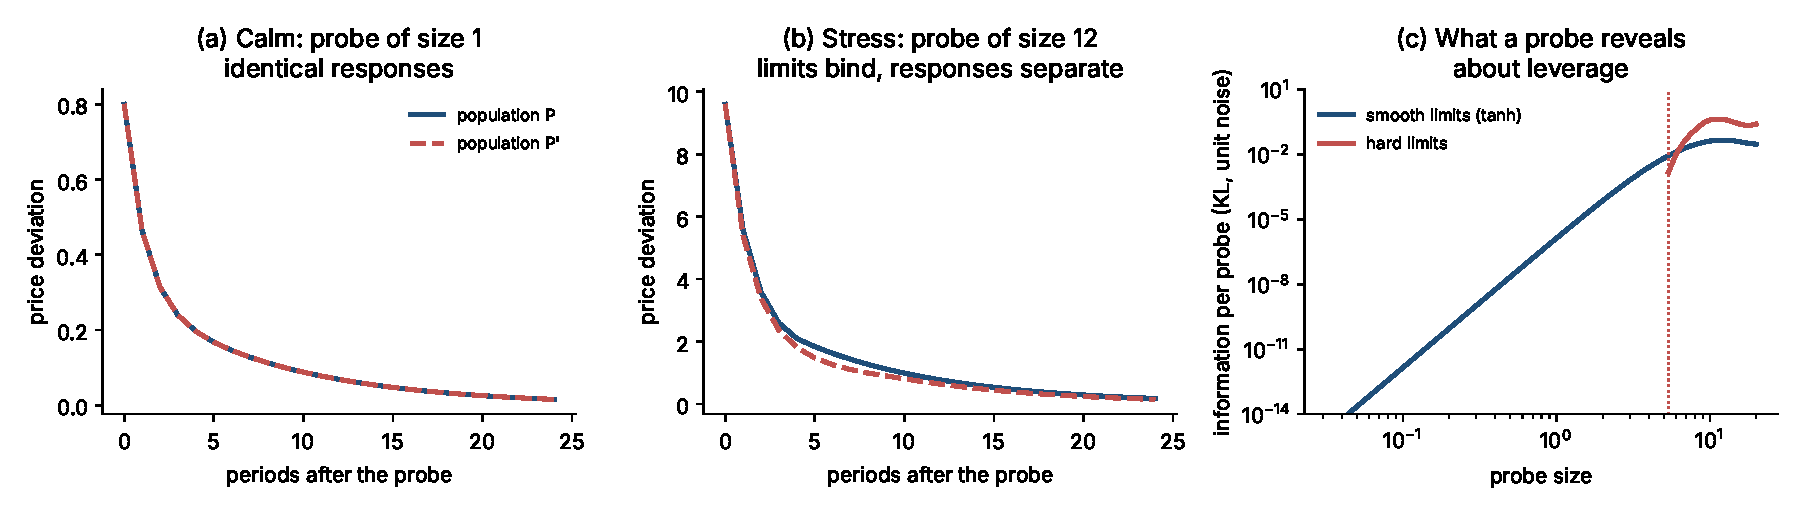
\includegraphics[width=\textwidth]{figs_core/fig_twolayer.pdf}
\caption{The two layers. Populations $P=\{(c,\ell)=(1,0.1)\}$ and $P'=\{(0.25,0.2),(1,0.05)\}$ at memory $0.7$ have the same kernel ($a=0.5$, $\kappa=0.8$). (a)~Under hard limits, a calm probe gives identical responses. (b)~A stress probe pushes the most levered trader to its limit and the responses separate. (c)~Information per probe about the difference (Kullback--Leibler divergence over 30 taps, unit noise): under smooth limits it grows like the sixth power of the probe size (fitted slope $6.00$); under hard limits it is exactly zero below the size at which the first trader reaches its limit ($5.38$, dotted).}\label{fig:twolayer}
\end{figure}

\begin{proposition}[Smooth saturation: information grows like the sixth power of the probe]\label{prop:smooth}
Let $\psi=\tanh$. In the probing experiment of Section~\ref{sec:model}, with reset state, no process noise, a single pulse of size $A$ and taps observed with independent $N(0,\sigma^2)$ noise, compare two populations $P$ and $P'$ with the same kernel and with $\rho_P=a+\kappa\sum_ic_i|\ell_i|/(1-r_i)<1$, and likewise $\rho_{P'}<1$. Let $\hat S=\max(\rho_P,\rho_{P'})$, $\Lambda_P=\tfrac13\sum_ic_i|\ell_i|^3/(1-r_i)^3$, and $\Delta M_3=\sum_ic_i\ell_i^3-\sum_jc'_j\ell_j'^{\,3}$.
\begin{enumerate}[label=(\roman*),itemsep=1pt]
\item The two price responses satisfy $\|x^P-x^{P'}\|_2\le C_D|A|^3$ with $C_D=\kappa^4(\Lambda_P+\Lambda_{P'})/(1-\hat S)^2$. Hence $N$ experiments that tell $P$ from $P'$ with both errors at most $\alpha<1/2$ need
\[
 N\ge\frac{4\sigma^2(1-2\alpha)^2}{C_D^2\,A^6}.
\]
\item The first tap after the pulse differs by $x_1^P-x_1^{P'}=-\tfrac13\kappa^4\Delta M_3A^3+O(A^5)$. If $\Delta M_3\ne0$, then for all small enough $|A|$ the averaged first tap tells $P$ from $P'$ with error at most $\alpha$ once $N\ge\bigl(12\,\sigma\,\Phi^{-1}(1-\alpha)\bigr)^2/(\kappa^8\Delta M_3^2A^6)$. So the order $A^{-6}$ is attained. The cubic coefficient of the first tap identifies $\sum_ic_i\ell_i^3$, the third leverage moment of $\nu$.
\end{enumerate}
\end{proposition}



\subsection{What stress reveals}

Theorem~\ref{thm:stress} says what calm data cannot show. The next result says what stress does show: everything that matters. Write
\[
 \tilde\mu=\sum_ic_i\,\mathrm{sgn}(\ell_i)\,\delta_{(r_i,|\ell_i|)}
\]
for the signed capacity at each memory and each leverage level. A trend follower and a contrarian with the same memory and the same leverage magnitude offset exactly, since $c\,\psi(-\ell m)=-c\,\psi(\ell m)$ for odd $\psi$.

The result holds for any shape with one property. An odd shape $\psi$ has \emph{independent dilations} if rescaled copies of it at distinct scales are linearly independent: for any distinct $s_1,\ldots,s_n>0$ and any weights $w_1,\ldots,w_n$, $\sum_kw_k\psi(s_ku)=0$ for every $u$ implies $w_1=\cdots=w_n=0$.

\begin{theorem}[Stress identifies the leverage distribution]\label{thm:satident}
Let $\psi$ be odd with independent dilations, and let every trader have $r_i\ge0$ and $\ell_i\ne0$. In the probing experiment of Section~\ref{sec:model}, with reset state and exactly observed responses, two populations give identical price responses to every probe sequence if and only if $\tilde\mu_P=\tilde\mu_{P'}$. Probe responses therefore identify, within each memory class, the net capacity at every leverage level. The kernel $k_m=\int\lambda r^m\,\tilde\mu(dr,d\lambda)$ is one linear functional of this measure.

The property holds or fails as follows.
\begin{enumerate}[label=(\roman*),itemsep=1pt]
\item The hard limit has independent dilations. For it the result needs probes of all sizes: probes that keep every memory state inside every band identify only the kernel (Theorem~\ref{thm:stress}(iv)).
\item $\tanh$ has independent dilations. Moreover, identical responses to all probes in an arbitrarily small neighbourhood of zero already imply $\tilde\mu_P=\tilde\mu_{P'}$.
\item A cubic shape $\psi(u)=u-\gamma u^3$ does not: the scales $1,2,3$ with weights $5,-4,1$ give $\sum_kw_k\psi(s_ku)=0$ for every $u$. For such a shape, probes identify only the first and third leverage moments within each memory.
\end{enumerate}
\end{theorem}

\paragraph{Machine check.} The general statement of Theorem~\ref{thm:satident} is machine-checked for any number of traders (\texttt{p1\_thm\_stress\_identification} in \nolinkurl{Paper1StressIdentificationGeneral.lean}). So are the first sentence of part~(i) (\texttt{p1\_clip\_indep\_dilations}), the first sentence of part~(ii) (\texttt{p1\_tanh\_indep\_dilations}) and the counterexample in part~(iii) (\texttt{p1\_cubic\_not\_indep\_dilations}). The theorem for the two shapes, with no hypothesis left on $\psi$, is \nolinkurl{p1_thm_stress_identification_hard_limit} and \nolinkurl{p1_thm_stress_identification_tanh}. Two things are proved on paper only: the small-probe statement in part~(ii), and the last sentence of part~(iii). In the formal statement, ``identical responses'' reads: every pair of a probe and a price path of the first market is such a pair of the second.

The proof (Supplement~\ref{app:saturating}) uses three facts. First, probes can steer the price along any path, so identical responses mean identical maps from past prices to flow. Second, two dates of prices turn that map into a sum of scaled copies of $\psi$, one per memory--leverage pair, with distinct scales for a suitable direction. Third, independent dilations separate the copies. For the hard limit, each copy adds a kink where its pair saturates, and the copy with the largest scale has the first kink. For $\tanh$, each copy approaches its limit at its own exponential rate, and the copy with the smallest scale has the slowest tail. The kink argument is constructive. In the example of Figure~\ref{fig:twolayer}, read along one direction, the flow map has kinks at $3.702$ and $14.813$, and their slope jumps return net capacities $0.24989$ and $0.99988$, against true values $0.25$ and $1$. Locating the second group needs a memory state of almost $15$, about four times the stress level at which the first trader saturates. Knowing the kernel and the first group fixes only the second group's total $c\ell$, not its leverage.

The theorem assumes exactly observed responses; with observation noise, a minimum-distance estimator recovers $\tilde\mu$ consistently, without a rate (Supplement Proposition~\ref{prop:noisystress}). Theorem~\ref{thm:satident} turns Section~\ref{sec:saturating} into a two-layer theory. Prices in calm markets identify the kernel. Prices under stress identify the full signed measure $\tilde\mu$, which by Theorem~\ref{thm:satsuff} is all that any price-based outcome depends on. Under hard limits, no information beyond the kernel arrives until the first group saturates. Under smooth limits, the order-$n$ term of the response scales with the probe size to the power $2n+1$. We expect its information to scale with the power $2(2n+1)$, but only the case $n=1$ is proved (Proposition~\ref{prop:smooth}).

\subsection{Deleveraging traders and dealers who anticipate}

\begin{proposition}[Deleveraging traders]\label{prop:delever}
Let each trader follow any causal rule, for example deleveraging gradually, liquidating, or switching strategy after a loss, provided it trades linearly, $w_im_{i,t}$, as long as its state has stayed inside its band on every date up to $t$. Then Theorem~\ref{thm:stress} holds verbatim for two such populations with the same kernel. Up to the first date at which some trader leaves its band, the paths coincide and equal the linear market's path, and parts (ii)--(iv) follow.
\end{proposition}

The proof of the pathwise part is the induction of Theorem~\ref{thm:stress}(i). It is machine-checked for arbitrary causal rules outside the bands (\texttt{p1\_delever\_stress\_invariance}). Deleveraging that starts before a hard limit only moves the band edge inward. Calm data remain silent until the first trader starts to cut its position.

\paragraph{After the first breach: an open question.} What happens after a breach is not covered by these results. A natural conjecture is a threshold. If traders who breach their limits liquidate, their sales move the price, and the price move pushes other traders' states toward their own limits. One expects a cascade when the liquidation triggered per unit of price move, summed over the traders close to their limits, exceeds the market's capacity to absorb it, and no cascade otherwise. We have no proof of such a threshold and do not state one.

\begin{proposition}[Who sets prices matters]\label{prop:dealers}
\begin{enumerate}[label=(\roman*),itemsep=1pt]
\item Theorems~\ref{thm:stress} and~\ref{thm:satident} and Proposition~\ref{prop:delever} hold for any causal dealer rule that is the same in the two markets. This covers every rule that depends on the population only through its kernel, for example a dealer who knows only the kernel, or one who prices current flow.
\item A dealer who knows the population and quotes on the expected next-period feedback flow uses more than the kernel. Suppose the next memory states are Gaussian, $m^+_g\sim N(\bar m_g,s_g^2)$, with every trader inside its band in expectation, $|\ell_g\bar m_g|<1$, and hard limits. Then the expected next-period flows under two populations with the same kernel differ by at most
\[
 \sum_{g\in P\cup P'}c_g\sqrt{2/\pi}\;\sigma_g\,e^{-\delta_g^2/(2\sigma_g^2)},\qquad \sigma_g=|\ell_g|s_g,\quad\delta_g=1-|\ell_g\bar m_g|.
\]
\end{enumerate}
\end{proposition}

The proof is in Supplement~\ref{app:saturating}.

\paragraph{What the supervisor can and cannot learn.} The two results split the population into a part prices reveal in calm markets, the kernel, and a part they reveal only under stress: the distribution of leverage within each memory, weighted by capacity. The second part decides how the market behaves when traders hit their limits, through the total capacity and through how many traders are near their limits. Calm-market price data are therefore the wrong instrument for it, however long the record and however sophisticated the estimator. The options are stress probes, whose cost and risk Proposition~\ref{prop:smooth} prices, actual stress episodes, or disclosure of capacities: position limits, margins and risk budgets. This is a different disclosure from the class-tagged flow of Section~\ref{sec:supervision}. Tagged flow reveals each group's memory and weight. Capacity disclosure reveals how far each group is from its limit.

\subsection{Any population}\label{sec:anypop}

The results above describe two families of rules: linear rules, summarized by the kernel, and saturating rules, summarized by the measure $\nu$. The next theorem drops the family. A population is now represented only by its aggregate feedback flow map $F$, which sends a price path to the flow at each date and may be any causal function: linear, saturating, deleveraging, or switching between strategies after observing past profits.

\begin{theorem}[Any population]\label{thm:anypop}
In the probing experiment of Section~\ref{sec:model}, with reset state, exactly observed responses and $\kappa\ne0$, let two populations have aggregate flow maps $F$ and $F'$.
\begin{enumerate}[label=(\roman*),itemsep=1pt]
\item \emph{Sufficiency.} If $F=F'$ on every price path, the two markets give the same prices, order flows, insider profits and dealer inventories for every strategy profile and realization, and the same equilibria.
\item \emph{Identification.} If every pair of a probe sequence and a price path produced by the first population is produced by the second, then $F=F'$ on every price path. So the two populations give identical responses to every probe sequence if and only if $F=F'$, and a group-level quantity, such as the weight of the largest group, is identified from probe responses if and only if it is a function of $F$.
\item \emph{Cost.} Let $\mathcal C$ be any class of populations that contains the two linear $K$-group economies of Theorem~\ref{thm:kcohort}(i). Then any procedure that decides a group-level quantity separating them, over $\mathcal C$, from $N$ reset impulse-response records needs $N\ge c\,\sigma^2(\Delta\eta)^{-(4K-2)}$, and from passive Gaussian records needs at least the number of observations of Theorem~\ref{prop:passive}. For impulse-response records, every band-linear class whose capacities can be large enough that the impulse responses keep every trader inside its band contains populations with exactly the two economies' responses; for passive Gaussian records, the same holds up to an arbitrarily small loss in the error probabilities if the capacities in the class are unbounded.
\end{enumerate}
\end{theorem}

\begin{proof}
Part~(i) is the induction of Theorem~\ref{thm:eqinv}, which uses only that the flow is a fixed causal function of past public signals. For part~(ii), given any price path $x^*$, the probe $v_t=(x^*_t-ax^*_{t-1})/\kappa-F(x^*)_t$ makes the first market follow $x^*$, because the flow at date $t$ depends only on prices before $t$. By hypothesis the second market also follows $x^*$ under this probe, and subtracting the two price equations gives $F(x^*)_t=F'(x^*)_t$ at every date. The converse is part~(i) applied to the probing recursion. A quantity $g$ is identified exactly when $g$ agrees on populations with identical responses, that is, on populations with the same $F$. For part~(iii), a procedure that works over $\mathcal C$ works in particular on the two economies, so the lower bounds of Theorems~\ref{thm:kcohort} and~\ref{prop:passive} apply. For a band-linear class, take capacities $c_i$ and leverages $\ell_i=w_i/c_i$ with $c_i$ large enough that $|\ell_im_{i,t}|\le1$ along the impulse response, which is bounded; inside the bands each trader trades $c_i\ell_im_{i,t}=w_im_{i,t}$, so the population reproduces the linear economy's responses (Theorem~\ref{thm:stress}(i)). Under passive Gaussian innovations the bands are eventually left, so exact equality fails; but for a record of $T$ dates, Theorem~\ref{thm:stress}(iii) bounds the total-variation distance between the band-linear and the linear laws by $T\,K\,e^{-1/(2\vartheta^2)}$, and $\vartheta\to0$ as the capacities grow with the merged weights fixed. A procedure with errors $\alpha,\beta$ on the band-linear pair therefore has errors at most $\alpha+\delta,\beta+\delta$ on the linear pair, for any $\delta>0$, and the passive bound applies with $1-\alpha-\beta-2\delta$ in place of $1-\alpha-\beta$.
\end{proof}

\paragraph{What this changes, and what it does not.} Part~(ii) is the general form of Theorems~\ref{thm:merged} and~\ref{thm:satident}: prices identify the aggregate flow map and nothing finer, for any population. For linear rules the map is the kernel, which determines the merged measure; for odd saturating shapes with independent dilations it determines the signed capacity measure; for a cubic shape it determines only two leverage moments. Which group-level quantities prices reveal is therefore a property of the family of rules, and it can be read off from how the family maps to flow maps. Part~(iii) says that allowing richer rules cannot make composition cheaper to learn than in the linear case, because the hard linear pair remains in the class. What is not proved is an upper bound for general classes: for some families composition is not identified at all (the cubic shape), and for others the attainable rate is open.

\paragraph{Machine check.} Parts (i) and (ii) are machine-checked for an arbitrary flow map: \texttt{p1\_flow\_market\_invariance} (\nolinkurl{Paper1SaturatingSufficiency.lean}); \texttt{p1\_general\_identification}, \texttt{p1\_general\_identification\_iff}, \texttt{p1\_responses\_of\_flow\_eq} and \texttt{p1\_identified\_functional} (\nolinkurl{Paper1GeneralIdentification.lean}). The band-linear embedding in part~(iii) uses \texttt{p1\_sat\_follows\_linear}. The transfer of the lower bounds is on paper. Numerically, for a population that switches between a trend-following and a contrarian strategy according to past profits, the steering probe of the proof drives the market to a random target path to machine precision and recovers the flow map to $2\times10^{-16}$, while a population with a different switching intensity departs from the path (\nolinkurl{research_extension/theorem_checks/mc_stress_and_general.py}).

\paragraph{What is open.} Three questions remain open. The first is rates for the higher orders of Theorem~\ref{thm:satident}: Proposition~\ref{prop:smooth} gives the first nonlinear moment, and the general order is not proved. The second is a full equilibrium with forward-looking dealers and saturating or deleveraging traders, including what happens after the first breach, in a fire sale. The third is learning agents whose rules change continuously, not only at a band edge. Related ideas appear in the literature on funding constraints and liquidity spirals \citep{brunnermeier2009} and in evidence that crowding predicts tail risk \citep{barroso2022}. The identification of sums of nonlinear branches is a known problem in system identification \citep{dreesen2017}. What is new here is the sufficient measure inside a strategic market, the exact absence of calm-market information about it, and the reduction of its recovery under stress to a known uniqueness problem.

\section{Scope and limits}\label{sec:scope}

\paragraph{Linearity.} Sufficiency (Theorem~\ref{thm:eqinv}, Proposition~\ref{prop:anylinear}) needs aggregate feedback flow to be a linear function of past public signals, plus independent idiosyncratic shocks if there are any. With group-specific Gaussian demand shocks, a second aggregate enters, the spectral density of the aggregate shock process, and the equivalence class shrinks accordingly (Supplement~\ref{app:eqinv}). The passive results of Section~\ref{sec:cost} are stated for Gaussian innovations. With non-Gaussian innovations, higher-order moments of prices could carry further information; we do not analyse that case. Saturating rules are treated in Section~\ref{sec:saturating}. Other nonlinear rules, and traders who change their rules as they learn, are outside the theorems. \citet{niroula2026a} report simulations of stylized nonlinear rules and of online learners trained in the closed loop. In those simulations, the costs of Section~\ref{sec:cost} hold when the competing populations' feedback weights match. Populations whose learned weights differ are told apart by those weights instead. Hard thresholds hide groups from small probes altogether. These are simulations, not theorems.

\paragraph{Exponential memory.} The identification and cost results need memory to be a finite mixture of exponentials. For general completely monotone memory, \citet{niroula2026a} prove that the minimax accuracy for the memory distribution is of exact order $1/\log(N/\sigma^2)$. Halving the error then squares the data needed, instead of multiplying it by a constant.

\paragraph{The observer.} The lower bounds hold for an observer who knows $(a,\kappa)$ and the noise law, so they hold a fortiori without that knowledge. The upper bounds assume reset experiments or a known initial state. Strategic responses to being observed are modelled only in Proposition~\ref{prop:hiding}, and there for one group. Everywhere else the groups do not change their rules when probed.

\paragraph{Evidence.} \citet{niroula2026a} report pre-specified tests on two sets of trader-class reports: the CFTC's weekly Commitments of Traders in twenty futures markets and Binance's class ratios in 30 perpetual markets. Of 23 recorded outcomes, 11 pass. None is a direct test of a result in this paper: all use class positions or account ratios rather than executed flow tagged by class. The class reports constrain the persistence of class positions far more tightly than prices do. They do not identify learning memory, because that persistence can also reflect turnover, reporting aggregation or inventory retention. A pre-registered out-of-sample test of the feedback premise on Taiwan's tagged exchange flows (spec P1T, holdout 2019--2023; \citet{niroula2026a} report every diagnostic) gives the following. $D=0.0426$ $[0.0206, 0.0643]$, $p=0.000$, meets the registered supportive criterion. The pre-specified reverse-causality check gives $D=-0.0065$ $[-0.0316, 0.0165]$, which does not meet it. The registered verdict is `supportive'. Read with its pre-specified diagnostic, the test does not provide evidence of feedback beyond prices revealing past flow. We do not claim that tagged flow in Taiwan responds to price deviations. The registered test is supportive, but its pre-specified diagnostic attributes the gain to reverse causality.

A second test, of the two-layer prediction of Section~\ref{sec:saturating}, is registered on Binance perpetual futures (spec P7S, amendment A1). Its primary sample is retrospective (July 2024 to October 2026), specified in November 2026 after the sample period, and a prospective window from November 2026 serves as a replication. The primary test was run once on 11 November 2026. A pre-specified test on Binance perpetual futures was inconclusive (calm difference $-0.002$, 90\% interval $[-0.007, 0.004]$; difference-in-differences $0.041$, $p=0.553$). It neither supports nor contradicts the prediction of Section~\ref{sec:saturating}. The prospective replication covers 16 November 2026 to 14 February 2027; its symbols and thresholds were fixed on its own development data (August to October 2026) before the window opened, and its result is not yet available.

\paragraph{Open problems.} Four questions remain open: a long-lived strategic insider who times her trades against the groups' memory; rates for the higher orders of the identification of saturating traders, and a full equilibrium with forward-looking dealers and deleveraging traders after a breach; sufficiency for learning agents whose rules change; and a supervisory loss function estimated from real interventions, which would turn the information costs here into a value of disclosure.



\section{Proofs of the main results}\label{app:proofs}

\paragraph{A lemma used in the proofs.}
\begin{lemma}[Positive price-response geometry]\label{lem:cm}
In the positive, stable economy the impulse response is a nonnegative mixture of decaying exponentials,
\[
h_j=\sum_\ell \omega_\ell\lambda_\ell^j,\qquad \omega_\ell\ge0,\quad \sum_\ell\omega_\ell=\kappa,\quad 0\le\lambda_\ell<1 .
\]
It is completely monotone and nonincreasing; its peak is the direct impact $\kappa$, even though $J$ is non-normal. In price/memory coordinates the price-only gain is $\sup_t\|e_x^\top J^t\|_2=1$.
\end{lemma}

\paragraph{Lemma~\ref{lem:cm}.} Omit zero-weight groups. For $a>0$ put $b_i=\kappa q_i$ and
\[
T={\rm diag}\bigl(\sqrt a,\sqrt{b_1/\eta_1},\ldots\bigr),\qquad u=\bigl(\sqrt a,\sqrt{b_1\eta_1},\ldots\bigr)^\top .
\]
The price-first transition becomes the symmetric matrix $J'=TJT^{-1}={\rm diag}(0,r_1,\ldots)+uu^\top$, the input transforms to $\kappa u$ and $J'e_x=\sqrt a\,u$, so $h_j=(\kappa/a)e_x^\top(J')^{j+1}e_x$. The spectral decomposition of $J'$ gives nonnegative weights summing to $h_0=\kappa$, and Schur stability puts the eigenvalues in $[0,1)$. The case $a=0$ follows by continuity. A nonnegative mixture of decaying geometric sequences is completely monotone. Since $J$ is nonnegative with row sums at most one, every price row of $J^t$ has $\ell_1$, hence $\ell_2$, norm at most one, attained at $t=0$.


\paragraph{Lemma~\ref{lem:micro}.} (i) For $v_{t+1}=v_t+\zeta_{t+1}$ and $r_t=v_t+\nu_t$, the steady-state prior variance $P$ solves $P=P\sigma_\nu^2/(P+\sigma_\nu^2)+\sigma_\zeta^2$, i.e.\ $P^2-\sigma_\zeta^2P-\sigma_\zeta^2\sigma_\nu^2=0$, whose positive root is $P=\bigl(\sigma_\zeta^2+\sqrt{\sigma_\zeta^4+4\sigma_\zeta^2\sigma_\nu^2}\bigr)/2$. The gain is $\eta=P/(P+\sigma_\nu^2)\in(0,1)$, which simplifies to \eqref{eq:kgain}, and the update $\hat v_{t+1}=\hat v_t+\eta(r_t-\hat v_t)$ has the stated form. (ii) $\nabla_\theta\tfrac12H(x_t-\theta)^2=-H(x_t-\theta)$, so $\theta_{t+1}=(1-\gamma)\theta_t+\alpha H(x_t-\theta_t)=(1-\eta)\theta_t+\eta qx_t$ with $\eta=\gamma+\alpha H$ and $q=\alpha H/\eta$.


\paragraph{Theorem~\ref{thm:merged}.} With zero initial states, $y_{i,t}=\sum_{s\le t}\eta_ir_i^{t-s}x_s$, so $\sum_iq_iy_{i,t}=\sum_{s\le t}k_{t-s}x_s$ and every response is determined by $(a,\kappa,k)$, hence by $M$. Conversely, equal responses for all probes imply equal $H$, hence equal $G$, and partial fractions of $G$ identify the distinct poles with nonzero residues $w_i$, i.e.\ $M$. After cancellation, $H=\kappa zD(z)/[(z-a)D(z)-\kappa N(z)]$ with $D=\prod(z-r_i)$ and $N(z)=\sum_iw_iz\prod_{j\ne i}(z-r_j)$, as in \eqref{eq:H}; at a retained $r_i$ the denominator equals $-\kappa N(r_i)=-\kappa w_ir_i\prod_{j\ne i}(r_i-r_j)\neq0$ (memory rates are positive because $\eta_i<1$), so no root of $D$ cancels. The numerator $\kappa zD(z)$ has no roots other than $0$ and the $r_i$, so these are the only possible cancellations. The remaining numerator factor $z$ cancels if and only if the denominator vanishes at $0$; since $N(0)=0$ the denominator there equals $-aD(0)$, which is nonzero for $a>0$ and zero for $a=0$. Hence the McMillan degree, which is the dimension of a minimal realization, is $1+|{\rm supp}(M)\cap(0,1)|$ for $a'\neq0$ and $|{\rm supp}(M)\cap(0,1)|$ for $a'=0$ (an atom at rate $0$, a group with $\eta=1$, contributes the constant $M(\{0\})$ to $G$ and no pole, so it shifts $a$ to $a'=a+\kappa M(\{0\})$ and the argument above applies with $a'$) (numerically, the rank of the Hankel matrix of $(h_j)_{j\ge1}$ is $K+1$ and $K$ respectively for $K=1,2,3$). For (ii), direct algebra gives
\[
G_\delta(z)-G_0(z)=-\frac{qz(z-1)\delta^2}{(z-1+\bar\eta)\bigl((z-1+\bar\eta)^2-\delta^2\bigr)} .
\]
The denominator is the product of the three linear factors $z-r$ with $r\in\{1-\bar\eta,\,1-\bar\eta\pm\delta\}$, all in $[\epsilon,1-\epsilon]$ by assumption; on $|z|=1$ each satisfies $|z-r|\ge1-r\ge\epsilon$, so $|G_\delta-G_0|\le2q\delta^2/\epsilon^3$ there. Uniform stability gives $M_H=\sup|H_\theta|<\infty$, and the identity $H_\delta-H_0=z^{-1}H_\delta H_0(G_\delta-G_0)$, whose factor $z^{-1}$ has modulus one on the circle, gives an $\ell_2$ gain at most $C_{\mathcal F}\delta^2$. The mean difference of a power-constrained probe has squared norm at most $C_{\mathcal F}^2\delta^4PT$; the equal-noise KL is at most $C_{\mathcal F}^2\delta^4PT/(2\sigma_\nu^2)$, and Pinsker's inequality with total variation at least $1-2\alpha$ gives \eqref{eq:Tpower}.


\paragraph{Theorem~\ref{thm:kcohort}.} Let $(s^A,\omega^A)$ and $(s^B,\omega^B)$ be the $K$-point Gauss and Gauss--Radau rules for the uniform weight on $[-1,1]$, normalized to unit mass. Both are positive and exact for polynomials of degree $2K-2$, and their moments of degree $2K-1$ differ by $g_K\neq0$. To see that $g_K\ne0$, let the Radau nodes be $-1,s_2,\ldots,s_K$ and put $P(s)=(s+1)\prod_{j\ge2}(s-s_j)^2$. This is monic of degree $2K-1$ and vanishes at every Radau node, so the Radau rule gives it $0$. Gauss is exact to degree $2K-1$, so it gives $\int P\,d\mu>0$, since $P\ge0$ on $[-1,1]$ and vanishes only at the nodes. The two rules agree on every lower-degree term, so they differ on $s^{2K-1}$. Put $r=r_c+\Delta\eta\,s$ and weights $W\omega$, and let $\mu^X_j=W\sum_i\omega^X_i(s^X_i)^j$ for $X\in\{A,B\}$. Then $|\mu^X_j|\le W$, and $\mu^A_j=\mu^B_j$ for $j\le2K-2$.

\emph{Kernel gap.} By the binomial theorem, $k^X_m=\sum_j\binom mj r_c^{m-j}(\Delta\eta)^j\mu^X_j$. So, with $n=2K-1$, $\Delta k_m=k^A_m-k^B_m=\sum_{j\ge n}\binom mj r_c^{m-j}(\Delta\eta)^j(\mu^A_j-\mu^B_j)$. Since $\binom mj\le\binom mn\binom{m-n}{j-n}$ for $j\ge n$, this gives $|\Delta k_m|\le2W\binom mn(\Delta\eta)^n(r_c+\Delta\eta)^{m-n}$. Summing with $\sum_m\binom mn x^{m-n}=(1-x)^{-(n+1)}$ gives $\|\Delta k\|_1\le2W(\Delta\eta)^{2K-1}/(1-r_c-\Delta\eta)^{2K}$ over all lags.

\emph{Response gap.} Let $\varsigma=a+\kappa W/(1-r_c-\Delta\eta)<1$, the theorem's hypothesis. Each kernel has $\|k^X\|_1\le W/(1-r_c-\Delta\eta)$. From $h_0=\kappa$ and $h_{t+1}=ah_t+\kappa\sum_jk_jh_{t-j}$, every partial sum of $|h^B|$ is at most $\kappa/(1-\varsigma)$. The difference $\Delta h=h^A-h^B$ has $\Delta h_0=0$ and $\Delta h_{t+1}=a\Delta h_t+\kappa\sum_j\bigl(k^A_j\Delta h_{t-j}+\Delta k_jh^B_{t-j}\bigr)$, so every partial sum of $|\Delta h|$ is at most $\kappa\|\Delta k\|_1\|h^B\|_1/(1-\varsigma)$. Hence, for every horizon,
\[
\|h^A-h^B\|_2\le\|h^A-h^B\|_1\le C_U(\Delta\eta)^{2K-1},\qquad C_U=\frac{2\kappa^2W}{(1-r_c-\Delta\eta)^{2K}(1-\varsigma)^2}.
\]
In the other direction, $\Delta k_j=0$ for $j<2K-1$, so by induction $\Delta h_t=0$ for $t\le2K-1$, and $\Delta h_{2K}=\kappa\,\Delta k_{2K-1}h^B_0=\kappa^2Wg_K(\Delta\eta)^{2K-1}$. When the taps $h_0,\ldots,h_{T-1}$ are observed with $T\ge2K+1$, this gives $\|h^A-h^B\|_2\ge\kappa^2W|g_K|(\Delta\eta)^{2K-1}$. With $T\le2K$ the observed responses coincide. The impossibility bound holds for every $T$, since it uses only the upper order.

\emph{Testing.} $N$ reset experiments have divergence $N\|h^A-h^B\|_2^2/(2\sigma^2)$. By Pinsker's inequality, a test whose two error probabilities are at most $\alpha$ needs divergence at least $2(1-2\alpha)^2$. So $N\ge4(1-2\alpha)^2\sigma^2(\Delta\eta)^{-(4K-2)}/C_U^2$, and the constant does not depend on $T$. For the $W_1$ version, the two merged measures are the images of the fixed normalized rules under $s\mapsto r_c+\Delta\eta\,s$ scaled to mass $W$, so their distance is $W\Delta\eta$ times the distance $2c_K>0$ between the rules, and the same two-point argument applies with the metric loss.


\paragraph{Theorem~\ref{prop:passive}.} For stationary Gaussian processes with spectral densities $f_j\propto|H_j(e^{i\omega})|^2$, the divergence rate is
\[
D=\frac1{4\pi}\int_{-\pi}^{\pi}\bigl(\varrho-1-\log\varrho\bigr)\,d\omega,\qquad \varrho=f_1/f_0=|H_1/H_0|^2 .
\] By the resolvent identity, $H_1/H_0-1=z^{-1}H_1\Delta G$ with $\Delta G=G_1-G_0$, and uniform stability bounds $|H_1|$ on the circle, so $u\equiv\varrho-1=2\,{\rm Re}(z^{-1}H_1\Delta G)+O(|\Delta G|^2)$. Write $G(z)=\sum_kw_k\phi(z,\eta_k)$, with $w_k$ the group weights (any factor of $\eta_k$ is absorbed in $\phi$), where $\phi$ is analytic in $\eta$ on a neighbourhood of $[\eta_{\min},\eta_{\max}]$ uniformly for $|z|=1$ (its pole $z=1-\eta$ stays inside the disk). Expanding $\phi$ around $\bar\eta$, $\Delta G=\sum_{j\ge0}\frac{\partial_\eta^j\phi(z,\bar\eta)}{j!}\,\Delta\tilde M_j$, where $\tilde M_j=\sum_kw_k(\eta_k-\bar\eta)^j$. For the pair, $\Delta\tilde M_0=\Delta\tilde M_1=0$ and $\Delta\tilde M_2=q\delta^2$; for the moment-matched economies, $\Delta\tilde M_j=0$ for $j\le2$ and $\Delta\tilde M_3=4\tau p_-p_+(\Delta\eta)^3$ by \eqref{eq:dM3}; for the $K$-group Gauss and Gauss--Radau economies with rates $\bar\eta+\Delta\eta\,s$ and weights $W\omega$, both rules integrate polynomials of degree $2K-2$ exactly, so $\Delta\tilde M_j=W(\Delta\eta)^j\sum_k(\omega^A_k(s^A_k)^j-\omega^B_k(s^B_k)^j)$ vanishes for $j\le2K-2$ and equals $\pm Wg_K(\Delta\eta)^{2K-1}\neq0$ at $j=2K-1$. Higher terms are smaller by a factor of the spacing: $|\Delta\tilde M_j|\le2W(\Delta\eta)^j$, and analyticity of $\phi$ in $\eta$ on a disk of radius $\varrho>0$ around $\bar\eta$, uniformly on the circle, gives $|\partial_\eta^j\phi|/j!\le C\varrho^{-j}$, so for $\Delta\eta<\varrho/2$ the tail beyond the first nonzero term is $O((\Delta\eta)^{j_0+1})$. Hence $\sup_\omega|u|=O(\delta^2)$, $O(\tau(\Delta\eta)^3)$, respectively $O((\Delta\eta)^{2K-1})$, and $u=c(\omega)\epsilon+o(\epsilon)$ with $\epsilon=\delta^2$, $\tau(\Delta\eta)^3$ or $(\Delta\eta)^{2K-1}$ and $c(\omega)$ proportional to $2\,{\rm Re}\bigl(z^{-1}H_0\,\partial^{j_0}_\eta\phi(\cdot,\bar\eta)\bigr)/j_0!$, $j_0=2$, $3$ or $2K-1$. The function $c$ does not vanish identically: $f=z^{-1}H_0\partial^j_\eta\phi$ is analytic outside the disk including at infinity, where it vanishes, and is not identically zero; an analytic function on the exterior whose real part vanishes on the circle is an imaginary constant, which here would have to be zero. For $|u|\le\frac12$, $u^2/4\le u-\log(1+u)\le u^2$, so $D\asymp\int c(\omega)^2d\omega\,\epsilon^2$, which gives (i)--(iii). The sample requirements need a finite-$T$ bound that is uniform in the separation, which we obtain directly. The first $T$ observations are $N(0,\Sigma_j)$ with $\Sigma_j$ the $T\times T$ Toeplitz matrices of the spectral densities $f_j=\sigma^2|H_j(e^{i\omega})|^2$. On the compact, uniformly stable family the transfer functions have no zeros or poles on the circle (Theorem~\ref{thm:minphase}), so $0<\underline f\le f_j\le\bar f<\infty$ with constants that do not depend on the separation. A Toeplitz matrix has eigenvalues within the range of its symbol, so $\lambda_{\min}(\Sigma_0)\ge\underline f$ and $\|\Sigma_1-\Sigma_0\|\le\sup_\omega|f_1-f_0|=\sup_\omega f_0|u|\le\bar f\sup_\omega|u|$. With $A=\Sigma_0^{-1/2}\Sigma_1\Sigma_0^{-1/2}$, whose eigenvalues lie in $[\underline f/\bar f,\bar f/\underline f]$, the inequality $\lambda-1-\log\lambda\le(\lambda-1)^2/\lambda$ gives
\[
\KL(P_1^T\|P_0^T)=\tfrac12\sum_k(\lambda_k-1-\log\lambda_k)\le\frac{\bar f}{2\underline f}\,\|A-I\|_F^2\le\frac{\bar f}{2\underline f}\,T\Bigl(\frac{\bar f}{\underline f}\Bigr)^2\sup_\omega|u|^2\le C\,T\epsilon^2,
\]
with $C$ independent of $T$ and of the separation, because $\sup_\omega|u|=O(\epsilon)$ uniformly. The Bretagnolle--Huber inequality \citep[Lemma 2.6]{tsybakov2009} then gives the stated lower bounds on $T$ for every $T$, not only asymptotically. For a fixed pair, $T^{-1}\KL(P_1^T\|P_0^T)\to D$ and Stein's lemma (one error fixed) and the Chernoff bound (both errors vanishing) give the error exponents of the likelihood-ratio test, of the same order in the separation; that statement is pointwise in the pair.


\paragraph{Theorem~\ref{thm:minphase}.} In the delay variable $\lambda=z^{-1}$, $H=\kappa\prod_i(1-r_i\lambda)/\bigl[(1-a\lambda)\prod_i(1-r_i\lambda)-\kappa\lambda\sum_iw_i\prod_{j\ne i}(1-r_j\lambda)\bigr]$, which is \eqref{eq:H} divided through by $z^{K+1}$; its nonstructural zeros are the memory rates, which do not cancel under the nondegenerate assumptions of Theorem~\ref{thm:minphase}. In the z-plane there is also the structural timing zero at zero: the numerator is proportional to $z\prod_i(z-r_i)$. Stability puts the poles inside the disk. A rational spectral density $\sigma^2|H(e^{i\omega})|^2$ has a unique minimum-phase factor up to a unimodular constant, which is $H$; Theorem~\ref{thm:merged} then gives the merged measure.


\paragraph{Proposition~\ref{prop:tagged}.} With tagged flow, $u_{i,t}=r_iu_{i,t-1}+w_ix_t$ holds exactly and involves only group $i$, so $\tilde u_{i,t}=r_i\tilde u_{i,t-1}+w_ix_t+e_{i,t}$ with the MA(1) error $e_{i,t}$. Prices are independent of the measurement noise, so $\E[Z_te_{i,t}]=0$ and, by the ergodic theorem for the stationary linear price process, the IV estimator is consistent when $\Sigma_i=\E[Z_t(\tilde u_{i,t-1},x_t)]$ is nonsingular. Since $u_{i,t-1}=w_i\sum_{s\ge0}r_i^sx_{t-1-s}$, $\E[x_{t-1}u_{i,t-1}]=w_iA_0$ and $\E[x_tu_{i,t-1}]=w_iA_1$, which gives $\Sigma_i$. The price is a nonnegative mixture of geometric responses to its innovation (Lemma~\ref{lem:cm}), so $\gamma_x(s)=\sum_\ell c_\ell\lambda_\ell^{s}$ with $c_\ell=\sigma_\xi^2\kappa^{-2}\omega_\ell\sum_m\omega_m/(1-\lambda_\ell\lambda_m)\ge0$; substituting, $\det\Sigma_i=w_i(\gamma_x(0)A_0-\gamma_x(1)A_1)=w_i\sum_{\ell,m}c_\ell c_m(1-\lambda_\ell\lambda_m)/(1-r_i\lambda_m)$, each term positive. By summation by parts, $\sum_{t=1}^TZ_te_{i,t}=\sum_{t=1}^T(Z_t-r_iZ_{t+1})\varepsilon_{i,t}+O_P(1)$. Since $(\varepsilon_{i,t})$ is i.i.d.\ with mean zero and variance $\sigma_f^2$ and independent of the whole stationary price process, the summands $m_t=(Z_t-r_iZ_{t+1})\varepsilon_{i,t}$ form a stationary ergodic martingale difference sequence with respect to $\mathcal F_t=\sigma((x_s)_{s\in\mathbb Z},\varepsilon_{i,s}:s\le t)$, with $\E[m_tm_t^\top]=\sigma_f^2[(1+r_i^2)\Gamma_0-r_i(\Gamma_1+\Gamma_1^\top)]=\Omega_i$, so the Billingsley--Ibragimov martingale central limit theorem gives \eqref{eq:ivvar}. On a uniformly stable family the modes and weights lie in a compact set with $\lambda_\ell\le\bar\lambda<1$, so with $w_i\ge w_{\min}>0$ we get $\det\Sigma_i\ge w_{\min}(1-\bar\lambda^2)\gamma_x(0)^2>0$ and $\|\Omega_i\|$ is bounded, uniformly in the spacing.


\paragraph{Theorem~\ref{prop:esprit}.}
\begin{proof}
The kernel values $k_m=\sum_iw_ir_i^m$ are the power moments of the merged measure. The closed-loop recursion $h_t=ah_{t-1}+\kappa\sum_mk_mh_{t-1-m}$ (plus $\kappa$ at $t=0$) can be solved for $k_0,\ldots,k_{2K-1}$ from $h_1,\ldots,h_{2K}$. Because $h_0=\kappa$ is a known primitive, each $k_m$ is a polynomial in $h_1,\ldots,h_{m+1}$ with coefficients depending on $(a,\kappa)$ (the only division is by $\kappa h_0=\kappa^2$), so on the bounded set of responses within sup-distance $1$ of the class this map is $L_h$-Lipschitz, with $L_h$ depending on the class but not on $\Delta\eta$. Let $E$ be the event $\max_{1\le t\le2K}|\bar h_t-h_t|\le\sigma N^{-1/2}\sqrt{2\log(4K/\beta)}$, where $\bar h_t$ averages the $N$ responses; a Gaussian tail bound and a union bound over the $2K$ estimated taps give $P(E)\ge1-\beta$. On $E$, and provided this radius is at most $1$, the estimated kernel values satisfy $\max_m|\hat k_m-k_m|\le L_h\sigma N^{-1/2}\sqrt{2\log(4K/\beta)}$. Centring at $r_c$ is a fixed triangular linear map, $\mu_m=\sum_{j\le m}\binom mj(-r_c)^{m-j}k_j$, and $\mu_m=(\Delta\eta)^m t_m$ with $t_m=\sum_iw_is_i^m$. The map $F:(s,\omega)\mapsto(t_0,\ldots,t_{2K-1})$ does not depend on $\Delta\eta$; its Jacobian is a confluent Vandermonde matrix with determinant $\prod_i\omega_i\prod_{i<j}(s_i-s_j)^4$, bounded away from zero on the compact class. On ordered, $\gamma$-separated nodes $F$ is injective, because a measure with $K$ distinct atoms is determined by its first $2K$ moments. A $C^1$ map that is injective on a compact set $Q$ and has a nonsingular Jacobian there is injective on an open neighbourhood $U$ of $Q$: otherwise there are $x_n\ne y_n$ with $F(x_n)=F(y_n)$ and distance to $Q$ tending to zero, whose limits $x,y\in Q$ satisfy $F(x)=F(y)$, so $x=y$, contradicting local injectivity at $x$. Applying the quantitative inverse function theorem uniformly on $Q$, there are $\rho_0>0$ and $L<\infty$, uniform over the class, such that $F(U)$ contains the ball of radius $\rho_0$ around every point of $F(Q)$ and the single inverse $F^{-1}:F(U)\to U$ is $L$-Lipschitz on each such ball. An error $e$ in $\mu_m$ is an error $e(\Delta\eta)^{-m}$ in $t_m$, largest at $m=2K-1$. Since $\Delta\eta<1$ and the centring map is fixed, on $E$ we get $\|\hat t-t\|_\infty\le C_1\sqrt{\log(4K/\beta)}\,\epsilon_N$ with $C_1$ equal to $\sqrt2L_h$ times the norm of the centring map; and because $\sigma N^{-1/2}\sqrt{2\log(4K/\beta)}\le\sqrt2\,\epsilon_N\sqrt{\log(4K/\beta)}$, the radius condition holds whenever $c_0\le1/\sqrt2$. When this is below $\rho_0$, $\hat t$ lies in the ball where $F^{-1}$ is $L$-Lipschitz. For an input in such a ball, $x=F^{-1}(\hat t)$ has $K$ distinct nodes and nonzero weights, so the $K\times K$ Hankel matrix of $\hat t$ is nonsingular and Prony's method returns exactly $x$: the Prony polynomial is determined uniquely by the Hankel system, and since the $K$ real nodes of $x$ reproduce $\hat t$ it equals $\prod_i(z-\hat s_i)$, so its roots are real and distinct and no complex pair can appear; Prony's method computes the algebraic inverse of the moment map up to the order of the atoms, so, listing its output in increasing order of rate (which the error bound below keeps unambiguous once $C\sqrt{\log(4K/\beta)}\,\epsilon_N<\gamma/2$), its output is $F^{-1}(\hat t)$ and the stated bound follows with $C=LC_1$ and $c_0=\min\{\min(\rho_0,\gamma/(2L))/C_1,\,1/\sqrt2\}$, which also keeps $C\sqrt{\log(4K/\beta)}\,\epsilon_N<\gamma/2$. No separate root-perturbation bound is needed: on the ball where $F^{-1}$ is $L$-Lipschitz, Prony's roots and weights are the coordinates of $F^{-1}(\hat t)$, so the conditioning of the root step is part of $L$ (for an explicit step-by-step analysis of Prony's method with clustered exponents see \citealp{katz2023}). The matching statement requires the class to contain the Gauss and Gauss--Radau pair of Theorem~\ref{thm:kcohort} (ordered nodes with separation at least the smaller of their two minimum gaps, and weights within $[\omega_{\min},\omega_{\max}]$ after scaling to total weight $W$); for any such class the orders match, with constants that depend on the class.
\end{proof}
\paragraph{Theorem~\ref{thm:discvalue}.}
\begin{proof}
$N_p\asymp\sigma^2(\Delta\eta)^{-(4K-2)}$ by Theorems~\ref{thm:kcohort} and~\ref{prop:esprit}. \emph{Upper bounds.} Average the $N$ price responses to estimate $h$ with error of order $\sigma N^{-1/2}$ per tap. Given $h$, class $i$'s mean flow is a two-parameter family $F(w_i,r_i;h)$ whose Jacobian columns $\sum_sr_i^{t-s}h_s$ and $w_i\sum_s(t-s)r_i^{t-s-1}h_s$ are linearly independent, with a Gram determinant bounded below uniformly on the class because $w_i\ge\omega_{\min}$, the rates lie in a compact subset of $(0,1)$ and $h_0=\kappa>0$; the bound does not involve the other classes or $\Delta\eta$. Least squares on class $i$'s flows with the plug-in $h$ therefore estimates $(w_i,r_i)$ with error $O_P(N^{-1/2})$, uniformly on the class, which gives the upper bounds in (i) and in (ii) for accuracy $\epsilon\Delta\eta$. For (i) there is also a finite-sample version: in the first period the tagged flow of class $i$ is $w_i\kappa$, so the mean of the $N$ first-period records gives $P(|\hat w_i-w_i|\ge\epsilon)\le\sigma_f^2/(N\kappa^2\epsilon^2)$ by Chebyshev's inequality, for every configuration (this step is machine-checked). \emph{Lower bounds.} At a configuration in the interior of the class, perturb one class's weight by $\epsilon$, or its rate by $\epsilon\Delta\eta$; for small $\epsilon$ both perturbed configurations remain in the class because the weight interval is nondegenerate and the rate set has nonempty interior. The mean differences of both the price and the flow records are of order $\epsilon$, respectively $\epsilon\Delta\eta$, so the Kullback--Leibler divergence of $N$ experiments is at most $CN\epsilon^2$, respectively $CN\epsilon^2(\Delta\eta)^2$, and Le Cam's two-point lemma gives the lower bounds.
\end{proof}

\paragraph{Unknown primitives.}
\begin{corollary}[Unknown primitives cost nothing in the rate]
\label{cor:unknown_primitives}
In the setting of Theorem~\ref{prop:esprit}, suppose in addition that every memory rate is at least $\varepsilon>0$ (that is, $r_c-\Delta\eta\ge\varepsilon$), and that the fundamental value $p^*$, the impact $\kappa\in[\underline\kappa,\overline\kappa]\subset(0,\infty)$ and the persistence $a\in[0,\bar a]\subset[0,1)$ are unknown. Put $\tilde k_0=k_0+a/\kappa$ and $\tilde k_m=k_m$ for $m\ge1$.
\begin{enumerate}[label=(\roman*)]
\item The response depends on $(a,\kappa,M)$ only through $\kappa$ and $\tilde k$: $h_0=\kappa$ and $h_{t+1}=\kappa\sum_{m=0}^{t}\tilde k_mh_{t-m}$. The persistence $a$ acts exactly like an extra group with memory rate zero and merged weight $a/\kappa$.
\item The taps $h_0,\ldots,h_{2K+1}$ identify $(\kappa,a,M)$: $\kappa=h_0$; the recursion gives $\tilde k_0,\ldots,\tilde k_{2K}$; the values $\tilde k_1,\ldots,\tilde k_{2K}$ are the moments of orders $0,\ldots,2K-1$ of $\mu'=\sum_iw_ir_i\,\delta_{r_i}$; and $a=\kappa(\tilde k_0-\sum_iw_i)$.
\item Subtract the pre-probe price to remove $p^*$ (doubling the noise variance), estimate $\hat\kappa=\hat h_0$, deconvolve with $\hat\kappa$ alone, apply Prony's method to the estimated moments of $\mu'$, and set $\hat w_i=\widehat{w_ir_i}/\hat r_i$ and $\hat a=\hat\kappa(\hat{\tilde k}_0-\sum_i\hat w_i)$. There are constants $c_0,C>0$ depending on $(K,\mathcal S,\gamma,\omega_{\min},\omega_{\max},\varepsilon,\underline\kappa,\overline\kappa,\bar a,r_c)$ but not on $\Delta\eta$ such that, whenever $\epsilon_N\le c_0$,
\[
\max_i|\hat w_i-w_i|+|\hat a-a|+|\hat\kappa-\kappa|\;\le\;C\sqrt{\log(8K/\beta)}\;\epsilon_N
\]
with probability at least $1-\beta$. Hence $N=C'\sigma^2(\Delta\eta)^{-(4K-2)}$ experiments suffice, the same order as with known primitives.
\end{enumerate}
\end{corollary}

\begin{proof}[Proof of Corollary~\ref{cor:unknown_primitives}]
(i) Substitute $k_0=\tilde k_0-a/\kappa$ in $h_{t+1}=ah_t+\kappa\sum_{m\le t}k_mh_{t-m}$: the term $ah_t$ cancels against $\kappa(a/\kappa)h_t$. (ii) Solving the recursion of (i) for $\tilde k_t$ gives $\tilde k_t=(h_{t+1}-\kappa\sum_{m<t}\tilde k_mh_{t-m})/\kappa^2$, a polynomial in $h_1,\ldots,h_{t+1}$ divided by a power of $h_0=\kappa$. For $m\ge1$, $\tilde k_m=\sum_iw_ir_i^m=\sum_i(w_ir_i)r_i^{m-1}$, so $\tilde k_1,\ldots,\tilde k_{2K}$ are the moments of orders $0,\ldots,2K-1$ of $\mu'$, which has $K$ distinct atoms with positive weights; these moments determine $\mu'$ (Theorem~\ref{thm:merged}). Since $r_i\ge\varepsilon>0$, $w_i=(w_ir_i)/r_i$, and then $a=\kappa(\tilde k_0-\sum_iw_i)$. (iii) On the event that every estimated tap is within $\sigma N^{-1/2}\sqrt{2\log(8K/\beta)}$ of its mean (probability at least $1-\beta/2$ by the Gaussian tail and a union bound over $2K+2$ taps, with the doubled variance absorbed into the constant), $\hat\kappa\ge\underline\kappa/2$ once $\epsilon_N\le c_0$, so the map from taps to $\hat{\tilde k}$ is Lipschitz with a constant that depends on $(K,\underline\kappa,\overline\kappa,\bar a,W)$ and not on $\Delta\eta$. The weights of $\mu'$ lie in $[\varepsilon\omega_{\min},\omega_{\max}]$ and its rates are those of the class of Theorem~\ref{prop:esprit}; the proof of that theorem uses only a $\Delta\eta$-free Lipschitz deconvolution, the rescaling by $(\Delta\eta)^{-m}$ and weights bounded below, so it applies verbatim to $\mu'$ and gives $\max_i|\widehat{w_ir_i}-w_ir_i|\le C_1\sqrt{\log(8K/\beta)}\,\epsilon_N$ and rate errors smaller by a factor $\Delta\eta$, with probability at least $1-\beta/2$. The maps $(v,r)\mapsto v/r$ on $r\ge\varepsilon/2$ and $(\kappa,\tilde k_0,w)\mapsto\kappa(\tilde k_0-\sum_iw_i)$ are Lipschitz on the bounded set reached, and $|\hat\kappa-\kappa|$ and $|\hat{\tilde k}_0-\tilde k_0|$ are of order $\sigma N^{-1/2}\le\epsilon_N$. Combining gives the bound.
\end{proof}
\paragraph{Proposition~\ref{prop:anylinear}.} The proof is given after the statement in the main text.

\section{Equilibrium: further results and proofs}\label{app:eqinv}

\begin{corollary}[Disclosure in equilibrium]\label{cor:eqdisclosure}
Take a positive-impact equilibrium of Theorem~\ref{thm:inventory} with positive weights and $D>\max_ir_i$.
\begin{enumerate}[label=(\roman*),itemsep=1pt]
\item The groups' flows obey $u_{i,t+1}=r_iu_{i,t}+w_ix_t$ with their \emph{true} weights. The price is the stable closed loop of Theorem~\ref{thm:eqreduced}, driven by $\xi$, with positive effective weights. So Proposition~\ref{prop:tagged} applies: tagged flow identifies each group's $(r_i,w_i)$, with a limiting covariance that has no singularity as rates collide.
\item On classes in which both the true and the effective weights lie in compact positive intervals, Theorem~\ref{thm:discvalue} holds in equilibrium. Tagging cuts the experiments needed by a factor of order $(\Delta\eta)^{-(4K-2)}$ for weights and $(\Delta\eta)^{-(4K-4)}$ for rates.
\end{enumerate}
\end{corollary}

\paragraph{In words.} What makes disclosure valuable survives the dealers' optimization. Prices still hide the groups at the same polynomial cost, and each group's own flow still reveals that group's memory and weight directly.
\begin{theorem}[Fragility: where liquidity disappears]\label{thm:fragility}
Let there be one feedback group with weight $w>0$ and memory rate $r\in(0,1)$, with $\bar a\in[0,1)$ and $\sigma_F,\sigma_\xi>0$. Call an equilibrium of Theorem~\ref{thm:inventory} with $\kappa>0$ and $D>0$ a positive-impact equilibrium. For $D\in(m,1)$ with $m=\max(\bar a,r)$, let
\[
 \kappa_w(D)=\frac{(1-D)(D-r)}{w},\qquad \Psi_w(D)=\frac{\kappa_w(D)\,(D-\bar a)\,D}{\sigma_F^2D^2+\kappa_w(D)^2\sigma_\xi^2},\qquad A^*(w)=\max_{D\in(m,1)}\Psi_w(D).
\]
\begin{enumerate}[label=(\roman*),itemsep=1pt]
\item \emph{Threshold.}
 \begin{itemize}[itemsep=1pt,topsep=2pt]
 \item The positive-impact equilibria are exactly the pairs $(\kappa_w(D),D)$ with $D\in(m,1)$ and $\Psi_w(D)=A$, and every one of them is stable.
 \item A positive-impact equilibrium exists if and only if $A\le A^*(w)$.
 \item For $A<A^*(w)$ there are at least two; for $A>A^*(w)$ there are none.
 \end{itemize}
\item \emph{Monotonicity.} $A^*(w)$ is strictly decreasing in $w$. As $w\downarrow0$ it tends to $A^*_0=(1-\bar a)/(2\sigma_F\sigma_\xi)$, the threshold of Theorem~\ref{thm:inventory}(ii).
\item \emph{Bounds and rate.} For every $w>0$,
\[
 A^*(w)<\min\Bigl\{A^*_0,\ \frac{\Phi^*}{\sigma_F^2\,w}\Bigr\},
\]
 where
\[
 \Phi^*=\max_{D\in[m,1]}\frac{(1-D)(D-r)(D-\bar a)}{D}\le\frac{(1-\bar a)(1-r)^2}{4},
\]
 and $w\,A^*(w)\to\Phi^*/\sigma_F^2$ as $w\to\infty$. In terms of the feedback intensity $G(1)=w/(1-r)$, strong feedback gives $A^*\approx\Phi^*/(\sigma_F^2(1-r)G(1))$, and always $A^*<(1-\bar a)(1-r)/(4\sigma_F^2G(1))$.
\item \emph{Several groups.} Let all weights be positive.
 \begin{itemize}[itemsep=1pt,topsep=2pt]
 \item The positive-impact equilibria with $D>\max_ir_i$ are exactly the pairs $((1-D)/G(D),D)$ with $D\in(\max(\bar a,\max_ir_i),1)$ at which the analogue of $\Psi_w$, with $\kappa=(1-D)/G(D)$, equals $A$.
 \item Every such equilibrium has
 \[
  A<\min\Bigl\{A^*_0,\ \frac{(1-\sqrt{\bar a})^2}{\sigma_F^2\,G(1)}\Bigr\},
 \]
 whatever the number of groups and their rates.
 \item Every such equilibrium is stable.
 \end{itemize}
\end{enumerate}
\end{theorem}

\paragraph{In words.} With positive feedback, dealers can make a market only if their dislike of risk is below a threshold, and the threshold falls as feedback grows: for strong feedback it is inversely proportional to the feedback intensity. Past the threshold, no price impact is consistent with dealers' optimization. Below it, every equilibrium has stable prices. Liquidity does not erode through growing instability; it disappears when the two equilibria merge, at a point that stable prices give no warning of. At the calibration of Supplement~\ref{app:eqinv} ($\bar a=0.6$, $r=0.7$, $\sigma_F^2=1$, $\sigma_\xi^2=0.25$), $A^*$ is 0.40 without feedback, 0.25 at $G(1)=\tfrac1{15}$ and 0.034 at $G(1)=\tfrac23$, and $w\,A^*$ approaches $\Phi^*=0.00688$. The necessary conditions behind parts (i) and (iii) are machine-checked (\nolinkurl{Paper1EquilibriumReducedForm.lean}). With several groups, part (iv) gives a threshold that depends on the population only through its total feedback intensity $G(1)$. At the same calibration, numerically, the exact thresholds for two and three groups lie between 28\% and 86\% of that bound, and the equilibria on the threshold curve are stable. Every such equilibrium is stable (part (iv)), as the scan also shows.
\begin{theorem}[A strategic insider in the inventory equilibrium]\label{thm:insider}
Add three things to the model of Theorem~\ref{thm:inventory}:
\begin{itemize}[itemsep=1pt,topsep=2pt]
\item \emph{News.} The fundamental moves by $F_{t+1}=F_t+\theta_t+\varepsilon_{t+1}$, with $\theta_t\sim N(0,\sigma_\theta^2)$ and $\varepsilon_t$ i.i.d.\ of variance $\sigma_\varepsilon^2$.
\item \emph{An insider.} At date $t$ a short-lived insider privately observes $\theta_t$, and nothing else, submits $d_t$, and values the position at $F_{t+1}$.
\item \emph{What groups and dealers see.} The groups trade on the observed deviation $s_t=p_t-F_t$. The dealers price from total flow.
\end{itemize}
Let $\nu_t=\xi_t+d_t$ be the unexpected flow.
\begin{enumerate}[label=(\roman*),itemsep=1pt]
\item \emph{Characterization.} The strategy $d_t=b\theta_t$ and the price $p_t=F_t+\lambda\nu_t+x_t$, with $x_t$ the price law of Theorem~\ref{thm:inventory}, form an equilibrium exactly when the induced dynamics are stable and
\[
 D=1-\kappa G(D),\quad \kappa(D-\bar a)=AVD,\quad \lambda=\frac{b\sigma_\theta^2}{\sigma_\nu^2},\quad b=\frac{D}{2(\kappa+\lambda)},
\]
\[
 \sigma_\nu^2=\sigma_\xi^2+b^2\sigma_\theta^2,\qquad V=\sigma_\varepsilon^2+\frac{\sigma_\theta^2\sigma_\xi^2}{\sigma_\nu^2}+\Bigl(\frac{\kappa+\lambda}{D}\Bigr)^2\sigma_\nu^2 .
\]
One unit of unexpected flow moves the price by $(\kappa+\lambda)/D$, and the insider's expected profit per date is $b\sigma_\theta^2/2$.
\item \emph{Kyle limit.} Without inventory risk ($A=0$), $\kappa=0$, $D=1$, $\lambda=\sigma_\theta/(2\sigma_\xi)$ and $b=\sigma_\xi/\sigma_\theta$. These are Kyle's one-period values at every date, and the feedback groups do not move prices.
\item \emph{Invariance.} The coefficients depend on the groups only through $G$, as Theorem~\ref{thm:eqinv} requires.
\item \emph{Observer.} The observed deviation follows
\[
 s_t=a^*s_{t-1}+\kappa^*\sum_i\tilde u_{i,t}+c_0\nu_t-c_1\nu_{t-1},\qquad c_0=\frac{\kappa+\lambda}{D},\quad c_1=\frac{\bar a\lambda}{D},
\]
with $(a^*,\kappa^*,\tilde u)$ as in Theorem~\ref{thm:eqreduced}. This is the closed loop of Section~\ref{sec:model} driven through a known moving-average filter $c_0-c_1z^{-1}$, which is invertible because $c_1<c_0$.
\begin{itemize}[itemsep=1pt,topsep=2pt]
\item The memory rates remain the transmission zeros of the feedback part.
\item The lower-bound pair of Theorem~\ref{thm:kcohort} is realized by two such equilibria with identical primitives.
\item So the identification boundary and the $(\Delta\eta)^{-(4K-2)}$ rate hold with an insider present.
\end{itemize}
\end{enumerate}
\end{theorem}

\paragraph{In words.} A short-lived insider who knows the next piece of news trades against noise traders and against the feedback traders' predictable flow. Dealers net the predictable flow out. So the insider's trades move prices through two channels: an information part $\lambda$ and an inventory part, both amplified by feedback through $D$. Positive feedback raises the total impact. The insider then trades less and earns less, and prices reveal less of her news. Negative feedback does the opposite.
\begin{itemize}[itemsep=1pt,topsep=2pt]
\item \emph{An example from Supplement~\ref{app:eqinv}.} One positive-feedback group lowers the share of the insider's information impounded in prices from $0.372$ to $0.366$. One negative-feedback group raises it to $0.415$.
\item \emph{What prices cannot identify.} It is still worth nothing to anyone trading on public information.
\item \emph{Machine check.} \nolinkurl{Paper1EquilibriumInsider.lean} checks the observer's pathwise reduced form, the insider's best response, the Kyle limit and the posterior variance.
\item \emph{Scope.} The insider's information is short-lived, and she conditions only on her news. Two cases are not solved: an insider who also saw the public state, who would trade against the predictable mispricing; and a long-lived Kyle insider, who would also time her trades against the groups' memory.
\end{itemize}
\paragraph{A misjudged dealer and a targeted halt.} The next two results use the simplest linear market inside Theorem~\ref{thm:eqinv}. They are summarized in Section~\ref{sec:equilibrium}.
\begin{itemize}[itemsep=1pt,topsep=2pt]
\item Dates are $t=0,\ldots,T-1$ and the price change is $s_t=p_t-p_{t-1}$, with $p_{-1}=0$.
\item The dealer moves the price by $s_t=\lambda(y_t-\hat f_t)$, with $\lambda>0$, where $\hat f_t=\sum_{m<t}\hat k_ms_{t-1-m}$ is the feedback flow it predicts from its kernel $\hat k$.
\item The insider, with value $v$ of mean zero and variance $\Sigma_0$ independent of the noise, commits to a schedule $x=bv$, $b\in\R^T$. Schedules may change sign, so pump-and-dump patterns are allowed.
\item The kernel error is $\Delta k=k-\hat k$, with $\varepsilon=\sum_{m\le T-2}|\Delta k_m|$.
\end{itemize}
Let $C$ be the lower-triangular matrix of ones and $L$ the strictly lower Toeplitz matrix with $L_{t,t-1-m}=\Delta k_m$.

\begin{theorem}[Rents from a misjudged aggregate response]\label{thm:rents}
\begin{enumerate}[label=(\roman*),itemsep=1pt]
\item The insider's expected profit is $J(b)=\Sigma_0\bigl(\mathbf 1^\top b-b^\top A b\bigr)$, with $A=\lambda C(I-\lambda L)^{-1}$. If $Q=\tfrac12(A+A^\top)\succ0$, the optimal schedule is $b^*=\tfrac12Q^{-1}\mathbf1$ and the value is $V(\Delta k)=\tfrac{\Sigma_0}4\mathbf1^\top Q^{-1}\mathbf1$.
\item If $\lambda T\varepsilon\le\tfrac14(1-\lambda\varepsilon)$, then $Q\succ0$ and
\[
 |V(\Delta k)-V(0)|\le\frac{2\Sigma_0T^2\varepsilon}{1-\lambda\varepsilon}.
\]
\item To first order, $V(\Delta k)=V(0)-\Sigma_0\sum_m\omega_m\Delta k_m+O(\varepsilon^2)$, with $\omega_m=\frac{(T-m)(T-m-1)}{2(T+1)^2}>0$ and $V(0)=\frac{\Sigma_0T}{2\lambda(T+1)}$. The rent is therefore of exact order $\varepsilon$. The insider gains when the dealer overstates the feedback ($\Delta k<0$) and loses when it understates it.
\item If the dealer estimates the aggregate kernel from $n$ observations with error $\varepsilon_n=O_p(n^{-1/2})$, the rent is $O_p(n^{-1/2})$. Separating the groups behind the same kernel still needs order $(\Delta\eta)^{-(4K-2)}$ experiments (Theorem~\ref{thm:kcohort}).
\end{enumerate}
\end{theorem}

\begin{theorem}[Targeted intervention in equilibrium]\label{thm:eqhalt}
Take the Gauss and Radau pairs of Theorem~\ref{thm:eqinv}(iv), with total weight $W$, on rates $c+ds$ with $\rho=|c|+|d|<1$. Place them in the market above, with the same dealer rule $(\lambda,\hat k)$, the same insider schedule and the same draws.
\begin{enumerate}[label=(\roman*),itemsep=1pt]
\item The kernels agree for $m\le2$, and $|k^G_m-k^R_m|\le2W\binom m3|d|^3\rho^{m-3}$ for $m\ge3$. Hence $\|k^G-k^R\|_1\le2W|d|^3/(1-\rho)^4$.
\item Before any intervention, the price paths differ by at most $\lambda^2T\|k^G-k^R\|_1\|x+z\|$ divided by $(1-\lambda\|k^G-\hat k\|_1)(1-\lambda\|k^R-\hat k\|_1)$, which is $O(|d|^3)$. The insider's values differ by $O(|d|^3)$.
\item Halting the largest group leaves kernels $\tfrac W2(c-d\sigma)^m$ (the Gauss weights tie; we remove the group at $c+d\sigma$) and $\tfrac W4(c-d)^m$, which differ by $\tfrac W4$ at $m=0$ for every spacing. The post-halt responses therefore differ at order one, and so do the post-halt feedback budgets $\sum_mk_m$.
\end{enumerate}
\end{theorem}


\begin{proof}[Proof of Theorem~\ref{thm:eqinv}]
\emph{Part (i).} By induction, $m_{i,t}=\sum_{m<t}r_i^m s_{t-1-m}$. Multiplying by $w_i$ and summing over $i$ gives $f_t=\sum_{m<t}k_ms_{t-1-m}$.

\emph{Part (ii).} If $k_m=k'_m$ for $m<T$, then by (i) the two aggregate flows agree on $t\le T$ for every signal. Conversely, the impulse signal sequence $s_j=\mathbf 1\{j=0\}$ gives $f_{m+1}=k_m$, so equal flows on $t\le T$ for every signal sequence force $k_m=k'_m$ for $m<T$. This direction quantifies over signal sequences, not over price paths under a fixed rule $S$: a rule such as $S\equiv0$ never produces the impulse.

On an unbounded horizon, equality of all $k_m=\int r^m\,dM(r)$ is equality of all moments of two finite signed measures on $[0,1]$. Polynomials are dense in $C[0,1]$, so the measures coincide. In terms of $\eta$ this is the condition \eqref{eq:merged} of Theorem~\ref{thm:merged}.

\emph{Part (iii).} Fix a strategy profile and a realization. We argue by strong induction on $t\le T$. If prices and flows agree before $t$:
\begin{itemize}[itemsep=1pt,topsep=2pt]
\item the signals agree before $t$, because $S_j$ depends on prices up to $j$;
\item the aggregate flows at $t$ agree, by part (i) and the equal kernels, since $f_t$ uses signals before $t$ only;
\item the insider's orders at $t$ agree, by causality;
\item hence the total flows $y_t$ agree, and then the prices $p_t$ agree, by causality of the dealer's rule.
\end{itemize}
The insider's profit $\sum_{t<T}(v-p_t)x_t$ and the dealer's inventory $-\sum_{t<T}y_t$ are functions of these paths.

Strategy sets are the same in the two games, because the rules are defined on the same histories. Every payoff is an expectation of the same function of $(v,z)$, so best responses coincide and so do the equilibria.

\emph{Part (iv).} The Gauss rule has weights $\tfrac12,\tfrac12$ and nodes $\pm\sigma$ with $\sigma^2=\tfrac13$. The Radau rule has weights $\tfrac14,\tfrac34$ and nodes $-1,\tfrac13$. Both integrate $1,s,s^2$ exactly, so on rates $c+ds$ the kernels agree for $m\le2$. The largest weights are $\tfrac12$ and $\tfrac34$.
\end{proof}

\paragraph{Machine check.} \nolinkurl{Paper1EquilibriumInvariance.lean} proves the following:
\begin{itemize}[itemsep=1pt,topsep=2pt]
\item part (i): \texttt{p1\_eqAggFlow\_kernel};
\item both directions of part (ii) on a finite horizon: \texttt{p1\_eqAggFlow\_of\_kernel} and \texttt{p1\_kernel\_of\_eqAggFlow};
\item the pathwise statement of part (iii) for arbitrary causal insider, dealer and signal rules: \texttt{p1\_eq\_market\_invariance} and \texttt{p1\_eq\_insider\_profit\_invariance};
\item part (iv): \texttt{p1\_eq\_group\_level\_differs}.
\end{itemize}
The unbounded-horizon moment statement and the passage from pathwise equality to equal equilibria are on paper.

\paragraph{Group-specific demand shocks.} Suppose group $i$ also trades an idiosyncratic shock $\epsilon_{i,t}$ through its memory, so that $f_t$ gains the term $\sum_iw_i\sum_{m<t}r_i^m\epsilon_{i,t-1-m}$. The same induction shows that the equilibrium depends on the groups only through the kernel and the law of this aggregate shock process. For independent Gaussian shocks with variances $\sigma_i^2$, that law is determined by the spectral density $\sum_iw_i^2\sigma_i^2|1-r_ie^{i\omega}|^{-2}$. This is a second merged object, and the invariance class shrinks accordingly. The paper's groups have no idiosyncratic shocks.

\paragraph{The textbook benchmark.} Take a risk-neutral, competitive dealer that knows the kernel. It can compute $f_t$ from public prices and price only $y_t-f_t$, so predictable feedback flow then has no price impact, and the closed loop of Section~\ref{sec:model} is absent in that equilibrium. The theorem holds in that benchmark as well. Feedback reaches prices in equilibrium when the dealer bears inventory risk, or when it does not know the kernel and must learn it. These are the cases studied in the equilibrium extension.

\paragraph{Numerical illustration.} \nolinkurl{equilibrium/e1_demo.py} runs one market. The insider submits $x_t=0.3(v-p_{t-1})$. The dealer sets $p_t=p_{t-1}+0.3\,y_t-0.05\,(I_t-I_{t-1})$. The signal is $s_t=p_t-p_{t-1}$. Two group configurations are compared, the Gauss and Radau pairs of part (iv) on rates $0.6+0.2s$, with total weight $0.5$, under the same $(v,z)$ draws. Over 200 draws:
\begin{itemize}[itemsep=1pt,topsep=2pt]
\item price paths coincide to machine precision on the first four dates ($t\le3$), with largest gap $2\times10^{-16}$;
\item from date five, where $k_3$ first differs (by $\tfrac29d^3$ times the total weight), they separate, with largest gap $1.8\times10^{-4}$ at date five and $1.9\times10^{-2}$ by date twenty;
\item the largest group's share of feedback positions stays at medians of $0.59$ and $0.79$.
\end{itemize}
The result file is \nolinkurl{equilibrium/e1_demo_results.json}.

\paragraph{Proof of Theorem~\ref{thm:rents}.}
\emph{Part (i).} Total flow is $y=x+z+f$. The dealer subtracts $\hat f$, so $s=\lambda(x+z+Ls)$. The matrix $L$ is strictly lower triangular, so $I-\lambda L$ is invertible and $s=\lambda(I-\lambda L)^{-1}(x+z)$. Prices are $p=Cs$. With $x=bv$, realized profit is $\sum_t(v-p_t)x_t=v^2\mathbf1^\top b-v\,b^\top Cs$. Taking expectations with $E[v]=0$ and $v$ independent of $z$ gives $J(b)$. When $Q\succ0$, $J$ is strictly concave, and its maximizer and value are as stated.

\emph{Part (ii).} A Toeplitz operator is bounded by the $\ell_1$ norm of its symbol, so $\|L\|\le\varepsilon$. For $\lambda\varepsilon<1$ this gives $\|(I-\lambda L)^{-1}\|\le1/(1-\lambda\varepsilon)$ and $(I-\lambda L)^{-1}-I=\lambda L(I-\lambda L)^{-1}$. Since $\|C\|\le T$, we get $\|Q-Q_0\|\le\|A-A_0\|\le\lambda^2T\varepsilon/(1-\lambda\varepsilon)$. Moreover $Q_0=\tfrac\lambda2(I+\mathbf1\mathbf1^\top)\succeq\tfrac\lambda2I$. Under the stated condition $\|Q-Q_0\|\le\lambda/4$, so $Q\succeq\tfrac\lambda4I$. Then
\[
|V-V_0|=\tfrac{\Sigma_0}4|\mathbf1^\top Q^{-1}(Q_0-Q)Q_0^{-1}\mathbf1|\le\tfrac{\Sigma_0}4\,T\cdot\tfrac4\lambda\cdot\tfrac2\lambda\cdot\tfrac{\lambda^2T\varepsilon}{1-\lambda\varepsilon}.
\]

\emph{Part (iii).} $Q_0^{-1}\mathbf1=\frac{2}{\lambda(T+1)}\mathbf1$, which gives $V(0)$. Since $A=A_0+\lambda^2CD+O(\varepsilon^2)$, the derivative of $\mathbf1^\top Q^{-1}\mathbf1$ is $-u^\top(\lambda^2CD)u$ with $u=Q_0^{-1}\mathbf1$. Using $\mathbf1^\top C=(T,T-1,\ldots,1)$ and $(L\mathbf1)_t=\sum_{m<t}\Delta k_m$, we get $\mathbf1^\top CL\mathbf1=\sum_m\Delta k_m\frac{(T-m)(T-m-1)}2$. Multiplying by $\tfrac{\Sigma_0}4\cdot\frac{4}{\lambda^2(T+1)^2}\cdot\lambda^2$ gives $\omega_m$.

\emph{Part (iv).} This is part (ii) with $\varepsilon=\varepsilon_n$. The rate for $\varepsilon_n$ is an assumption on the dealer's estimator, for example least squares of order flow on lagged price changes in a stationary market. It is not proved here.

\paragraph{Proof of Theorem~\ref{thm:eqhalt}.}
\emph{Part (i).} Write $\mu_j^G,\mu_j^R$ for the $j$th moments of the two rules, which are at most one in absolute value. Expanding $(c+ds)^m$ gives
\[
k_m^G-k_m^R=W\sum_{j\ge3}\binom mj c^{m-j}d^j(\mu_j^G-\mu_j^R).
\]
The terms with $j\le2$ vanish because both rules are exact for those degrees. Since $\binom mj\le\binom m3\binom{m-3}{j-3}$, the sum is at most $2W\binom m3|d|^3\rho^{m-3}$. Finally, $\sum_{m\ge3}\binom m3\rho^{m-3}=(1-\rho)^{-4}$.

\emph{Part (ii).} With residual matrices $L_G,L_R$ built from $k^G-\hat k$ and $k^R-\hat k$,
\begin{align*}
p^G-p^R&=\lambda C\bigl[(I-\lambda L_G)^{-1}-(I-\lambda L_R)^{-1}\bigr](x+z)\\
&=\lambda^2C(I-\lambda L_G)^{-1}(L_G-L_R)(I-\lambda L_R)^{-1}(x+z).
\end{align*}
Bound each factor as in the proof of Theorem~\ref{thm:rents}. The value comparison follows from the same perturbation argument, with base point $L_R$ instead of $0$.

\emph{Part (iii).} Removing one of the two Gauss groups leaves weight $W/2$. Removing the Radau group with weight $3/4$ leaves $W/4$. At $m=0$ the kernel is the remaining weight.


\paragraph{Proof of Theorem~\ref{thm:inventory}.}
\emph{Part (i).} Conjecture $x_t=-\kappa H_t+\sum_i\beta_iu_{i,t+1}$ and set $D=1-\sum_i\beta_iw_i$. The next-period expectation follows from three facts: $E_t\xi_{t+1}=0$, $E_tH_{t+1}=\bar aH_t-\sum_iu_{i,t+1}$, and $E_tu_{i,t+2}=r_iu_{i,t+1}+w_iE_tx_{t+1}$. Together they give
\[
 D\,E_tx_{t+1}=-\kappa\bar aH_t+\sum_i(\kappa+\beta_ir_i)u_{i,t+1}.
\]
The dealers' condition $x_t=E_tx_{t+1}-AVH_t$ must hold for all states. Matching the coefficient on $u_{i,t+1}$ gives $\beta_i=(\kappa+\beta_ir_i)/D$, that is, $\beta_i=\kappa/(D-r_i)$. The definition of $D$ then becomes $D=1-\kappa G(D)$, and matching on $H_t$ gives $\kappa(D-\bar a)=AVD$.

For the variance, $x_{t+1}$ depends on $\xi_{t+1}$ through $H_{t+1}$ and through its own effect on $u_{i,t+2}$. Its innovation $\delta$ therefore satisfies $\delta=\kappa\xi_{t+1}+\sum_i\beta_iw_i\delta$, so $\delta=\kappa\xi_{t+1}/D$ and $V=\sigma_F^2+\kappa^2\sigma_\xi^2/D^2$.

Conversely, take a solution of \eqref{eq:inventory_eq}. Then the conjectured law satisfies the dealers' condition in every state (\nolinkurl{p1_inventory_foc}), and $V$ is consistent with it (\nolinkurl{p1_inventory_innovation}). If the induced dynamics are stable, the process is stationary and the solution is an equilibrium.

\emph{Part (ii).} With no groups, $\beta$ is empty and $D=1$. Then $x_t=-\kappa H_t$ and $H_t=\bar aH_{t-1}-y_t$ give $x_t=\bar ax_{t-1}+\kappa y_t$. The quadratic $A\sigma_\xi^2\kappa^2-(1-\bar a)\kappa+A\sigma_F^2=0$ has discriminant $\Delta$ (\nolinkurl{p1_inventory_benchmark}).

\emph{Part (iii).} The system \eqref{eq:inventory_eq} involves the groups only through $G$. The price process is a function of the history of flows, and by Theorem~\ref{thm:eqinv}(i) it depends on the groups only through the kernel $k_m=\int r^m\,dM$. A finite measure on $[0,1]$ is determined by $G$ off its support, and also by its moments.

\emph{Part (iv).} Write $\Phi(\kappa,D;M)=\bigl(D+\kappa G(D)-1,\ \kappa(D-\bar a)-A(\sigma_F^2D+\kappa^2\sigma_\xi^2/D)\bigr)$. At $M=0$ the zero is $(\kappa_-,1)$. There the Jacobian with respect to $(\kappa,D)$ is triangular with determinant $\sqrt\Delta\ne0$: $\partial_D\Phi_1=1$, $\partial_\kappa\Phi_1=G=0$, and $\partial_\kappa\Phi_2=(1-\bar a)-2A\kappa_-\sigma_\xi^2=\sqrt\Delta$. The implicit function theorem, applied in the norm of the statement, gives a unique zero near $(\kappa_-,1)$ that is continuous in $M$.

Linearizing, $dD=-\kappa_-G(1)$. Differentiating the second equation and using $A(\sigma_F^2+\kappa_-^2\sigma_\xi^2)=\kappa_-(1-\bar a)$ gives $d\kappa=-\kappa_-(\bar a+2A\kappa_-\sigma_\xi^2)\,dD/\sqrt\Delta$, and so the stated formula. Finally, $G(1)=\sum_iw_i/(1-r_i)=\sum_iq_i$.

At $M=0$ the transition matrix has eigenvalues $\bar a$ and the $r_i$, all inside the unit disk, so the dynamics remain stable for small $M$.

\paragraph{Proof of Theorem~\ref{thm:eqreduced}.}
\emph{Part (i).} Write the implicit form of the price at $t$, $Dx_t=-\kappa H_t+\sum_i\beta_ir_iu_{i,t}$, and the price law at $t-1$, $x_{t-1}=-\kappa H_{t-1}+\sum_i\beta_iu_{i,t}$. Use $H_t=\bar aH_{t-1}-\sum_iu_{i,t}-\xi_t$. Then
\[
 Dx_t-\bar ax_{t-1}=\kappa\xi_t+\sum_i\bigl(\kappa+\beta_i(r_i-\bar a)\bigr)u_{i,t}.
\]
Since $\kappa=\beta_i(D-r_i)$, the coefficient is $\beta_i(D-\bar a)=\kappa(D-\bar a)/(D-r_i)$. Divide by $D$.

The scaled flows inherit the group recursion, because the scaling is constant (\nolinkurl{p1_eq_scaled_cohort}). The states $(H_t,u_{\cdot,t+1})$ and $(x_t,\tilde u_{\cdot,t+1})$ are related by an invertible linear map, since $\kappa\ne0$ and every scale factor is nonzero. So the two dynamics are conjugate and have the same eigenvalues.

\emph{Part (ii).} The effective weights are nonzero because $D\ne\bar a$. Apply Theorem~\ref{thm:minphase}(i) to the closed loop of part (i).

\emph{Part (iii).} Since $G(D)=\sum_iw_i/(D-r_i)=\sum_i\tilde w_i/(D-\bar a)$, the equation $D=1-\kappa G(D)$ reads $D=1-\kappa^*D\,\tilde M([0,1])/(D(1-a^*))$. Solve for $D$; then $\bar a=a^*D$ and $\kappa=\kappa^*D$. Conversely, $(\bar a,\kappa,D,M)$ determine the effective objects. So two equilibria give the same price response if and only if their effective objects agree, and then their merged measures agree. This is consistent with Theorem~\ref{thm:eqinv}.

\emph{Part (iv).}
\begin{itemize}[itemsep=1pt,topsep=2pt]
\item \emph{$D$ exceeds every rate.} The hypothesis of Theorem~\ref{thm:kcohort} is $a^*+\kappa^*W/(1-r_c-\Delta\eta)<1$. It gives $\kappa^*W/(1-a^*)<1-r_c-\Delta\eta$, so $D>r_c+\Delta\eta$, which is at least every rate.
\item \emph{Each economy is an equilibrium.} With the stated choices, $D+\kappa G(D)=1$ holds (\nolinkurl{p1_eq_realize_D}), and so does $\kappa(D-\bar a)=AVD$ with $V=\sigma_F^2+\kappa^{*2}\sigma_\xi^2$ (\nolinkurl{p1_eq_realize_dealer}). By part (i) the equilibrium price response is the given closed loop, which is stable. So each economy is an equilibrium by Theorem~\ref{thm:inventory}(i).
\item \emph{The two economies share everything but the groups.} They have the same total effective weight $W$, so they share $D$, $\kappa$ and the primitives, and their price responses are those of Theorem~\ref{thm:kcohort}.
\item \emph{Upper bound.} On a class where the effective parameters are known or estimated at the parametric rate (Corollary~\ref{cor:unknown_primitives}), Theorem~\ref{prop:esprit} recovers $\tilde w$. Then $D$ follows from part (iii), and $w_i=\tilde w_i(D-r_i)/(D-\bar a)$ is Lipschitz on the class.
\end{itemize}

\paragraph{Proof of Theorem~\ref{thm:fragility}.}
\emph{Part (i).}
\begin{itemize}[itemsep=1pt,topsep=2pt]
\item \emph{$D$ lies in $(m,1)$.} Let $\kappa>0$ and $D>0$. The dealer equation $\kappa(D-\bar a)=AVD>0$ gives $D>\bar a$. The group equation is $(D-1)(D-r)+\kappa w=0$. If $D<r$, it forces $D>1$, which is impossible; and $D=r$ is excluded. So $D\in(r,1)$, and $\kappa=\kappa_w(D)$.
\item \emph{The equilibria are the solutions of $\Psi_w(D)=A$.} Multiplying the dealer equation by $D$ gives $\kappa(D-\bar a)D=A(\sigma_F^2D^2+\kappa^2\sigma_\xi^2)$, which is $\Psi_w(D)=A$. Conversely, every such $D$ solves the system.
\item \emph{Stability.} By Theorem~\ref{thm:eqreduced}(i) the dynamics are those of the closed loop with $c=\kappa^*\tilde w=(1-D)(D-\bar a)/D\in(0,1)$. Its characteristic polynomial is $p(\lambda)=\lambda^2-(a^*+r+c)\lambda+a^*r$. The roots are real and nonnegative, because the discriminant is at least $(a^*-r)^2$ and the coefficients alternate in sign. Next, $p(1)=(1-a^*)(1-r)-c=(D-\bar a)(D-r)/D>0$, so $1$ lies outside the interval between the roots. Their product $a^*r$ is below $1$, so both roots are below $1$.
\item \emph{Existence and count.} $\Psi_w$ is continuous and positive on $(m,1)$ and tends to $0$ at both ends: as $D\to1$, $\kappa_w\to0$; as $D\to m$, either $D-\bar a\to0$ or $\kappa_w\to0$. So its maximum $A^*$ is attained. Every $A\in(0,A^*)$ is taken at least twice, once on each side of a maximizer, and no $A>A^*$ is taken.
\end{itemize}

\emph{Part (ii).}
\begin{itemize}[itemsep=1pt,topsep=2pt]
\item \emph{A parametrization by $\kappa$.} For fixed $\kappa\in(0,(1-r)^2/(4w)]$, the solutions of $\kappa_w(D)=\kappa$ are $D_\pm(\kappa,w)=\bigl((1+r)\pm\sqrt{(1-r)^2-4\kappa w}\bigr)/2$.
\item \emph{The larger root gives the maximum.} $\tilde\Psi(\kappa,D)=\kappa(D-\bar a)D/(\sigma_F^2D^2+\kappa^2\sigma_\xi^2)$ is strictly increasing in $D$ for $D>\bar a$. The numerator of its $D$-derivative is $\bar a\sigma_F^2D^2+(2D-\bar a)\kappa^2\sigma_\xi^2>0$. So $A^*(w)=\max_\kappa\tilde\Psi(\kappa,D_+(\kappa,w))$.
\item \emph{Strict decrease.} Let $w_1<w_2$, and let $\kappa^\circ$ attain $A^*(w_2)$. Then $\kappa^\circ$ is feasible at $w_1$, and $D_+(\kappa^\circ,w_1)>D_+(\kappa^\circ,w_2)$. So $A^*(w_1)\ge\tilde\Psi(\kappa^\circ,D_+(\kappa^\circ,w_1))>A^*(w_2)$.
\item \emph{The limit as $w\downarrow0$.} The bound $A^*<A^*_0$ of part (iii) is one half. For the other, fix $\kappa_0=\sigma_F/\sigma_\xi$. As $w\downarrow0$, $D_+(\kappa_0,w)\to1$, and $\tilde\Psi(\kappa_0,D_+)\to(1-\bar a)/(2\sigma_F\sigma_\xi)$.
\end{itemize}

\emph{Part (iii).}
\begin{itemize}[itemsep=1pt,topsep=2pt]
\item \emph{The bound $A^*_0$.} By the arithmetic--geometric mean inequality, $\sigma_F^2D^2+\kappa^2\sigma_\xi^2\ge2\sigma_F\sigma_\xi\kappa D$. So $\Psi_w(D)\le(D-\bar a)/(2\sigma_F\sigma_\xi)<A^*_0$. Machine-checked in squared form as $4A^2\sigma_F^2\sigma_\xi^2\le(D-\bar a)^2$ (\nolinkurl{p1_fragility_benchmark_bound}).
\item \emph{The bound $\Phi^*/(\sigma_F^2w)$.} Dropping $\kappa^2\sigma_\xi^2>0$ from the denominator gives $\Psi_w(D)<(1-D)(D-r)(D-\bar a)/(\sigma_F^2wD)\le\Phi^*/(\sigma_F^2w)$. Machine-checked as $A\sigma_F^2wD\le(1-D)(D-r)(D-\bar a)$ (\nolinkurl{p1_fragility_feedback_bound}).
\item \emph{The bound on $\Phi^*$.} It uses $(1-D)(D-r)\le(1-r)^2/4$ and $(D-\bar a)/D\le1-\bar a$.
\item \emph{The limit as $w\to\infty$.} We have $\kappa_w=O(1/w)$ uniformly on $[m,1]$. So $w\Psi_w(D)\to(1-D)(D-r)(D-\bar a)/(\sigma_F^2D)$ uniformly, and the maxima converge.
\end{itemize}

\emph{Part (iv).}
\begin{itemize}[itemsep=1pt,topsep=2pt]
\item \emph{$\kappa$ is determined by $D$.} Let $D>\max_ir_i$. All weights are positive, so $G(D)>0$. Then $D=1-\kappa G(D)$ with $\kappa>0$ gives $D<1$ and $\kappa=(1-D)/G(D)$. The dealer equation then reads as in part (i), and $D>\bar a$ as there.
\item \emph{Comparison with $G(1)$.} For $D\in(\max_ir_i,1)$, each $D-r_i<1-r_i$, so $G(D)>G(1)$.
\item \emph{The bound.} The dealer equation gives $A\sigma_F^2D<\kappa(D-\bar a)<(1-D)(D-\bar a)/G(1)$. Moreover
\[
 (1-D)(D-\bar a)=D(1-\sqrt{\bar a})^2-(D-\sqrt{\bar a})^2\le D(1-\sqrt{\bar a})^2.
\]
Machine-checked as \nolinkurl{p1_fragility_K_bound}. The bound $A^*_0$ follows as in part (iii).
\item \emph{Stability.} By Theorem~\ref{thm:eqreduced}(i), the dynamics are those of the closed loop with $(a^*,\kappa^*,\tilde w)$. Here $a^*\ge0$, $\kappa^*>0$, $\tilde w_i>0$ and $r_i\ge0$, so its transition matrix in the state $(x_t,y_{1,t},\ldots,y_{K,t})$ is nonnegative.
 \begin{itemize}[itemsep=1pt,topsep=2pt]
 \item \emph{The spectral radius is the root above the rates.} By Perron--Frobenius, the spectral radius $\rho$ is an eigenvalue. Every eigenvalue $z\notin\{0,r_i\}$ solves $F(z)=1$, where $F(z)=a^*/z+\kappa^*\sum_i\tilde w_i/(z-r_i)$. No $r_i$ is an eigenvalue, because $\tilde w_i\ne0$ (Theorem~\ref{thm:minphase}(i)). $F$ decreases strictly from $+\infty$ to $0$ on $(\max_ir_i,\infty)$, so it has exactly one root $z^*$ there, and $\rho\ge z^*$. Being real and at least $z^*$, $\rho$ equals $z^*$.
 \item \emph{The criterion.} Hence $\rho<1$ if and only if $F(1)<1$, that is, $a^*+\kappa^*\sum_i\tilde w_i/(1-r_i)<1$. With $g_i=w_i/(D-r_i)$ this reads $\kappa\sum_ig_i/(1-r_i)<1$ (\nolinkurl{p1_eq_effective_stability_iff}).
 \item \emph{It holds.} Each $1-r_i>1-D>0$ and $\kappa\sum_ig_i=1-D$, so $\kappa\sum_ig_i/(1-r_i)<1$ (\nolinkurl{p1_eq_stability_K}).
 \end{itemize}
\end{itemize}

\paragraph{Proof of Corollary~\ref{cor:eqdisclosure}.}
\emph{Part (i).}
\begin{itemize}[itemsep=1pt,topsep=2pt]
\item The group recursion is part of the model.
\item By Theorem~\ref{thm:eqreduced}(i), the price is the closed loop with $a^*\ge0$, $\kappa^*>0$ and $\tilde w_i>0$, driven by the i.i.d.\ flow $\xi$.
\item It is stable by Theorem~\ref{thm:fragility}(iv).
\item These are the hypotheses of Proposition~\ref{prop:tagged}. Its regression involves only group $i$'s own flow and the price, so it delivers the true $(r_i,w_i)$.
\end{itemize}

\emph{Part (ii).}
\begin{itemize}[itemsep=1pt,topsep=2pt]
\item \emph{Price-only side.} By Theorem~\ref{thm:eqreduced}, the price-only experiment is the reduced form at the effective parameters. The realization of Theorem~\ref{thm:eqreduced}(iv) puts the Gauss and Gauss--Radau pair inside the equilibrium class, so the price-only side of Theorem~\ref{thm:discvalue} holds with the effective weights.
\item \emph{Tagged side.} Each group's flow response to a unit impulse is $f_{i,t}=w_i\sum_{s\le t}r_i^{t-s}h_s$, where $h$ is the equilibrium response and $h_0=\kappa^*>0$. That is the tagged record of Theorem~\ref{thm:discvalue}, and its argument uses only that $h$ is bounded with $h_0>0$.
\item On the stated classes the true weights are a Lipschitz function of the effective ones, and conversely, so the orders are unchanged.
\end{itemize}


\paragraph{Numerical checks of Theorems~\ref{thm:eqreduced} and~\ref{thm:fragility}.} The script \nolinkurl{equilibrium/e4_reduced_form.py} runs three checks.
\begin{itemize}[itemsep=1pt,topsep=2pt]
\item \emph{Reduced form.} For four solved equilibria, the equilibrium price path and the reduced-form path with $(a^*,\kappa^*,\tilde w)$ agree to $4.4\times10^{-16}$ over $5{,}000$ simulated periods. The four are: one group with positive feedback, one with negative feedback, two groups, and the Gauss pair. Their impulse responses agree to $10^{-16}$. For one group of weight $0.02$ at $r=0.7$, for example, $a^*=0.629$, $\kappa^*=0.621$ and $\tilde w=0.0279$.
\item \emph{Realization.} Take the Gauss and Gauss--Radau pair with $K=2$, $a^*=0.5$, $\kappa^*=0.5$, $W=0.2$, $r_c=0.6$ and $\Delta\eta=0.1$, so that the stability index of Theorem~\ref{thm:kcohort} is $0.833$. Both economies are equilibria with $D=0.8$, $\bar a=0.4$, $\kappa=0.4$ and $A=0.188$, and both equilibrium equations hold to machine precision.
 \begin{itemize}[itemsep=1pt,topsep=2pt]
 \item Their true group weights are $(0.064,0.036)$ and $(0.0375,0.0625)$.
 \item Their equilibrium impulse responses differ in $\ell_2$ by $1.22\,d^3$, $1.25\,d^3$ and $1.29\,d^3$ at $d=0.1$, $0.05$ and $0.025$. That is the order $(\Delta\eta)^{2K-1}$.
 \end{itemize}
\item \emph{Fragility.} The maximum of $\Psi_w$ reproduces the bisection thresholds of the solver to $10^{-12}$ ($A^*=0.2547$, $0.1297$, $0.0677$, $0.0342$ at $w=0.02$, $0.05$, $0.1$, $0.2$).
 \begin{itemize}[itemsep=1pt,topsep=2pt]
 \item $A^*=0.3967$ at $w=5\times10^{-4}$, against the limit $0.4$.
 \item $w\,A^*=0.006875$ at $w=1$ and $0.0068764$ at $w=10$, against $\Phi^*=0.0068764$.
 \end{itemize}
\end{itemize}
\emph{Several groups.} \nolinkurl{equilibrium/e4_fragility_K.py} scans $D$ for three populations at weights $0.005$ to $1$ per group. The populations are two groups at rates $0.5$ and $0.85$, three at $0.3$, $0.6$ and $0.8$, and the Gauss pair.
\begin{itemize}[itemsep=1pt,topsep=2pt]
\item The exact threshold $A^*$ lies below the part (iv) bound in all 15 cases, at 28\% to 86\% of it. For example, for two groups with $G(1)=1.73$, $A^*=0.0084$ against a bound of $0.0293$.
\item Every equilibrium on the threshold curve is stable. At the threshold the spectral radius is between $0.79$ and $0.93$; it approaches $1$ only at the end of the curve where $D\to\max_ir_i$ and $A\to0$.
\end{itemize}
The result files are \nolinkurl{equilibrium/e4_reduced_form_results.json} and \nolinkurl{equilibrium/e4_fragility_K_results.json}.

\paragraph{Proof of Theorem~\ref{thm:insider}.}
\emph{Part (i).}
\begin{itemize}[itemsep=1pt,topsep=2pt]
\item \emph{Dealers' information.} The groups' flow is predictable. So the dealers' information about $\theta_t$ is $\nu_t$, and $E[\theta_t\mid\nu_t]=\lambda\nu_t$ with $\lambda=\mathrm{Cov}(\theta,\nu)/\mathrm{Var}(\nu)=b\sigma_\theta^2/\sigma_\nu^2$.
\item \emph{The price decomposes.} $E_tF_{t+1}=F_t+\lambda\nu_t$ and $E_t\nu_{t+1}=0$, so $E_tp_{t+1}-p_t=E_tx_{t+1}-x_t$. The dealers' condition is therefore the one of Theorem~\ref{thm:inventory}. Its state is $(H_t,u_{\cdot,t+1})$, and $E_tu_{i,t+2}=r_iu_{i,t+1}+w_iE_tx_{t+1}$. Coefficient matching gives the same equations for $\beta$, $D$ and $\kappa$ (\nolinkurl{p1_inventory_necessity}).
\item \emph{The price's response to $\nu_t$.} Since the groups trade on $s_t=x_t+\lambda\nu_t$ and $\sum_i\beta_iw_i=1-D$, the implicit form is $Dx_t=-\kappa H_t+\sum_i\beta_ir_iu_{i,t}+(1-D)\lambda\nu_t$. The response of $s_t$ to $\nu_t$ is therefore $(\kappa+(1-D)\lambda)/D+\lambda=(\kappa+\lambda)/D$.
\item \emph{The insider.} $F_{t+1}-p_t=\theta_t+\varepsilon_{t+1}-m_t-c\,\xi_t-c\,d_t$, where $c=(\kappa+\lambda)/D$ and $m_t$ is the predictable part of $s_t$. The insider does not observe the public state, and $m_t$ has mean zero and is independent of $\theta_t$. So she maximizes $(\theta-c\,d)\,d$. So $d=\theta/(2c)$ and the profit is $\theta^2/(4c)$ (\nolinkurl{p1_insider_best_response}). Taking expectations, $b\sigma_\theta^2/2$.
\item \emph{The variance.} The innovation of $p_{t+1}$ given dealers' information is $(\theta_t-\lambda\nu_t)+\varepsilon_{t+1}+c\,\nu_{t+1}$, which gives $V$ (\nolinkurl{p1_insider_posterior_variance}).
\item \emph{Converse.} A solution of the system satisfies every condition just used.
\end{itemize}

\emph{Part (ii).} With $A=0$, $\kappa(D-\bar a)=0$ forces $\kappa=0$, and then $D=1$. Then $b=1/(2\lambda)$ and $\lambda\sigma_\nu^2=b\sigma_\theta^2$ give $4\lambda^2\sigma_\xi^2=\sigma_\theta^2$ (\nolinkurl{p1_insider_kyle_limit}).

\emph{Part (iii).} The groups enter only through $D=1-\kappa G(D)$.

\emph{Part (iv).}
\begin{itemize}[itemsep=1pt,topsep=2pt]
\item \emph{The reduced form.} Combine the implicit form at $t$, the price law at $t-1$ and $H_t=\bar aH_{t-1}-\sum_iu_{i,t}-\nu_t$, as in Theorem~\ref{thm:eqreduced}. This gives $Ds_t-\bar as_{t-1}=\sum_i\beta_i(D-\bar a)u_{i,t}+(\kappa+\lambda)\nu_t-\bar a\lambda\nu_{t-1}$ (\nolinkurl{p1_insider_reduced_form}).
\item \emph{The filter is invertible.} $c_1<c_0$ because $\bar a<1$, $\lambda\ge0$ and $\kappa\ge0$. So the observer, knowing the primitives, inverts the filter, and is left with the closed loop of Theorem~\ref{thm:eqreduced}.
\item \emph{Realization.} Proceed as in Theorem~\ref{thm:eqreduced}(iv):
 \begin{itemize}[itemsep=1pt,topsep=2pt]
 \item set $D=1-\kappa^*W/(1-a^*)$, $\bar a=a^*D$ and $\kappa=\kappa^*D$;
 \item solve the insider's pair $(\lambda,b)$ given $(\kappa,D)$;
 \item set $A=\kappa(D-\bar a)/(VD)$.
 \end{itemize}
 The two economies then share every primitive.
\end{itemize}

\paragraph{Numerical check of Theorem~\ref{thm:insider}.} The script \nolinkurl{equilibrium/e6_insider.py} solves the system at $A=0.05$, $\sigma_\varepsilon^2=1$, $\sigma_\theta^2=\sigma_\xi^2=0.25$ and $\bar a=0.6$, and simulates $2\times10^5$ dates for each solution.
\begin{center}\footnotesize\setlength{\tabcolsep}{3pt}
\begin{tabular}{lccccccc}
\hline
Groups & $\kappa$ & $D$ & $\lambda$ & $b$ & $(\kappa+\lambda)/D$ & profit & inform.\\
\hline
none & 0.1656 & 1 & 0.4835 & 0.7704 & 0.6490 & 0.0963 & 0.372\\
$+0.02$ at $0.7$ & 0.1692 & 0.9883 & 0.4816 & 0.7592 & 0.6586 & 0.0949 & 0.366\\
$-0.2$ at $0.7$ & 0.1463 & 1.0775 & 0.4928 & 0.8430 & 0.5931 & 0.1054 & 0.415\\
two groups, or split$^\dagger$ & 0.1679 & 0.9924 & 0.4823 & 0.7632 & 0.6552 & 0.0954 & 0.368\\
\hline
\end{tabular}
\end{center}
Informativeness (inform.) is $b^2\sigma_\theta^2/\sigma_\nu^2$, the share of $\mathrm{Var}(\theta)$ resolved by the price. $^\dagger$Weights $0.005,0.005$ at rates $0.5,0.85$, or the same merged measure split into three groups; both give identical coefficients.
\begin{itemize}[itemsep=1pt,topsep=2pt]
\item In every case, the dealers' first-order residual is below $5\times10^{-17}$, and the observer's reduced form holds to $4.4\times10^{-16}$.
\item The regression of $\theta$ on $\nu$ reproduces $\lambda$ to the third decimal.
\item The simulated profit at $b'=0.6b,\ldots,1.4b$ peaks at $b$, as does the analytic profit.
\item As $A\downarrow0$ (from $0.05$ to $0.001$), $(\lambda,b)$ moves from $(0.482,0.759)$ to $(0.49999,0.994)$, toward Kyle's $(0.5,1)$.
\end{itemize}

\paragraph{Numerical solution of Theorem~\ref{thm:inventory}.} The script \nolinkurl{equilibrium/e4_inventory.py} solves the system \eqref{eq:inventory_eq} at $A=0.2$, $\sigma_F^2=1$, $\sigma_\xi^2=0.25$ and $\bar a=0.6$.

\emph{How the solver finds equilibria.}
\begin{itemize}[itemsep=1pt,topsep=2pt]
\item For one group with $w>0$, every equilibrium with $\kappa>0$ and $D>0$ has $D\in(\max(\bar a,r),1)$ and $\kappa=(1-D)(D-r)/w$. A scan over $D$ therefore finds all of them.
\item For several groups, the solver follows the branch of $D(\kappa)$ that is continuous with $D=1$.
\item Each solution is checked by simulating $2\times10^5$ periods of the closed loop. The check computes the dealers' first-order residual and the innovation variance of the price.
\end{itemize}

\emph{Benchmark.} Here $\Delta=0.12$, and the two equilibria are $\kappa_-=0.536$ and $\kappa_+=7.46$, as in part (ii).

\emph{Results.}
\begin{center}\small
\begin{tabular}{lcccc}
\hline
Groups (weights at memories) & $\kappa$ & $D$ & $\kappa/D$ & spectral radius\\
\hline
none & 0.5359 & 1 & 0.5359 & 0.600\\
$0.02$ at $0.7$ & 0.5916 & 0.9533 & 0.6206 & 0.787\\
$-0.2$ at $0.7$ & 0.4212 & 1.1767 & 0.3579 & 0.597\\
$0.005,0.005$ at $0.5,0.85$ & 0.569147 & 0.970292 & 0.586573 & 0.881\\
$0.0025,0.0025,0.005$ at $0.5,0.5,0.85$ & 0.569147 & 0.970292 & 0.586573 & 0.881\\
Gauss pair, $0.01,0.01$ & 0.5759 & 0.9649 & 0.5969 & 0.766\\
Radau pair, $0.005,0.015$ & 0.5743 & 0.9662 & 0.5945 & 0.738\\
$0.2$ at $0.7$; or $0.1,0.1$ at $0.5,0.85$ & \multicolumn{4}{c}{no equilibrium}\\
\hline
\end{tabular}
\end{center}
\begin{itemize}[itemsep=1pt,topsep=2pt]
\item \emph{The simulation checks hold in every case.} The relative first-order residual is below $4\times10^{-16}$. The simulated innovation variance matches $\kappa^2\sigma_\xi^2/D^2$ to within $0.3\%$.
\item \emph{Invariance (part (iii)).} The split configuration has the same merged measure as the two-group one, and its coefficients agree to all printed digits.
\item \emph{Gauss and Radau pairs.} They agree on the first three kernel moments, and their impacts differ by $0.0016$.
\item \emph{Negative feedback} lowers impact.
\end{itemize}

\emph{First-order formula of part (iv)}, for one group at $r=0.7$:
\begin{itemize}[itemsep=1pt,topsep=2pt]
\item at $w=0.005$, $\kappa=0.5457$ against the first-order value $0.5449$, and $D=0.9906$ against $0.9911$;
\item at $w=0.01$, $\kappa=0.5574$ against $0.5540$.
\end{itemize}
Doubling $w$ multiplies the error by about $4.5$, as a second-order remainder should.

\emph{Existence region.} For one group at $r=0.7$, an equilibrium exists for dealer risk aversion below a threshold $A^*$. This is computed by bisection, with the full scan over $D$ at each step:
\begin{center}\small
\begin{tabular}{lccccc}
\hline
$w$ & 0 & 0.02 & 0.05 & 0.1 & 0.2\\
$G(1)=w/(1-r)$ & 0 & 0.067 & 0.167 & 0.333 & 0.667\\
$A^*$ & 0.400 & 0.255 & 0.130 & 0.068 & 0.034\\
\hline
\end{tabular}
\end{center}
\begin{itemize}[itemsep=1pt,topsep=2pt]
\item Without feedback, $A^*=(1-\bar a)/(2\sigma_F\sigma_\xi)=0.4$, which is the closed form of part (ii).
\item For larger $G(1)$, $A^*$ falls roughly in proportion to $1/G(1)$.
\item At the threshold the two equilibria merge and disappear.
\end{itemize}
The results file is \nolinkurl{equilibrium/e4_inventory_results.json}.

\paragraph{Numerical checks.}
\begin{itemize}[itemsep=1pt,topsep=2pt]
\item \nolinkurl{equilibrium/e2_rents.py}, with $T=10$, $\lambda=0.5$ and $\Delta k_m=\pm0.4\,\epsilon\,(0.7)^m$:
  \begin{itemize}[itemsep=1pt,topsep=1pt]
  \item the exact rent is $-0.322\epsilon$ when the dealer understates feedback and $+0.322\epsilon$ when it overstates it, as $\epsilon\to0$;
  \item this matches the first-order formula $\mp\Sigma_0\sum_m\omega_m|\Delta k_m|$ to three digits at $\epsilon=0.0125$, and to within 6\% at $\epsilon=0.4$.
  \end{itemize}
\item \nolinkurl{equilibrium/e3_halt.py}, with the market of \nolinkurl{e1_demo.py}, $c=0.6$, $W=0.5$, 200 draws and 40 dates:
  \begin{itemize}[itemsep=1pt,topsep=1pt]
  \item the largest pre-halt price gap is $3.8\times10^{-4}$, $2.9\times10^{-3}$ and $2.3\times10^{-2}$ for $d=0.05$, $0.1$ and $0.2$, a ratio to $d^3$ of $3.0$, $2.9$ and $2.8$;
  \item the largest post-halt gap is $0.196$, $0.190$ and $0.177$.
  \end{itemize}
\end{itemize}
The result files are \nolinkurl{e2_rents_results.json} and \nolinkurl{e3_halt_results.json}. Parts of both theorems are machine-checked.
\begin{itemize}[itemsep=1pt,topsep=2pt]
\item \emph{Theorem~\ref{thm:rents}(i):} the symmetrization, the optimal schedule and its value (\nolinkurl{Paper1EquilibriumExtras.lean}).
\item \emph{Theorem~\ref{thm:eqhalt}(i):} the kernel bound $|k^G_m-k^R_m|\le2W\binom m3|d|^3(|c|+|d|)^{m-3}$ for every $m\ge3$ (\nolinkurl{Paper1HaltKernelBound.lean}).
\item \emph{Theorem~\ref{thm:eqhalt}(iii):} the post-halt gap $W/4$.
\end{itemize}
The remaining parts are proved on paper.



\section{Execution cost and capital}\label{app:capital}

\begin{theorem}[Sharp probing-resource orders for a known symmetric pair]\label{thm:quantity}
Fix $0\le a<1$, $\kappa,q>0$, $S=a+\kappa q<1$ and $\eta\in(0,1)$. Compare a single group of weight $q$ and rate $\eta$ with two groups of weight $q/2$ and rates $\eta\pm\delta$, both in $[\epsilon,1-\epsilon]$. All parameters are known. The price receives executed quantity through $\kappa v_t$, starts from zero, has no process noise, and is observed with independent $N(0,\sigma^2)$ noise. Probes are deterministic and common to both alternatives. Let $d_T=(h^\delta_j-h^0_j)_{j<T}$ and $K_*=2\kappa^2q/[\epsilon^3(1-S)^2]$.
\begin{enumerate}[label=(\roman*)]
\item For every probe with $\sum_t|v_t|\le V$,
\begin{equation}\label{eq:klV}
\KL(P_0^v\|P_\delta^v)\le\frac{K_*^2V^2\delta^4}{2\sigma^2},\qquad e_{\rm worst}\ge\frac12\Bigl(1-\frac{K_*V\delta^2}{2\sigma}\Bigr)_+ .
\end{equation}
\item The optimal worst-case error over these probes and all classifiers is exactly
\begin{equation}\label{eq:exacterr}
e^*_T(V)=\Phi\!\left(-\frac{V\|d_T\|_2}{2\sigma}\right),
\end{equation}
attained by a pulse at the first input and the likelihood-ratio test. Waiting adds information but $\|d_T\|_2\uparrow\|d_\infty\|_2<\infty$, so it cannot make the error arbitrarily small at fixed $V$. Error at most $\alpha<1/2$ requires $V\ge2\sigma(1-2\alpha)/(K_*\delta^2)$ independently of $T$.
\item The first two taps coincide and $d_2=-\kappa^2q\delta^2$. A single pulse of size
\begin{equation}\label{eq:pulse}
A=\frac{2\sigma\Phi^{-1}(1-\alpha)}{\kappa^2q\delta^2}
\end{equation}
and the third observation achieve error exactly $\alpha$. The necessary and sufficient quantity order is $\delta^{-2}$.
\item Under average power $\sum_{t<T}v_t^2\le PT$, the necessary horizon order is $\delta^{-4}$, attained by the pulse whenever $T\ge\max\{3,\lceil A^2/P\rceil\}$.
\item For a fixed monetary price exposure $\lambda\neq0$, additive reserve $L$ and cost envelope $c\sum|v_t|$, the sharp robust quantity allowance under budget $B>L$ is $V_B=(B-L)/(|\lambda|\kappa+c)$.
\end{enumerate}
\end{theorem}

A probe changes inventory as well as price. We therefore specify cash and execution timing. Price has units of currency per asset, and $\kappa$ currency per squared quantity.

\begin{lemma}[Fair execution]\label{lem:toeplitz}
For a quote schedule refreshed after the uncontrolled state update, execution at the average price of a linear book costs, relative to the constant fundamental mark,
\begin{equation}\label{eq:cost}
C(v)=\tfrac12v^\top T_hv+c\|v\|_1,\qquad (T_h)_{ij}=h_{|i-j|}.
\end{equation}
In the positive stable economy $T_h$ is positive definite, so no nonzero round trip produces a deterministic gain.
\end{lemma}

Positivity here means that the response is a positive mixture of decaying exponentials (Lemma~\ref{lem:cm}), whose spectral density is positive. Positive, decreasing taps alone do not suffice: for $h=(1,0.9,0.1)$ the $3\times3$ matrix $T_h$ has determinant $-0.468$, so some round trip earns money. The conclusion concerns modelled execution cost only.

We verify the ledger identity \eqref{eq:cost} against an explicit cash account to $5.7\times10^{-13}$ on 1,000 random probes, and the smallest eigenvalue of $T_h$ over 1,000 random stable positive economies is $0.141$. A direct-only proxy $\sum\tfrac12\kappa v_t^2$ omits cross-time impact: for $v=(+1,-1)$ it gives $0.80$ against a true Toeplitz loss of $h_0-h_1=0.3488$.

\subsection{Capital supplied by a counterparty}

\begin{theorem}[Sharp robust quantity cap from cash and margin]\label{thm:cap}
Use the positive, stable, reset economy with constant fundamental price $P_*>0$ and no process noise. A designated dealer fills only nonnegative probes $v_t\ge0$ at the average price $P^0_{t+1}+\kappa v_t/2$ of a linear schedule, holds inventory $I_{t+1}=I_t-v_t$ and cash $K_{t+1}=K_t+v_t(P^0_{t+1}+\kappa v_t/2)-cv_t$, starts with equity $B>0$, and must satisfy $\mu|I_t|P_t\le E_t$ at every time. For the robust contract admitting every probe with $\sum_tv_t\le V$, the largest allowance guaranteeing margin is
\begin{equation}\label{eq:VB}
V_B=\frac{2B}{\beta+\sqrt{\beta^2+4(\mu+\tfrac12)\kappa B}},\qquad\beta=c+\mu P_*,
\end{equation}
equivalently $(\mu+\tfrac12)\kappa V^2+(c+\mu P_*)V\le B$. The cap holds across all positive group representations with $S<1$, without resolving individual rates. An observer that receives only noisy prices and executed quantities has best error $\Phi[-V_B\|d_T\|_2/(2\sigma)]$ within this allowance; fixed error $\alpha<1/2$ requires capital of order at least $\delta^{-4}$, and a single positive pulse attains that order.
\end{theorem}


Even with zero initial inventory, the probe creates a quadratic adverse mark that a fixed initial price exposure would miss. Figure~\ref{fig:knownpair} illustrates the experiment.

\begin{figure}[t]\centering
\includegraphics[width=\textwidth]{figs/fig_knownpair.pdf}
\caption{Known-pair experiment funded by the counterparty cash/margin contract. (a) Exact Gaussian error at fixed capital 100 and 1,000, separation $\delta=0.05$. (b) The sharp robust quantity allowance \eqref{eq:VB}. (c) Capital for error $0.1$ with 200 observations. Parameters: $a=0.5$, $\kappa=0.8$, $q=0.2$, $\eta=0.4$, observation s.d.\ $0.003$, reference price 100, margin $0.25$, cost $0.02$. No process noise.}\label{fig:knownpair}
\end{figure}

\begin{proposition}[Exact financial disclosure changes the experiment]\label{prop:disclosure}
In this noiseless-state account, exact disclosure of the third equity mark after a single positive pulse $0<A\le V_B$ distinguishes the known pair with zero error for every $\delta>0$.
\end{proposition}

Exact marked equity is extra information, not a free observation assumed by the price-only theorem. Real account marks have their own precision: with reports rounded to $0.01$, a guaranteed change requires a larger trade (see the disclosure contracts of \citet{niroula2026a}).

\subsection{Capital paid by the probe trader}

\begin{lemma}[Time-domain Toeplitz coercivity: capital order for funded probes]\label{thm:capital}
Use the same economy and execution law. The statistical observer receives only noisy prices and executed quantities. The probe trader starts with cash $B>0$ and zero inventory; a finite signed sequence $v$ changes inventory by $+v_t$ and cash by $K_{t+1}=K_t-v_t(P^0_{t+1}+\kappa v_t/2)-c|v_t|$, after which trading stops and the trader must remain solvent as the price returns to $P_*$. Put
\[
r=1-\epsilon(1-S)<1,\qquad m=\kappa\frac{1-r}{1+r}>0,\qquad K_*=\frac{2\kappa^2q}{\epsilon^3(1-S)^2}.
\]
Every solvent strategy satisfies $\KL(P_0^v\|P_\delta^v)\le K_*^2B\delta^4/(\sigma^2m)$, so error at most $\alpha<1/2$ requires
\begin{equation}\label{eq:Bmin}
B\;\ge\;\frac{2\sigma^2m(1-2\alpha)^2}{K_*^2\delta^4},
\end{equation}
without a quantity cap and at any horizon. Conversely, for any margin fraction $0<\mu\le1$, the pulse $A$ in \eqref{eq:pulse} achieves error $\alpha$ and remains margin-solvent at every later mark with capital $B_A=\tfrac{\kappa}{2}A^2+(c+\mu P_*)A$. Necessary and sufficient capital orders are $\delta^{-4}$.
\end{lemma}

Lemma~\ref{thm:capital} is an order statement: an elementary time-domain coercivity argument for Toeplitz forms that establishes the $\delta^{-4}$ rate before the exact frequency-domain optimization of the account-level analysis of \citet{niroula2026a}. Its explicit constant is very conservative, because it scales as $m/K_*^2\propto\epsilon^7(1-S)^5$: at the calibrated parameters it is $4.9\times10^{-4}$ par units at $\delta=0.05$ with $\epsilon=0.35$, five orders of magnitude below any feasible design. We therefore state it as a lemma; the account-level analysis of \citet{niroula2026a} computes the sharp constant, within 5\% of a feasible design at every separation.

\paragraph{Theorem~\ref{thm:quantity}.} In either positive economy $J\ge0$ and $\|J\|_\infty\le1-\epsilon(1-S)<1$, so the response is nonnegative with $\max h=\kappa$ and $\sum h=\kappa/(1-S)$. From the display above, $|G_\delta-G_0|\le2q\delta^2/\epsilon^3$ on the circle; combined with the resolvent identity and positivity this gives $\|H_\delta-H_0\|_\infty\le K_*\delta^2$, and Parseval bounds $\|h^\delta-h^0\|_2$ by the same constant. Young's inequality gives $\|\mu_\delta-\mu_0\|_2\le K_*\delta^2\|v\|_1$, and Gaussian KL with Pinsker gives \eqref{eq:klV}. For (ii), the mean difference is a lower-triangular convolution matrix times $v$; each column is a shifted copy of a prefix of $d_T$, so $\|\mu_\delta-\mu_0\|_2\le V\|d_T\|_2$ with equality for a pulse at $t=0$. For two known equal-covariance Gaussian laws the minimax error is $\Phi(-\|\mu_\delta-\mu_0\|_2/(2\sigma))$, attained by the midpoint likelihood-ratio test. For (iii), the merged measures have equal mass and their first moments differ by $-q\delta^2$, which enters $h_2$ with factor $\kappa^2$ while $h_0,h_1$ coincide; a pulse $A$ separates the third-observation means by $A\kappa^2q\delta^2$. Part (iv) follows from the $\ell_2$ gain bound, and (v) from superposition and $\max_jh_j=\kappa$, which give $\sup_t|\lambda x_t|\le|\lambda|\kappa V$, attained by a single pulse.


\paragraph{Lemma~\ref{lem:toeplitz}.} After the uncontrolled update, the pre-probe displacement at step $j$ is $\sum_{i<j}h_{j-i}v_i$; average linear-book execution adds $\kappa v_j/2$. Summing signed execution costs gives $\tfrac12v^\top T_hv$. Each kernel $\lambda^{|i-j|}$ is a positive-definite AR(1) covariance for $0\le\lambda<1$, and a nonnegative mixture with positive total weight is positive definite. For a round trip the fundamental cash term cancels.


\paragraph{Theorem~\ref{thm:cap}.} Let $U_t=\sum_{j<t}v_j$. Positive responses give $0\le x_t\le\kappa U_t$ and $I_t=-U_t$. Summing cash and marking inventory, $B-E_t=U_tx_t-\sum_{j<t}v_jx^0_{j+1}-\tfrac\kappa2\sum_{j<t}v_j^2+cU_t$. Its quadratic part $v^\top A_tv$ has diagonal $h_{t-1-i}-\kappa/2$ and off-diagonal $\tfrac12(h_{t-1-i}+h_{t-1-j}-h_{j-i})$ for $i<j$; monotonicity of $h$ bounds every entry by $\kappa/2$. Hence $B-E_t\le\kappa U_t^2/2+cU_t\le\kappa V^2/2+cV$, while position value is at most $V(P_*+\kappa V)$; the stated inequality guarantees margin. A single pulse attains both adverse bounds at its first response, so no larger allowance is robust. Solving the quadratic gives \eqref{eq:VB}. The quantity requirement $V_B\gtrsim\delta^{-2}$ then forces $B\gtrsim\delta^{-4}$, and the pulse $A$ funded with $(\mu+\tfrac12)\kappa A^2+(c+\mu P_*)A$ attains it.


\paragraph{Proposition~\ref{prop:disclosure}.} The initial cash receipt is common to both alternatives and the dealer then holds $-A$. At time three $E_{3,r}=B+\kappa A^2/2-cA-A^2h_{r,2}$, so $E_{3,\delta}-E_{3,0}=A^2\kappa^2q\delta^2>0$.


\paragraph{Lemma~\ref{thm:capital}.} Marking residual inventory at $P_*$ gives $E_\infty=B-\tfrac12v^\top T_hv-c\sum|v_t|\ge0$. For each mode $\lambda\le r$ the Toeplitz kernel has spectral density $(1-\lambda^2)/(1-2\lambda\cos\omega+\lambda^2)\ge(1-r)/(1+r)$, so $v^\top T_hv\ge m\|v\|_2^2$ and $\|v\|_2^2\le2B/m$. The transfer bound gives mean-difference squared norm at most $K_*^2\delta^4\|v\|_2^2$, hence the KL bound; Pinsker gives \eqref{eq:Bmin}. For one pulse, cash becomes $B_A-A(P_*+\kappa A/2)-cA$ and inventory $A$; at later marks $E_t=\mu AP_*+A^2h_{t-1}$ and $\mu|I_t|P_t=\mu AP_*+\mu A^2h_{t-1}$, so margin holds for $\mu\le1$.


\paragraph{Account-level capital.} \citet{niroula2026a} refines these orders at the level of a single trading account (a three-region partition of probe designs, adaptive probing, heteroskedastic impact) and gives a hypothetical illustration in dollars. No result here uses them.

\section{Two unknown groups: pole fitting and the global two-point bound}\label{app:twocohort}

Because the memory rates are zeros of $H$ (Theorem~\ref{thm:merged}), extracting poles directly from the price impulse response by matrix-pencil or Prony methods targets closed-loop eigenvalues. A three-step inversion repairs this: (1) compute a minimal realization of $H$ itself from the Hankel matrix of $h_1,h_2,\ldots$ (with $h_0$ as the direct term) by Kung's eigensystem realization; (2) compute its transmission zeros, which are the memory rates and the timing zero at $0$ (transforming the sequence first, for example to $h_{t+1}-ah_t$, cancels these zeros); (3) project reconstructed flow onto the recovered memory filters to obtain the weights (\citealp{niroula2026a}, internet appendix). Without noise this recovers $K=0$, $K=1$ and well-separated two-group systems exactly; with noise, per-group weights become unreliable once rates are close. The reason is information-theoretic, as the rest of this section shows.

\subsection{A global two-point bound for any estimator}

A Cram\'er--Rao benchmark \citep{niroula2026a} applies only to estimators that are unbiased near the true parameter. Could biased, ridge, shrinkage or Bayesian estimators escape the $(\Delta\eta)^{-6}$ scaling? No.

\begin{theorem}[Global two-point bound and matching upper bound, $K=2$]\label{thm:twocohort}
In this theorem $w_k$ denotes group $k$'s trading intensity $q_k$, not the merged weight $q_k\eta_k$ of Section~\ref{sec:model}, and $\Delta\eta$ is the actual spacing of the two rates. Fix total intensity $q=0.20$, mean rate $\bar\eta=0.40$, target separation $\tau=0.01$, and $\Delta\eta\in(0,8/11)$ (so that $\bar\eta-p_+\Delta\eta>0$). Let $p_\mp=\tfrac12\mp\tau/q$ and
\begin{equation}\label{eq:pair}
\theta_0=(qp_-,qp_+,\bar\eta-p_+\Delta\eta,\bar\eta+p_-\Delta\eta),\qquad\theta_1=(qp_+,qp_-,\bar\eta-p_-\Delta\eta,\bar\eta+p_+\Delta\eta).
\end{equation}
\begin{enumerate}[label=(\roman*)]
\item Label groups in increasing order of rate, so that weight vectors are compared rate by rate (as unordered sets the two weight vectors coincide). Both economies have spacing $\Delta\eta$, weight separation $\|w(\theta_1)-w(\theta_0)\|_\infty=2\tau$ in this labelling, and equal rate moments $M_m=\sum_kw_k\eta_k^m$ for $m\in\{0,1,2\}$, while
\begin{equation}\label{eq:dM3}
M_3(\theta_1)-M_3(\theta_0)=4\tau p_-p_+(\Delta\eta)^3 .
\end{equation}
Hence $\|h(\theta_1)-h(\theta_0)\|_2=\Theta(\tau(\Delta\eta)^3)$.
\item For any measurable estimator (including biased, ridge, James--Stein or MAP) that reports weights in the same rate order, the supremum being over the class of two-group economies with total weight $q$, mean rate $\bar\eta$ and spacing $\Delta\eta$,
\begin{equation}\label{eq:lecam2}
\sup_\theta P_\theta(\|\hat w-w(\theta)\|_\infty\ge\tau)\;\ge\;1-\Phi\!\Bigl(\frac{\sqrt N\|h(\theta_1)-h(\theta_0)\|_2}{2\sigma_h}\Bigr),
\end{equation}
so failure probability at most $0.05$ requires $N\ge4\sigma_h^2z_{0.95}^2/\|h(\theta_1)-h(\theta_0)\|_2^2=\Omega((\Delta\eta)^{-6})$. For $\Delta\eta\ge2\tau q/(q+2\tau)$ ($\approx0.018$ at the stated values) the same bound holds without any labelling convention, for the permutation-invariant loss
\[
d_\infty(\hat\theta,\theta)=\min_{\pi\in S_2}\max_{k}\bigl(|\hat w_{\pi(k)}-w_k|+|\hat\eta_{\pi(k)}-\eta_k|\bigr),
\]
because then $d_\infty(\theta_0,\theta_1)=\min\{2\tau(1+\Delta\eta/q),\,(1+2\tau/q)\Delta\eta\}\ge2\tau$. For smaller spacings the relevant permutation-invariant statement is the Wasserstein bound of Theorem~\ref{thm:kcohort}.
\item Conversely, the matching upper bound $N=O((\Delta\eta)^{-6})$ on rich separated two-group classes is Theorem~\ref{prop:esprit} with $K=2$. On the separated class with weights and rates bounded away from the boundary, Toeplitz deconvolution followed by a Prony--Hankel root step has Hankel determinant $g_1g_3-g_2^2=w_1w_2\eta_1\eta_2r_1r_2(\Delta\eta)^2>0$ for the deconvolved kernel $g_m=\sum_iw_i\eta_ir_i^m$, and perturbation analysis gives the same order.
\end{enumerate}
\end{theorem}

We recomputed the two-point quantities exactly (Table~\ref{tab:lecam}): the moment gap equals $4\tau p_-p_+(\Delta\eta)^3$ to machine precision, and the Le Cam requirement at $\Delta\eta=0.10$ is $5{,}927.6$ resets. The worst-case failure rates of four re-implemented estimators all lie above the lower bound (Table~\ref{tab:lecam}).

\begin{table}[t]\centering\small
\begin{threeparttable}
\caption{Two-point sample complexity for two-group weight recovery}\label{tab:lecam}
\begin{tabular}{lcccc}
\toprule
$\Delta\eta$ & $\Delta M_3$ & $\|\Delta h\|_2$ & $N^*_{\rm LeCam}$ (95\%) & $N_{\rm CR}$\\
\midrule
0.30 & $2.67\times10^{-4}$ & $1.98\times10^{-3}$ & 7.1 & 47.8\\
0.20 & $7.92\times10^{-5}$ & $5.60\times10^{-4}$ & 88.2 & 597.0\\
0.14 & $2.72\times10^{-5}$ & $1.89\times10^{-4}$ & 775.3 & 5{,}267.9\\
0.10 & $9.90\times10^{-6}$ & $6.84\times10^{-5}$ & 5{,}927.6 & 40{,}374.2\\
0.08 & $5.07\times10^{-6}$ & $3.49\times10^{-5}$ & 22{,}740.5 & 155{,}048.9\\
0.06 & $2.14\times10^{-6}$ & $1.47\times10^{-5}$ & 128{,}333.0 & 875{,}732.3\\
0.05 & $1.24\times10^{-6}$ & $8.50\times10^{-6}$ & 383{,}859.1 & 2{,}620{,}321.2\\
0.04 & $6.34\times10^{-7}$ & $4.35\times10^{-6}$ & 1{,}466{,}361.5 & 10{,}012{,}662.4\\
\midrule
\multicolumn{5}{p{0.85\textwidth}}{\emph{Worst-case failure at $\Delta\eta=0.10$, $N=50$, 1,000 trials per hypothesis}: bound 44.1\%; ML 94.5\%, ridge 47.5\%, positive-part shrinkage 100\%, heavy prior 73.9\%.}\\
\bottomrule
\end{tabular}
\begin{tablenotes}\footnotesize\item $\tau=0.01$, $\sigma_h=1.6\times10^{-3}$, $a=0.5$, $\kappa=0.8$, 121 taps. Estimators: ML is least squares from four starts; ridge and heavy prior are posterior modes with prior standard deviations $(0.05,0.10)$ and $(0.005,0.02)$ for (weights, rates) around the symmetric centre of the two hypotheses; positive-part shrinkage pulls the ML weights toward their mean. Failure means some weight is off by at least $\tau$.\end{tablenotes}
\end{threeparttable}
\end{table}

\begin{remark}[The hard directions carry no risk]\label{rem:riskneutral}
The two economies of Theorem~\ref{thm:twocohort} have the same total weight $\sum_iq_i=q$, so their summed price response $\sum_th_t=\kappa/(1-a-\kappa\sum_iq_i)$ is identical, $2.353$ at the calibration of Table~\ref{tab:lecam}: the directions in which prices are least informative about the groups are directions in which cumulative price risk does not move. The summed response is a linear functional of the response and is estimated at the parametric rate whatever the spacing of the memories; the companion paper turns this into a certification theorem, a minimax-optimal pre-trade guard and a decision value of disclosure \citep{niroula2026b}. Identification and safety ask different questions of the same data.
\end{remark}

\section{The supervisory decision in detail}\label{app:decisionfull}
This section completes Section~\ref{sec:supervision}.

\paragraph{Proof of Proposition~\ref{prop:target}.}
\begin{proof}[Proof of Proposition~\ref{prop:target}]
Part (i) follows by scaling the intensities. For (ii), expand $(1-r_c-\Delta\eta s)^{-1}$: the first three moments agree, so aggregate budgets differ by order $(\Delta\eta)^3$. Each intensity converges to $W\omega_i/(1-r_c)$, giving the stated dominant-weight gap. This exceeds the aggregate discrepancy at sufficiently small spacing. A ceiling between the two post-halt budgets reduces the action problem to testing two Gaussian mean vectors. Their common-covariance testing error is $\Phi(-\sqrt N\|h^G-h^R\|_2/(2\sigma))$; the response bound in Theorem~\ref{thm:kcohort} gives the lower bound. Part (iii) follows from continuity of $w/(1-r)$ on the declared compact parameter set and the fixed margin.
\end{proof}

\paragraph{General-$K$ scope.} The same reduction gives exponent $4K-2$ for a pair whose price responses have that moment-matching order \emph{and} whose dominant intensities have a fixed gap. Moment matching alone does not supply the gap: the symmetric odd/even binomial pair has equal maximal normalized weights. Lemma~\ref{lem:everyK} and Proposition~\ref{prop:targetK} below supply a pair with a gap for every $K$. The $K=3$ rows below are numerical examples for the Gauss and Gauss--Radau pair.

\paragraph{Explicit robustness condition.} Smooth best responses alone do not preserve separation: the constant smooth map $\Phi(M)=0$ sends both post-halt budgets to $a$. Instead assume that, over the stated action and holding horizon, $|\widetilde R_j-R_j|\le\varepsilon$ for $j\in\{G,R\}$, with $R_R<R_G$. Then
\begin{equation}\label{eq:reopt_gap}
 R_R+\varepsilon\le\bar s<R_G-\varepsilon
 \quad\Longrightarrow\quad \widetilde R_R\le\bar s<\widetilde R_G.
\end{equation}
Indeed, $\widetilde R_R\le R_R+\varepsilon$ and $\widetilde R_G\ge R_G-\varepsilon$. A nonempty robust window exists if $2\varepsilon<R_G-R_R$. This is a maintained response bound, not an equilibrium result. The same allowance must cover the alternative uniform action. At the $K=2$, $\Delta\eta=0.10$ calibration, $R_R=0.532$, $R_G=0.569909$, and $\bar s=0.55$ has margin $0.018$; an allowance $0.005$ fits within it.

\paragraph{A complete conditional cost-and-error model.} Let $j$ denote the economy, $\pi_j$ its declared prior, $H$ the holding horizon, $b$ the surplus per active class per period, $C_h$ the implementation cost of halting and $L$ the penalty per period for violating the ceiling. These are assumed accounting primitives, not estimated social welfare. An envelope $S_{\max}$ supports the robust uniform action
\[
\theta_\varepsilon=\min\{1,\max\{0,(\bar s-\varepsilon-a)/(S_{\max}-a)\}\},\qquad
 L_T=HbK(1-\theta_\varepsilon).
\]
This action is feasible only if its worst-case budget meets the ceiling (in particular $a+\varepsilon\le\bar s$). For a halt,
\[
 L_{h,j}=Hb+C_h+HL\,\mathbf1\{R_j+d_j>\bar s\},\quad
 \mathcal L=F+Nc+\sum_j\pi_j\{p_jL_{h,j}+(1-p_j)L_T\}.
\]
Here $F+Nc$ is the information bill, $p_j$ the probability of halting, and $|d_j|\le\varepsilon$ the action response. Require $\Pr_j(\text{halt and violate})\le\alpha$ separately in each world. Compare this loss with the best feasible no-purchase lottery over the \emph{same two actions}, and allow refusing to buy information. Neither arbitrary alternative policies nor an optimum over sample size are claimed. Active probing additionally incurs its execution loss and capital requirement; these are not automatically the per-record fee $c$ and must not be counted twice.

\paragraph{Existing runs and the remaining synthetic check.} The archived \nolinkurl{R_P1_targeted_intervention.json} supplies six response/decision rows. Recomputing them independently from the stated state recursion agrees to $2.1\times10^{-17}$ in the response discrepancy. Those rows supply $S_j,R_j$ and Gaussian testing distances; they contain no measured disclosure fees, intervention payoffs or strategic response bounds. The existing GPU and historical diagnostics cannot fill these quantities by relabelling their outputs. The new CPU study \nolinkurl{studies/supervisory_release_20261105/run_study.py} therefore evaluates only this missing accounting layer, with exact Gaussian probabilities rather than a new large simulation.

For this check alone, assume independent scalar disclosures $Z_n\sim N(R_j,\sigma_t^2)$ and halt when $\bar Z+z_{1-\alpha}\sigma_t/\sqrt N+\varepsilon\le\bar s$. This is an illustrative measurement contract, \emph{not} a claim that class positions or tagged flow directly observe post-halt budgets. If a world is unsafe under the response allowance, this gate falsely halts with probability at most $\alpha$ under the stated unbiased Gaussian law. The price comparator observes the full 400-tap Gaussian reset record of the same known pair, with a likelihood-ratio rule constrained by the same per-world error budget. Both information channels have the same assumed monetary fee here; neither represents free passive observation.

With $K=2$, $N=32$, $\sigma_t=0.02$, $\varepsilon=0.005$, $\alpha=0.05$, $\pi_R=1/2$, $H=b=1$, $C_h=0.02$, $L=10$, $F=0.05$, and $c=0.0005$, the uniform loss is $1.449219$, the information bill is $0.066$, and disclosure loss is $1.305132$. Its conditional net advantage is $0.144087$ surplus units. Halt probabilities are approximately zero in G and $0.978928$ in R. Buying the price record yields loss $1.515219$ at this sample size; its optimal acquisition decision is to decline and retain the no-data action. An informed oracle before information fees has loss $1.234609$.

Across 2,304 deterministic configurations varying fees, noise, horizon, prior, sample size and allowance, paid disclosure improves on the no-data benchmark in 1,207, worsens it in 1,079, and ties in 18. These counts have no population or statistical-significance interpretation. Negative cases remain in the output. A downward measurement bias of $0.03$ produces false-halt probability $0.418776$; a future response of $0.025$ despite an allowance of $0.005$ makes halting unsafe in R with probability $0.978928$. The latter also invalidates the uniform-action guarantee, so payoff comparisons under that misspecification are not presented as a fair safety comparison. The experiment establishes conditional accounting and failure modes, not real-market gains, a validated equilibrium response, or the general-$K$ theorem.

\begin{proposition}[A robust scalar disclosure gate]\label{prop:robust_gate}
Let $Z_1,\ldots,Z_N$ be independent $N(R,v)$ readings of the fixed post-halt feedback budget, $N>0$, and let the realized action response $d$ satisfy $d\le\varepsilon$. For $t>0$, halt only if $\bar Z+t+\varepsilon\le\bar s$. Then the probability of halting while the realized budget exceeds the ceiling is at most
\[
 \Pr\{\bar Z+t+\varepsilon\le\bar s,\ R+d>\bar s\}
 \le \frac{v}{Nt^2}.
\]
Consequently $v\le\alpha Nt^2$ gives a per-world error bound $\alpha$.
\end{proposition}
\begin{proof}
On an unsafe-halt event, $\bar Z+t+\varepsilon\le\bar s<R+d\le R+\varepsilon$, so $t\le|\bar Z-R|$. Chebyshev's inequality for the actual Gaussian sample mean gives the bound. Lean checks the product Gaussian law, the sample statistic, this event inclusion and the probability inequality in \nolinkurl{p1_supervisory_gaussian_unsafe_halt}; it is not merely a check of a scalar named ``probability bound.'' The response allowance and the interpretation of $Z$ remain explicit assumptions.
\end{proof}

This conservative gate uses $t=\sigma_t/\sqrt{N\alpha}$. It differs from the sharper Gaussian-quantile gate above, whose exact normal probabilities are numerically evaluated but whose quantile identity is not formalized here. Under the same calibration with $N=128$, the conservative gate has radius $0.007906$, information bill $0.114$, loss $1.349034$ and conditional net advantage $0.100185$. Its halt probabilities are approximately zero in G and $0.998023$ in R. Across the same 2,304 sensitivity configurations it improves on the fixed-menu no-data benchmark in 781, worsens it in 1,499 and ties in 24. Both gates' rows remain in the result file: 4,608 configurations in total. The welfare and error interpretation remains conditional on the declared observation and response contracts.

\paragraph{Operational bridge from tagged flows to a halt decision.}
The scalar-reading contract above can be replaced, within the reset model, by five observed channels: two first class-flow responses, two second responses, and the first price response. For a unit pulse write $f_{i,0}=\kappa w_i$, $f_{i,1}=w_i(\kappa r_i+h_1)$, and $h_1=\kappa a+\kappa^2\sum_iw_i$. Thus
\[
 w_i=f_{i,0}/\kappa,\qquad r_i=f_{i,1}/f_{i,0}-h_1/\kappa,\qquad q_i=w_i/(1-r_i).
\]
Assume known impact, verified stable class membership, $0\le r_i\le0.95$, independent unbiased Gaussian reset readings with per-channel variance $\sigma_f^2$, and $N$ independent records. A simultaneous radius $e=\sigma_f\sqrt{5/(N\alpha)}$ covers the five sample means with probability at least $1-\alpha$ by Chebyshev and a union bound. Interval division, only when the first-flow lower endpoint is positive, gives bounds on $w_i,r_i,q_i$; intersect rate bounds with the declared class. Halt only if the remaining upper budget plus the response allowance meets the ceiling. Otherwise retain the same robust uniform fallback. On simultaneous coverage, every selected halt is safe. This supplies a conditional observation-to-action argument without feeding the unknown $R$, $w$ or $r$ to the rule.

The separate Lean module \nolinkurl{Paper1FlowDecision.lean} covers exact flow inversion, ratio and clipped intervals, the intensity interval, selected-halt inequality, actual product-Gaussian joint mean bound and a probability-composition theorem with an explicit rule-soundness premise. Their deterministic composition, clipping implementation and executable simulation still require separate correspondence checks; no claim of a fully formalized executable decision algorithm is made. The pinned build receipt records the checked declarations.

The exploratory script
\nolinkurl{studies/paper1_uplift_20261105/flow_decision.py}
runs 20,000 independent replications per world in each of 60 configurations: $N\in\{32,\allowbreak128,\allowbreak512,\allowbreak2048,\allowbreak8192\}$, $\sigma_f\in\{0.0005,0.002,0.005\}$, $H\in\{1,10\}$ and $F\in\{0.05,0.25\}$. Other quantities use the two-group calibration above, a per-channel-vector record fee $0.0005$, and the same class-halt or throttle action menu. Fourteen configurations have positive estimated net information value; the others are retained. The largest observed gain is exploratory, selected from the grid: at $N=128$, $\sigma_f=0.0005$, $H=10$ and $F=0.05$, no-data loss is $14.492188$, information-inclusive loss $12.370094$ and net gain $2.122094$ surplus units. A simultaneous grid-adjusted Hoeffding interval is reported in the result file; zero observed unsafe halts is not a proof of zero probability. Costs, horizons and response bounds are synthetic, and no real-market gain or calibrated welfare conclusion follows. Six additional fixed stress cases retain both smaller biases with no observed unsafe halt and failures: a downward second-flow bias of $0.010$ produces unsafe halts in G in all 20,000 replications, while a response $0.030$ exceeding the allowance $0.005$ produces unsafe halts in R in all replications. Swapped second-flow labels lead to abstention in both worlds. These are synthetic contract falsifications, not guarantees under misspecification.

\begin{proposition}[No-data action and information purchase]\label{prop:priced_decision}
For the fixed halt/throttle menu, let $\overline L_h=\sum_j\pi_jL_{h,j}$ and let $p_{\max}=\alpha$ if a halt is unsafe in at least one world, otherwise $p_{\max}=1$. Assuming the fallback meets the ceiling, the best constant no-data halt probability is $p=0$ when $\overline L_h\ge L_T$, and $p=p_{\max}$ when $\overline L_h<L_T$. A specified information rule with expected action loss $L_I$ is strictly preferred if and only if
\[
 F+Nc<\mathcal L_0-L_I.
\]
Allowing refusal to purchase gives loss $\min\{\mathcal L_0,F+Nc+L_I\}\le\mathcal L_0$.
\end{proposition}
\begin{proof}
The no-data loss is affine in its feasible halt probability: $L_T+p(\overline L_h-L_T)$. Its slope determines the minimizing endpoint. Subtracting the information rule's total loss gives the break-even inequality, and the minimum inequality proves the optional-purchase statement. These algebraic decisions are machine checked in \nolinkurl{Paper1SupervisoryDecision.lean}. They do not establish an optimum over other actions, sample sizes, or information contracts.
\end{proof}

\subsection{The targeted halt for every $K$}\label{app:everyK}

Proposition~\ref{prop:target}(ii) is stated for two groups. Its argument needs two populations whose kernels agree to order $(\Delta\eta)^{2K-2}$ and whose largest groups differ at order one. This subsection supplies such a pair for every $K$.

Let $\mu$ be the uniform probability measure on $[-1,1]$, let $p_0,p_1,\ldots$ be its orthonormal polynomials, and put $\lambda_K(s)=1/\sum_{j<K}p_j(s)^2$. Call a rule \emph{admissible} if it has $K$ distinct nodes in $[-1,1]$ and integrates every polynomial of degree at most $2K-2$ exactly against $\mu$. The Gauss rule and the Gauss--Radau rule of Theorem~\ref{thm:kcohort} are admissible.

\begin{lemma}[Largest weights in the family]\label{lem:everyK}
Fix $K\ge2$.
\begin{enumerate}[label=(\roman*),itemsep=1pt]
\item An admissible rule with nodes $t_1,\ldots,t_K$ has weights $\omega_i=\lambda_K(t_i)$. In particular its weights are positive.
\item There is $c_0>0$ such that, for every $|c|\le c_0$, the zeros of $p_K-c\,p_{K-1}$ are the nodes of an admissible rule $R_c$. A point is a node of $R_c$ for at most one $c$.
\item There are $c_1\ne c_2$ in $[-c_0,c_0]$ for which $R_{c_1}$ and $R_{c_2}$ have different largest weights. Their moments of degree $2K-1$ differ.
\end{enumerate}
\end{lemma}

\begin{proof}
(i) Let $\ell_i$ be the Lagrange polynomials of the nodes. Each product $\ell_i\ell_j$ has degree $2K-2$, so the rule integrates it exactly: $\int\ell_i\ell_j\,d\mu=\sum_m\omega_m\ell_i(t_m)\ell_j(t_m)=\omega_i\mathbf 1\{i=j\}$. Taking $i=j$ gives $\omega_i=\int\ell_i^2d\mu>0$. So $\ell_i/\sqrt{\omega_i}$, $i=1,\ldots,K$, is an orthonormal basis of the polynomials of degree at most $K-1$, as is $p_0,\ldots,p_{K-1}$. The sum of squares of an orthonormal basis at a point does not depend on the basis, so $\sum_{j<K}p_j(s)^2=\sum_i\ell_i(s)^2/\omega_i$. At $s=t_i$ the right side is $1/\omega_i$.

(ii) The zeros of $p_K$ are real, simple and inside $(-1,1)$. Simple real zeros move continuously with the coefficients, so for $|c|\le c_0$, with $c_0$ small, $q_c=p_K-c\,p_{K-1}$ has $K$ simple zeros in $(-1,1)$. Give these nodes the interpolatory weights. Let $f$ have degree at most $2K-2$ and write $f=q_cg+\rho$ with $\deg g\le K-2$ and $\deg\rho\le K-1$. Both $p_K$ and $p_{K-1}$ are orthogonal to polynomials of degree at most $K-2$, so $\int q_cg\,d\mu=0$, and the rule integrates $\rho$ exactly and gives $q_cg$ the value zero. Hence the rule is exact for $f$. If $s$ is a zero of $q_c$ and of $q_{c'}$ with $c\ne c'$, then $p_{K-1}(s)=0$ and so $p_K(s)=0$. By the three-term recurrence a common zero of $p_K$ and $p_{K-1}$ is a zero of $p_{K-2}$, and so on down to $p_0=1$, which has none.

(iii) The reciprocal $1/\lambda_K$ is a polynomial of degree $2K-2\ge2$, so every level set of $\lambda_K$ is finite. Suppose all the rules $R_c$, $|c|\le c_0$, had the same largest weight $v$. By (i) each $R_c$ would have a node in the finite set $\{\lambda_K=v\}$, and by (ii) different values of $c$ would give different nodes. There are infinitely many $c$, so this is impossible. For the last statement, let $\nu$ be the difference of the two rules. It is supported on at most $2K$ points. If the two rules also agreed at degree $2K-1$, $\nu$ would vanish on every polynomial of degree at most $2K-1$, including the one that equals $1$ at one support point and $0$ at the others. So $\nu$ would be zero, which contradicts (ii) and the positivity of the weights.
\end{proof}

\begin{proposition}[Supervisory separation for every $K$]\label{prop:targetK}
Fix $K\ge2$ and let $R_{c_1}$ and $R_{c_2}$ be the rules of Lemma~\ref{lem:everyK}(iii), with nodes $s^j_i$, weights $\omega^j_i$ and largest weights $v_1<v_2$. Under the hypotheses of Theorem~\ref{thm:kcohort}, let economy $j\in\{1,2\}$ have $K$ groups with rates $r_c+\Delta\eta\,s^j_i$ and merged weights $W\omega^j_i$, and write $q^j_i=W\omega^j_i/(1-r_c-\Delta\eta\,s^j_i)$.
\begin{enumerate}[label=(\roman*),itemsep=1pt]
\item The response bounds of Theorem~\ref{thm:kcohort} hold for this pair: $\|h^1-h^2\|_2\le C_U(\Delta\eta)^{2K-1}$ for every horizon, and $\|h^1-h^2\|_2\ge\kappa^2W|g|(\Delta\eta)^{2K-1}$ when at least $2K+1$ taps are observed, where $g\ne0$ is the difference of the two rules at degree $2K-1$.
\item The feedback budgets satisfy $|S^1-S^2|=O((\Delta\eta)^{2K-1})$, and the largest groups satisfy $\max_iq^2_i-\max_iq^1_i=W(v_2-v_1)/(1-r_c)+O(\Delta\eta)$.
\item For sufficiently small spacing there is a nonempty interval of ceilings at which halting the largest group meets the ceiling in economy 2 and not in economy 1. For $N$ independent reset records with Gaussian noise $\sigma^2I$, a rule that makes this decision with both errors at most $1/4$ needs
\[
N\ \ge\ \bigl(2\Phi^{-1}(0.75)\,\sigma/\|h^1-h^2\|_2\bigr)^2\ \ge\ c\,\sigma^2(\Delta\eta)^{-(4K-2)} .
\]
\end{enumerate}
\end{proposition}

\begin{proof}
(i) The proof of Theorem~\ref{thm:kcohort} uses four properties of its pair: nodes in $[-1,1]$, positive weights of unit mass, equal moments up to degree $2K-2$, and a nonzero difference at degree $2K-1$. Lemma~\ref{lem:everyK} gives all four. (ii) Expanding $(1-r_c-\Delta\eta\,s)^{-1}$ in powers of $\Delta\eta$, the sum $\sum_iq^j_i$ is $W\sum_{m\ge0}(\Delta\eta)^m\mu^j_m/(1-r_c)^{m+1}$, where $\mu^j_m$ is the moment of degree $m$ of rule $j$. The moments agree for $m\le2K-2$, which gives the first statement. Each $q^j_i$ equals $W\omega^j_i/(1-r_c)+O(\Delta\eta)$, and the maximum is continuous, which gives the second. (iii) The post-halt budgets are $R^j=S^j-\kappa\max_iq^j_i$, so $R^1-R^2=\kappa W(v_2-v_1)/(1-r_c)+O(\Delta\eta)>0$ for small spacing, and any ceiling strictly between $R^2$ and $R^1$ separates the two decisions. The decision is then a test between two Gaussian mean vectors, as in the proof of Proposition~\ref{prop:target}, and (i) gives the bound.
\end{proof}

\paragraph{What is and is not shown.} The pair in Proposition~\ref{prop:targetK} is two members of the family $R_c$, not the Gauss and Gauss--Radau pair itself. For that pair the largest weights differ in every case we computed ($K=2,\ldots,200$), and a proof of that comparison for every $K$ is open. Lemma~\ref{lem:everyK}(ii) proves admissibility only for $c$ near zero. Numerically, for $K=2,\ldots,14$ the rules $R_c$ are admissible on the whole range between the two Gauss--Radau rules, their weights equal $\lambda_K$ at the nodes to $7\times10^{-13}$, and on a grid of 41 values of $c$ the largest weight is smallest at the Gauss rule and largest at the Gauss--Radau rules (\nolinkurl{equilibrium/every_k_halt_check.py}). The counting step in part~(iii) is machine-checked (\texttt{p1\_largest\_weight\_not\_constant} in \nolinkurl{Paper1EveryKHalt.lean}), with parts (i) and (ii) and the finiteness of the level sets as hypotheses. The rest is proved on paper.


\subsection{Proof of Proposition~\ref{prop:nearcrit}}\label{app:nearcrit}

Write $D_X(z)=z-a_X-\kappa G_X(z)$ for economy $X$, so that $H_X=\kappa z/D_X$ and the stationary price spectrum is $f_X(\omega)=\sigma^2\kappa^2/|D_X(e^{i\omega})|^2$. Because both economies have budget $1-\epsilon$, $D_A(1)=D_B(1)=\epsilon$.

\emph{Step 1: the difference vanishes at zero frequency.} $D_B-D_A=-(a_B-a_A)-\kappa(G_B-G_A)$, and the choice of persistences gives $a_B-a_A=-\kappa(G_B(1)-G_A(1))$. With $E=G_B-G_A$ this is $\Delta(z)\equiv D_B(z)-D_A(z)=-\kappa\,(E(z)-E(1))$, which does not depend on $\epsilon$. Write $E(z)=\sum_me_mz^{-m}$ with $e_m=k^B_m-k^A_m$. Then $|E(e^{i\omega})-E(1)|\le|\omega|\sum_mm|e_m|$. The rates are $r_c+\Delta\eta\,s$, and expanding $(r_c+\Delta\eta\,s)^m$ in powers of $\Delta\eta$, the moments of order up to $2K-2$ of the two normalized rules cancel, so $|e_m|\le2W\sum_{j\ge2K-1}\binom mj r_c^{m-j}(\Delta\eta)^j$. Summing, $\sum_mm|e_m|\le C_1(\Delta\eta)^{2K-1}$, with $C_1$ depending on $K,W,r_c$ and a bound on $\Delta\eta$. Hence $|\Delta(e^{i\omega})|\le\kappa C_1(\Delta\eta)^{2K-1}|\omega|$.

\emph{Step 2: the denominator is bounded below by $\epsilon+|\omega|$.} Let $a^*=\lim_{\epsilon\to0}a_A(\epsilon)$ and $D^*=D_A-\epsilon$, the denominator of economy $A$ at budget one; $D_A=D^*+\epsilon$. At budget one the closed-loop matrix $J$ of the price and the groups is entrywise nonnegative with a positive diagonal and positive first row and column (since $a^*>0$ and all weights are positive), so it is primitive. Its Perron root is $1$, it is simple, and no other eigenvalue lies on the unit circle. The zeros of $D^*$ in $|z|\ge1$ are eigenvalues of $J$, so $D^*$ has no zero on the unit circle except $z=1$, and there $D^{*\prime}(1)=1+\kappa\sum_iw_ir_i/(1-r_i)^2>0$. Hence there are $\delta,c_1,C_2,m>0$ with $|\mathrm{Im}\,D^*(e^{i\omega})|\ge c_1|\omega|$ and $\mathrm{Re}\,D^*(e^{i\omega})\ge-C_2\omega^2$ for $|\omega|\le\delta$, and $|D^*(e^{i\omega})|\ge m$ for $\delta\le|\omega|\le\pi$. For $|\omega|\le\delta$: if $\epsilon\ge2C_2\omega^2$ then $\mathrm{Re}\,D_A\ge\epsilon/2$ and $|D_A|\ge\max(\epsilon/2,c_1|\omega|)$; if $\epsilon<2C_2\omega^2$ then $|D_A|\ge c_1|\omega|$ and $\epsilon<2C_2\delta|\omega|$. In both cases $|D_A(e^{i\omega})|\ge c_2(\epsilon+|\omega|)$. For $|\omega|\ge\delta$ and $\epsilon\le m/2$, $|D_A|\ge m/2$. So $|D_A(e^{i\omega})|\ge c_3(\epsilon+|\omega|)$ on $[-\pi,\pi]$ for all $\epsilon\le\epsilon_1$. These constants can be taken uniform in $\Delta\eta\in(0,\Delta\eta_0]$. As $\Delta\eta\to0$ the kernel of $A$ converges to that of the one-group economy at rate $r_c$ in the norm $\sum_m(1+m^2)|k_m|$, so $D^*$ and its first two derivatives converge uniformly on the circle. The limit has the same properties: its closed-loop matrix is primitive with Perron root $1$, and its derivative at $1$ is at least $1$. Hence $c_1$, $C_2$, $\delta$ and $m$ can be chosen for the limit and kept, after halving $c_1$ and $m$ and doubling $C_2$, for all small $\Delta\eta$.

\emph{Step 3: the bound.} By Steps 1 and 2, $\rho(\omega)=|\Delta/D_A|\le\kappa C_1(\Delta\eta)^{2K-1}|\omega|/(c_3(\epsilon+|\omega|))\le C_3(\Delta\eta)^{2K-1}$, uniformly in $\epsilon$ and $\omega$. The ratio of spectra is $u=f_B/f_A=|D_A/D_B|^2=|1+\Delta/D_A|^{-2}$, so for $\rho\le1/2$, $|u-1|\le C_4\rho$. The divergence rate of stationary Gaussian processes is $D_\epsilon(B\|A)=\frac1{4\pi}\int_{-\pi}^{\pi}(u-1-\log u)\,d\omega$, and $u-1-\log u\le(u-1)^2$ for $|u-1|\le1/2$. Hence $D_\epsilon(B\|A)\le\frac12C_4^2C_3^2(\Delta\eta)^{4K-2}$ for all $\epsilon\le\min(\epsilon_0,\epsilon_1)$ and all $\Delta\eta$ small enough that $C_3(\Delta\eta)^{2K-1}\le1/2$. For $\epsilon_1<\epsilon\le\epsilon_0$ both economies are uniformly stable, so $|D_A|$ is bounded below by a constant on the circle, while $|\Delta|\le|a_B-a_A|+\kappa|E(e^{i\omega})|=O((\Delta\eta)^{2K-1})$; Step~3 then applies with this lower bound in place of Step~2. \qed

\paragraph{Numerical check.} For $K=2,3$, $\Delta\eta\in\{0.1,0.05,0.025\}$ and margins from $10^{-1}$ to $10^{-6}$, the ratio $D_\epsilon(B\|A)/(\Delta\eta)^{4K-2}$ increases to a finite limit as $\epsilon\to0$ (0.41 to 0.48 for $K=2$, 0.65 to 0.71 for $K=3$; \nolinkurl{fragility_uniform_check.py}). With a common persistence instead of a common budget, the divergence rate grows like $\epsilon^{-1}$, which is the budget difference becoming visible. This proposition is not machine-checked.


\paragraph{Finite samples (numerical).} The proposition bounds the information per observation. A finite-sample bound uniform in $\epsilon$ is not proved. Numerically, the exact Kullback--Leibler divergence between the laws of $n$ consecutive stationary observations, computed from the state-space autocovariances, lies between $97.8\%$ and $99.8\%$ of $n$ times the per-observation rate in every case computed: $K=2$, $\Delta\eta\in\{0.1,0.2\}$, $\epsilon\in\{10^{-1},10^{-2},10^{-3}\}$ and $n\in\{250,1000,4000\}$, at the parameters of Figure~\ref{fig:barrier} (\nolinkurl{research_extension/fragility_reveals/finite_sample_check.py}). So, in these cases, data requirements computed from the per-observation rate are not loosened by finite samples.

\subsection{Stress identification with noisy observations}\label{app:noisystress}

Theorem~\ref{thm:satident} assumes exactly observed responses. The next result shows that the identification survives observation noise: a minimum-distance estimator recovers the signed capacity measure consistently. It gives no rate.

\begin{proposition}[Noisy stress identification]\label{prop:noisystress}
Let $\psi$ be continuous, odd and with independent dilations. Fix $n\ge1$, $0<\ell_{\min}\le\ell_{\max}$, $0\le\bar r<1$ and $\bar c>0$, and let $\Theta$ be the set of populations of at most $n$ traders, written $\theta=(c_i,r_i,\ell_i)_{i\le n}$ with $c_i\in[0,\bar c]$, $r_i\in[0,\bar r]$ and $\ell_{\min}\le|\ell_i|\le\ell_{\max}$ (a trader with $c_i=0$ is absent). Let $(v^{(j)})_{j\ge1}$ enumerate the probe sequences of finite length with rational entries, $v^{(j)}$ of length $T_j\le j$, and let $h_j(\theta)\in\mathbb R^{T_j}$ be the reset response of the price to $v^{(j)}$, without process noise. In round $N$, each probe $j\le N$ is run $N$ times, every price is observed with independent $N(0,\sigma^2)$ noise, and $\hat h_{j,N}$ is the average of the $N$ observed responses. Let $\hat\theta_N$ minimize
\[
 Q_N(\theta)=\sum_{j\le N}2^{-j}\min\bigl(1,\ \|\hat h_{j,N}-h_j(\theta)\|\bigr)
\]
over $\Theta$. If the true population $\theta_0\in\Theta$, then $\tilde\mu(\hat\theta_N)\to\tilde\mu(\theta_0)$ in probability, in the weak topology on signed measures on $[0,\bar r]\times[\ell_{\min},\ell_{\max}]$.
\end{proposition}

\begin{proof}
\emph{Continuity.} For a fixed probe, the response at each date is a finite composition of the market recursion, sums, products and $\psi$, so $h_j$ is continuous on $\Theta$, which is compact. The map $\theta\mapsto\tilde\mu(\theta)=\sum_ic_i\,\mathrm{sgn}(\ell_i)\,\delta_{(r_i,|\ell_i|)}$ is continuous into the weak topology, because $\mathrm{sgn}(\ell_i)$ is constant on each of the two components $\ell_i\ge\ell_{\min}$ and $\ell_i\le-\ell_{\min}$; the weak topology on this bounded set of measures is metrized by the bounded-Lipschitz distance $\rho$.

\emph{Identification.} Let $Q(\theta)=\sum_j2^{-j}\min(1,\|h_j(\theta_0)-h_j(\theta)\|)$. If $Q(\theta)=0$, the two populations give identical responses to every rational probe sequence. Responses are continuous in the probe, by the same composition argument, and rational sequences of each length are dense, so the responses agree for every probe sequence. Drop the traders with $c_i=0$ from both populations; the remaining traders satisfy the hypotheses of Theorem~\ref{thm:satident}, so $\tilde\mu(\theta)=\tilde\mu(\theta_0)$. Conversely $\tilde\mu(\theta)=\tilde\mu(\theta_0)$ gives $Q(\theta)=0$ by the same theorem.

\emph{Uniform convergence.} Since $\min(1,\|\cdot\|)$ satisfies the triangle inequality,
\[
 \sup_\theta|Q_N(\theta)-Q(\theta)|\le\sum_{j\le N}2^{-j}\|\hat h_{j,N}-h_j(\theta_0)\|+2^{-N},
\]
and $\mathbb E\|\hat h_{j,N}-h_j(\theta_0)\|\le\sigma\sqrt{T_j/N}\le\sigma\sqrt{j/N}$. The expectation of the right side is at most $\sigma N^{-1/2}\sum_j2^{-j}\sqrt j+2^{-N}\to0$, so $\sup_\theta|Q_N-Q|\to0$ in probability.

\emph{Consistency.} $Q_N(\hat\theta_N)\le Q_N(\theta_0)\le\sup|Q_N-Q|$, since $Q(\theta_0)=0$; hence $Q(\hat\theta_N)\le2\sup|Q_N-Q|\to0$ in probability. Fix $\delta>0$. The set $F_\delta=\{\theta\in\Theta:\rho(\tilde\mu(\theta),\tilde\mu(\theta_0))\ge\delta\}$ is closed in a compact set, hence compact, and $Q$ is continuous and, by identification, strictly positive on it, so $q_\delta=\min_{F_\delta}Q>0$ (if $F_\delta$ is empty there is nothing to prove). Then $\Pr(\rho(\tilde\mu(\hat\theta_N),\tilde\mu(\theta_0))\ge\delta)\le\Pr(Q(\hat\theta_N)\ge q_\delta)\to0$.
\end{proof}

The argument is the standard one for extremum estimators: identification, compactness, continuity and uniform convergence. It inherits the hard limit's requirement of probes of all sizes, and it is silent on rates. A Monte Carlo run with a trend follower and a contrarian of the $\tanh$ shape, seven probes and observation noise, shows the consistency: the median parameter error falls from $0.24$ with one run per probe to $0.050$, $0.024$, $0.0052$ and $0.0009$ with $16$, $256$, $4{,}096$ and $65{,}536$ runs, close to the $N^{-1/2}$ rate (\nolinkurl{research_extension/theorem_checks/mc_stress_and_general.py}). For $\tanh$, Proposition~\ref{prop:smooth} shows the information per probe grows like the sixth power of its size for small probes, so rates for the full measure will depend on how far the design pushes the market.

\section{Saturating traders: proofs and checks}\label{app:saturating}

\paragraph{Theorem~\ref{thm:satsuff}.}
\begin{proof}
$f_t=\sum_ic_ig_t(r_i,\ell_i)$ with $g_t(r,\ell)=\psi\bigl(\ell\sum_{j<t}r^{t-1-j}s_j\bigr)$, so equal measures give equal flows for every signal. The rest is the induction of Theorem~\ref{thm:eqinv}(iii), which uses only that the two flow maps agree and depend on signals before $t$. The last sentence follows from the example below Theorem~\ref{thm:stress}.
\end{proof}

\paragraph{Theorem~\ref{thm:stress}.}
\begin{proof}
(i) By strong induction on $t<\tau$. If the paths agree before $t$, the signals agree before $t$, so every trader of either population has the same state in both markets. All are inside their bands, so both aggregate flows equal the linear flow $\sum_{j<t}k_{t-1-j}s_j$, which is the same for $P$ and $P'$ because the kernels agree. The insider's order and the dealer's price are causal, so they agree at $t$. The same argument with $P'$ replaced by the linear market (the band-linear shape $\psi'(u)=u$) gives the second statement.
(ii) Build both markets, and the record noise, on one probability space. By (i) the records coincide on $\{\tau\ge T\}$, so the total-variation distance is at most $\Pr(\tau<T)$, and $\tau$ is computed on the linear market.
(iii) In the linear market from rest, $x=g*\varepsilon$ with $g=h/\kappa$, and $m_t(r)=(\varphi_r*x)_t$ with $\varphi_r(j)=r^{j}$ shifted by one date. So $m_t(r)$ is centred Gaussian with variance at most $s_r^2\le\sigma_\varepsilon^2\|\varphi_r\|_1^2\|g\|_1^2$. Here $\|\varphi_r\|_1=1/(1-r)$. Also $|h_t|$ is dominated by the response of the positive economy with persistence $a$ and kernel $|k_m|$, whose total mass is $\kappa/(1-S_{\rm abs})$, so $\|g\|_1\le1/(1-S_{\rm abs})$. For a standard normal $Z$ and $z\ge0$, $\Pr(|Z|>z)\le e^{-z^2/2}$. A union bound over the $T$ dates and $n+n'$ traders gives the bound. A test with both errors at most $\alpha$ needs $\mathrm{TV}\ge1-2\alpha$.
(iv) Without process noise, the linear path is deterministic, so $\tau\ge T$ surely and (ii) gives distance zero. For a pulse, the linear state is $m_t(r)=A\sum_{j<t}r^{t-1-j}h_j$.
\end{proof}

\paragraph{Proposition~\ref{prop:smooth}.}
\begin{proof}
For $u\ge0$, $\phi(u)=u-\tanh u$ has $\phi(0)=0$ and $\phi'(u)=\tanh^2u\in[0,u^2]$. So $0\le u-\tanh u\le u^3/3$, and by oddness $|\tanh u|\le|u|$ and $|\tanh u-u|\le|u|^3/3$ for all $u$.
(i) \emph{Size of each path.} Since $|\tanh u|\le|u|$, $|x_t|\le a|x_{t-1}|+\kappa\sum_ic_i|\ell_i|\,(\varphi_{r_i}*|x|)_t$ for $t\ge1$, with $|x_0|=\kappa|A|$. So $|x|$ is dominated by the pulse response of the positive economy with weights $c_i|\ell_i|$. That response has peak $\kappa|A|$ (Lemma~\ref{lem:cm}) and total mass $\kappa|A|/(1-\rho_P)$. Hence $\|x\|_\infty\le\kappa|A|$ and $\|x\|_2\le\|x\|_1\le\kappa|A|/(1-\rho_P)$, and the same holds for the memory states, with an extra factor $1/(1-r_i)$.
\emph{Difference.} Write $c_i\tanh(\ell_im_{i,t})=c_i\ell_im_{i,t}+R_{i,t}$ with $|R_{i,t}|\le c_i|\ell_i|^3|m_{i,t}|^3/3$. The linear parts give $(k*x)_t$ with the common kernel. So $e=x^P-x^{P'}$ solves the linear closed loop driven by $u_t=\sum_iR_{i,t}-\sum_jR'_{j,t}$ in place of the probe, and $e=h*u$. By Young's inequality, $\|e\|_2\le\|h\|_1\|u\|_2$, and $\|h\|_1\le\kappa/(1-S_{\rm abs})\le\kappa/(1-\hat S)$ as in Theorem~\ref{thm:stress}(iii). Also $\|\,|m_i|^3\|_2\le\|m_i\|_\infty^2\|m_i\|_2\le\kappa^3|A|^3/((1-r_i)^3(1-\rho_P))$, so $\|\sum_iR_i\|_2\le\Lambda_P\kappa^3|A|^3/(1-\rho_P)$. Combining gives the bound on $\|e\|_2$. For $N$ experiments, the Kullback--Leibler divergence is $N\|e\|_2^2/(2\sigma^2)$. Pinsker's inequality and $\mathrm{TV}\ge1-2\alpha$ give the requirement.
(ii) Both markets have $x_0=\kappa A$ and $m_{i,1}=x_0$, so $x_1^P-x_1^{P'}=\kappa\bigl(\sum_ic_i\tanh(\ell_i\kappa A)-\sum_jc'_j\tanh(\ell'_j\kappa A)\bigr)$. The linear terms cancel because $k_0$ is common, and $\tanh u=u-u^3/3+O(u^5)$ gives the expansion. For $|A|$ small, $|x_1^P-x_1^{P'}|\ge\kappa^4|\Delta M_3||A|^3/6$. The test that compares the average of $N$ first taps with the midpoint has error $\Phi(-\sqrt N\,|x_1^P-x_1^{P'}|/(2\sigma))$, which gives the stated $N$.
\end{proof}

\paragraph{Theorem~\ref{thm:satident}.}
\begin{proof}
\emph{Step 1: probes steer the price.} Write $F_t$ for aggregate feedback flow, a function of $x_0,\ldots,x_{t-1}$. Since $x_t=ax_{t-1}+\kappa(F_t+v_t)$ with $\kappa\ne0$, the probe $v_t=(x^*_t-ax^*_{t-1})/\kappa-F_t(x^*_{<t})$ realizes any target path $x^*$, and $F_t=(x_t-ax_{t-1})/\kappa-v_t$ is read from the response. So two populations give identical responses to all probes if and only if their flow maps agree on all paths.

\emph{Step 2: sufficiency of $\tilde\mu$.} The shape is odd, so $c\,\psi(\ell m)=c\,\mathrm{sgn}(\ell)\,\psi(|\ell|m)$ and $F_t=\int\psi(\lambda\,m_t(r))\,\tilde\mu(dr,d\lambda)$. Equal $\tilde\mu$ give equal flow maps, hence identical responses.

\emph{Step 3: identification.} Let $D=\tilde\mu_P-\tilde\mu_{P'}=\sum_kd_k\delta_{(r_k,\lambda_k)}$ with distinct atoms and $\lambda_k>0$. Take the path with $x_0=\theta u$ and $x_1=u$. Then $m_2(r)=(r\theta+1)u$, and equal flow maps at date $2$ give $g(u)=\sum_kd_k\psi(s_ku)=0$ for all $u$, with $s_k=\lambda_k(r_k\theta+1)$. For two distinct atoms, $\lambda_k(r_k\theta+1)=\lambda_j(r_j\theta+1)$ is an affine equation in $\theta$ that is not an identity, so it has at most one root. Fix $\theta>0$ outside these finitely many roots. Then the $s_k$ are positive, because $r_k\ge0$, and distinct. Independent dilations give $d_k=0$ for every $k$, so $D=0$.
\end{proof}

\paragraph{Theorem~\ref{thm:satident}, parts (i)--(iii).}
\begin{proof}
(i) Let $g(u)=\sum_kw_k\,\mathrm{clip}(s_ku)=0$ for all $u$, with distinct $s_k>0$, and let $s_1$ be the largest scale. At $u=1/s_1$ every copy is inside its band or at its edge, so $g(1/s_1)=\sum_kw_ks_k/s_1=0$. If there is a second-largest scale $s_2$, then at $u=1/s_2$ the first copy is saturated and the others are not, so $w_1+\sum_{k\ne1}w_ks_k/s_2=0$. The first equation gives $\sum_{k\ne1}w_ks_k=-w_1s_1$, so $w_1(1-s_1/s_2)=0$ and $w_1=0$. If there is no other scale, the first equation is $w_1=0$. Remove $s_1$ and repeat. The statement on probes inside the bands is Theorem~\ref{thm:stress}(iv).

(ii) For every $y$, $1-\tanh y=2e^{-2y}/(1+e^{-2y})$. Let $g(u)=\sum_kw_k\tanh(s_ku)=0$ for all $u$, with distinct $s_k>0$, and let $s_1$ be the smallest scale. Letting $u\to\infty$ gives $\sum_kw_k=0$, so $\sum_kw_k(1-\tanh(s_ku))=0$ for all $u$. Multiply by $e^{2s_1u}$ and let $u\to\infty$: the first term tends to $2w_1$, and every other term is at most $2|w_k|e^{-2(s_k-s_1)u}$, which tends to $0$. So $w_1=0$. Remove $s_1$ and repeat.

\emph{Small probes.} $g$ is real-analytic, so if it vanishes near $0$ it vanishes everywhere, and the argument above applies. A direct route: the odd Taylor coefficients of $\tanh$ are $\tau_{2n-1}=2^{2n}(2^{2n}-1)B_{2n}/(2n)!$, which are nonzero because the Bernoulli numbers $B_{2n}$ are nonzero. If $g$ vanishes near $0$, then $\sum_k(w_ks_k)(s_k^2)^{n-1}=0$ for $n=1,\ldots,K$, a Vandermonde system in the distinct numbers $s_k^2$, so every $w_k=0$. In Step~1 of the theorem, $|F_t|\le\sum_ic_i|\ell_i||m_{i,t}|$, so small target paths need only small probes.

(iii) $\sum_kw_ks_k=5-8+3=0$ and $\sum_kw_ks_k^3=5-32+27=0$, so $\sum_kw_k\psi(s_ku)=u\sum_kw_ks_k-\gamma u^3\sum_kw_ks_k^3=0$. For a cubic shape the date-$t$ flow map is $\int\lambda\,m_t(r)\,d\tilde\mu-\gamma\int\lambda^3m_t(r)^3\,d\tilde\mu$, which depends on $\tilde\mu$ only through the measures $\lambda\,\tilde\mu$ and $\lambda^3\tilde\mu$ in $r$. Both are identified. Write $A$ and $B$ for these two measures on memories, which are finite and atomic. By Step~1 the flow map is identified; it is a polynomial in past prices, and the coefficient of $x_j$ in $F_t$ is $\int r^{t-1-j}\,dA$, while the coefficient of $x_j^3$ is $-\gamma\int r^{3(t-1-j)}\,dB$. So all moments of $A$ and all moments of the image of $B$ under $r\mapsto r^3$ are identified, and a finite atomic measure on $[0,1)$ is determined by its moments.
\end{proof}

\paragraph{Proposition~\ref{prop:dealers}.}
\begin{proof}
(i) The proofs of these results use the dealer's rule only through causality and through its being the same map in both markets. (ii) The linear parts of the two expected flows agree because the kernels agree, so the merged weight at each memory is the same. For each trader, $|\mathbb E[c\,\mathrm{clip}(Y)]-c\,\mathbb EY|\le c\,\mathbb E[(|Y|-1)_+]$ with $Y=\ell m^+\sim N(\ell\bar m,\sigma^2)$. Since $|Y|\le|\ell\bar m|+\sigma|Z|$, this is at most $c\,\mathbb E[(\sigma|Z|-\delta)_+]=c\bigl(2\sigma\phi(\delta/\sigma)-2\delta(1-\Phi(\delta/\sigma))\bigr)\le c\sqrt{2/\pi}\,\sigma e^{-\delta^2/(2\sigma^2)}$.
\end{proof}

\paragraph{Numerical checks.} The scripts are \nolinkurl{research_extension/nonlinear_scoping/identification_and_figure.py}, \nolinkurl{sim_wiener.py}, \nolinkurl{sim_passive_clip.py} and \nolinkurl{dealer_anticipation.py}. Two populations with the same $\tilde\mu$ (a trend follower of capacity $2$ and a contrarian of capacity $1$, against one trend follower of capacity $1$, all at $r=0.7$ and $|\ell|=0.1$) give identical responses to 50 random probe sequences of standard deviation $10$, with gap exactly $0$, under both shapes. The constructive recovery in the main text locates the kinks at $3.702$ and $14.813$ (true $3.704$ and $14.815$) and returns net capacities $0.24989$ and $0.99988$.

\section{General memory: the minimax rate is logarithmic}\label{sec:general}

Exponential memory is a modelling choice. Suppose instead that the feedback kernel is completely monotone, $k_m=\int_{[0,\rho]}r^m\,d\mu(r)$ with $\rho<1$, where $\mu$ is any nonnegative measure of total mass $W$: a finite or infinite mixture of exponential memories with merged weight $W$. Write $\mathcal M(\rho,W)$ for this class, assume the closed loop is uniformly stable, $s\equiv a+\kappa W/(1-\rho)<1$, and measure accuracy by
\[
d(\mu,\mu')=\sup\Bigl\{\textstyle\int f\,d(\mu-\mu'):\ f\ \text{1-Lipschitz on }[0,\rho],\ f(0)=0\Bigr\},
\]
which equals the Wasserstein-1 distance between measures of equal mass and also compares estimates whose mass is not exactly $W$. Let $E_L(|x|)$ denote the error of the best uniform approximation of $|x|$ on $[-1,1]$ by polynomials of degree $L$, and let $c_*=\inf_{L\ge1}L\,E_L(|x|)$. \citet{bernstein1914} showed that $L\,E_L(|x|)$ converges to a positive constant ($0.2802$; \citealp{varga1985}), so $c_*>0$; numerically $c_*=1/4$, attained at $L=2$ (Table~\ref{tab:general}).

\begin{lemma}[Moment-matched group pairs]\label{lem:altpair}
For every $n\ge2$ there are two probability measures on $[0,\rho]$, each with exactly $n$ atoms, whose moments of orders $0,\ldots,2n-2$ coincide and whose Wasserstein-1 distance is at least $\rho\,E_{2n-2}(|x|)\ge c_*\rho/(2n-2)$.
\end{lemma}

The atoms are the points where the best approximation of $|r-\rho/2|$ by polynomials of degree $2n-2$ attains its maximal error with alternating signs, and the weights are those of the divided difference on these points, which annihilates every polynomial of degree $2n-2$ (Supplement~\ref{app:proofs}). Each measure is an $n$-atom merged measure in the class; one atom may sit at rate $0$ (a group with $\eta=1$), which the class allows.

\begin{theorem}[Minimax rate for general memory]\label{thm:general}
Let $N$ independent reset experiments observe the impulse response with Gaussian noise of variance $\sigma^2$ per tap, and let $B(\rho)=(1+\sqrt2)(1+2/\rho)$ and $C_h=\kappa^2/(1-s)^2$.
\begin{enumerate}[label=(\roman*)]
\item \emph{Lower bound.} Let $\Lambda_N=\log(N/\sigma^2)+\log\bigl(2C_h^2W^2/((1-\rho)\rho)^2\bigr)$. Whenever $\Lambda_N>4\log(1/\rho)$, every estimator $\hat\mu$ satisfies
\[
\sup_{\mu\in\mathcal M(\rho,W)}P_\mu\Bigl(d(\hat\mu,\mu)\ge\frac{c_*\,\rho W\log(1/\rho)}{\Lambda_N}\Bigr)\;\ge\;\frac1{4e},
\]
and the bound already holds over $n$-group economies, for a finite $n$ that grows with $N$.
\item \emph{Upper bound.} With $a$ and $\kappa$ known, invert the averaged response into kernel values $\hat k_0,\ldots,\hat k_L$, with $L+1=\lfloor\log(N/\sigma^2)/(4\log B(\rho))\rfloor$, and let $\hat\mu$ be any measure on $[0,\rho]$ minimizing $\max_{j\le L}|\int r^jd\hat\mu-\hat k_j|$ (a linear program). For every $\beta\in(0,1)$ there is $N_0$ depending only on $(\rho,W,a,\kappa,\beta)$ such that for $N/\sigma^2\ge N_0$,
\[
\sup_{\mu\in\mathcal M(\rho,W)}P_\mu\Bigl(d(\hat\mu,\mu)>\frac{3\pi\rho W\log B(\rho)}{\log(N/\sigma^2)}\Bigr)\;\le\;\beta .
\]
\end{enumerate}
Hence the minimax accuracy is of exact order $1/\log(N/\sigma^2)$, and reaching accuracy $w$ requires and suffices $N/\sigma^2=\exp(\Theta(1/w))$.
\end{theorem}

The full proofs of Lemma~
ef{lem:altpair} and Theorem~
ef{thm:general} follow.


\paragraph{Machine check.} Lean verifies part (i), for $N$ reset experiments of any length, using only Lean's standard axioms. The formal proof replaces the pair of Lemma~\ref{lem:altpair} by an elementary one: the binomial weights $W\binom{2L+1}{k}/2^{2L}$ on the rates $\rho k/(2L+1)$, odd $k$ against even $k$, which have $n=L+1$ atoms each and equal moments of orders $0,\ldots,2n-2$. The 1-Lipschitz function $f(r)=(h/\pi)(1-\cos(\pi r/h))$, $h=\rho/(2L+1)$, vanishes at $0$ and at even nodes and equals $2h/\pi$ at odd nodes, so the pair is at distance at least $2\rho W/(\pi(2n-1))$, more than the $c_*\rho W/(2n-2)$ of the lemma, without Bernstein's theorem. Because the raw moments agree, the kernels agree below lag $2n-1$ and differ by at most $2W\rho^{2n-1}/(1-\rho)$ in $\ell_1$ over all lags; the closed-loop $\ell_1$ bounds, the Gaussian divergence and the testing lemma then show that, with $C=2\kappa^2W/((1-\rho)(1-s)^2)$, $\Lambda=\log(2NC^2/\sigma^2)>0$ and $L=\lceil\Lambda/(4\log(1/\rho))\rceil$, no estimator reaches accuracy $2\rho W\log(1/\rho)/(\pi(\Lambda+6\log(1/\rho)))$ with probability at least $3/4$ under both economies. This is the order of part (i), with success probability $3/4$ in place of $1/(4e)$ and constants of its own. An estimator $\hat\mu$ enters through its integrals $\int f\,d\hat\mu$ of 1-Lipschitz functions with $f(0)=0$, which is how $d(\hat\mu,\mu)$ is defined. Lean also verifies part (ii). Mathlib has no Jackson theorem, so the formal proof builds one: on $M=n+2$ equally spaced nodes the Fejér--Korovkin kernel $K(u)=|\sum_{k\le n}a_ke^{iku}|^2/\sum_ka_k^2$, $a_k=\sin(\pi(k+1)/(n+2))$, is nonnegative, has node mean one and node mean of $K(u)(1-\cos u)$ equal to $1-\cos(\pi/(n+2))$ (from the recurrence of the sines and the orthogonality of roots of unity), so the positive operator it defines maps an $L$-Lipschitz function on $[-1,1]$ to a polynomial of degree at most $n$ within $L\pi/(n+2)$, by Cauchy--Schwarz on the nodes. Written in Chebyshev polynomials and rescaled to $[0,\rho]$, its coefficients sum in absolute value to at most $\rho(n+1)B(\rho)^n$. With an explicit bound for the deconvolution, $\alpha e(1+\beta')^t$ for kernel value $t$, and the sub-Gaussian union bound, any measure on $[0,\rho]$ that fits the first $L+1$ deconvolved kernel values at least as well as the truth, the linear-programming estimate among them, is within a finite-sample bound of $\mu$ with probability at least $1-\beta$; taking $L=\lfloor\log(N/\sigma^2)/(8\log D)\rfloor$, $D=B(\rho)(1+\beta')$, gives $16\pi\rho W\log D/\log(N/\sigma^2)$ for all $N/\sigma^2$ beyond a threshold depending only on $(a,\kappa,\rho,s,W,\beta)$. The formal constants are larger than the theorem's $3\pi$ and $B(\rho)$, because the formal deconvolution bound grows geometrically in $L$; the order is the same.


Theorem~\ref{thm:general} replaces a polynomial barrier with a logarithmic one. With exponential memory and $K$ known groups, halving the error multiplies the required number of experiments by a constant; with general memory, halving the error squares it. The lower bound holds already for finite mixtures, so knowing that the memory is a finite mixture of exponentials does not help unless the number of groups is also known (Theorem~\ref{thm:uniformw1}). The constants of the two bounds differ, by a factor that grows as $\rho\to1$, so the dependence on how long memory lasts is not pinned down. The source of the gap is visible in the proof: as $\rho\to1$ the moment-matched pairs separate their kernels more slowly ($\rho^{2n-1}$ decays slowly), which weakens the lower bound through $\log(1/\rho)$, while the upper bound pays $\log B(\rho)$, which stays bounded away from zero, for the conditioning of polynomial approximation on $[0,\rho]$. Logarithmic rates of this kind are familiar from deconvolution with supersmooth errors \citep{fan1991} and from moment methods for mixing distributions \citep{kong2017,wu2020}; here they arise from the closed loop of a market.

Table~\ref{tab:general} checks the construction and the estimator. The pairs of Lemma~\ref{lem:altpair} have exactly $n$ atoms, agree in all moments below order $2n-1$ to $10^{-61}$, and remain at Wasserstein distance about $0.4/n$, while the distance between their kernels shrinks by a factor of about $0.2$ per atom at $\rho=0.9$. The linear-programming estimator applied to a continuous memory distribution has error times $\log(N/\sigma^2)$ between $0.18$ and $0.28$ for $N$ from $10^4$ to $10^{24}$: a $10^{20}$-fold increase in data halves the error. The exponential-memory model of the previous subsections, where the cost is polynomial in $1/\Delta\eta$, is therefore the optimistic case: relaxing the parametric form makes identification from prices much harder, not easier.

\begin{table}[t]\centering\small
\begin{threeparttable}
\caption{General memory: moment-matched group pairs and the moment estimator}\label{tab:general}
\setlength{\tabcolsep}{3.5pt}
\begin{tabular}{lcccccc}
\toprule
\multicolumn{7}{l}{\emph{A. Best approximation of $|x|$}}\\
$L$ & 2 & 4 & 6 & 10 & 20 & 30\\
$L\,E_L(|x|)$ & 0.2500 & 0.2705 & 0.2756 & 0.2785 & 0.2797 & 0.2800\\
\midrule
\multicolumn{7}{l}{\emph{B. Pairs of Lemma~\ref{lem:altpair}}}\\
Atoms per measure $n$ & 2 & 4 & 6 & 8 & 10 & 12\\
$W_1(\mu_A,\mu_B)$, $\rho=0.9$ & 0.2250 & 0.1037 & 0.0669 & 0.0494 & 0.0391 & 0.0324\\
$n\,W_1$, $\rho=0.9$ & 0.450 & 0.415 & 0.402 & 0.395 & 0.391 & 0.388\\
$\|k^A-k^B\|_2$, $\rho=0.9$ & $4.41\times10^{-2}$ & $1.03\times10^{-3}$ & $4.08\times10^{-5}$ & $1.96\times10^{-6}$ & $1.05\times10^{-7}$ & $5.95\times10^{-9}$\\
$\|k^A-k^B\|_2$, $\rho=0.99$ & $7.41\times10^{-2}$ & $5.84\times10^{-3}$ & $1.07\times10^{-3}$ & $2.76\times10^{-4}$ & $8.33\times10^{-5}$ & $2.76\times10^{-5}$\\
\midrule
\multicolumn{7}{l}{\emph{C. Linear-programming estimator, continuous memory distribution, $\rho=0.9$}}\\
$\log_{10}N$ & 4 & 8 & 12 & 16 & 20 & 24\\
Moments used ($L+1$) & 2 & 3 & 5 & 6 & 7 & 8\\
Error $d(\hat\mu,\mu)$ & 0.00878 & 0.00759 & 0.00432 & 0.00445 & 0.00382 & 0.00399\\
Error $\times\log(N/\sigma^2)$ & 0.202 & 0.245 & 0.179 & 0.226 & 0.229 & 0.276\\
\bottomrule
\end{tabular}
\begin{tablenotes}\footnotesize\item A: Remez algorithm; the limit is Bernstein's constant $0.2802$. B: moments of orders $0,\ldots,2n-2$ agree to $10^{-61}$ (60-digit arithmetic); every $W_1$ exceeds $\rho E_{2n-2}(|x|)$. C: true merged measure Beta(2,3) on $[0,0.9]$ with mass $0.1$; kernel values observed with noise $\sigma N^{-1/2}$, $\sigma=10^{-3}$; $L$ from the rule in Theorem~\ref{thm:general}(ii); measure fitted on a 401-point grid; 20 replications.\end{tablenotes}
\end{threeparttable}
\end{table}
\paragraph{Full proofs.}

\paragraph{Lemma~\ref{lem:altpair}.} Let $L=2n-2$ and let $p^*$ be the best uniform approximation of $|x|$ on $[-1,1]$ by polynomials of degree $L$, with error $E=E_L(|x|)$. By Chebyshev's equioscillation theorem \citep{rivlin1981} there are points $t_0<\cdots<t_{L+1}$ at which $|x|-p^*(x)$ equals $\pm E$ with alternating signs. The divided-difference weights $w_i=1/\prod_{j\ne i}(t_i-t_j)$ alternate in sign and satisfy $\sum_iw_ip(t_i)=0$ for every polynomial $p$ of degree at most $L$; multiplying by $-1$ if necessary, $w_i$ has the sign of $|t_i|-p^*(t_i)$ for every $i$. Exactly $n$ weights are positive and $n$ negative, and the positive and negative parts have equal mass because constants are annihilated. Normalizing each part to unit mass and mapping $x\mapsto\rho(x+1)/2$ gives $n$-atom probability measures $\pi_A$ (positive part) and $\pi_B$ (negative part) on $[0,\rho]$ with equal moments of orders $0,\ldots,L$. For the 1-Lipschitz function $f(r)=|r-\rho/2|=(\rho/2)|x|$,
\[
\int f\,d(\pi_A-\pi_B)=\frac\rho2\int\bigl(|x|-p^*(x)\bigr)\,d(\pi_A-\pi_B)=\frac\rho2(E+E)=\rho E ,
\]
because $p^*$ integrates to the same value under both measures, $|x|-p^*=E$ on the support of $\pi_A$ and $-E$ on that of $\pi_B$. By Kantorovich--Rubinstein duality $W_1(\pi_A,\pi_B)\ge\rho E\ge c_*\rho/L$.


\paragraph{Theorem~\ref{thm:general}.} Write $K(z)=\sum_mk_mz^m$, $D=1-az-\kappa zK$ and $H=\kappa/D$, which is the generating function of the recursion $h_t=ah_{t-1}+\kappa\sum_mk_mh_{t-1-m}$ with $h_0=\kappa$. Since $k_m\ge0$ and $\sum_mk_m=\int(1-r)^{-1}d\mu\le W/(1-\rho)$, the $\ell_1$ norm of $az+\kappa zK$ is at most $s<1$, so $\|H\|_1\le\kappa/(1-s)$ and $\|1/H\|_1=\|D\|_1/\kappa\le(1+s)/\kappa$.

(i) Let $\mu_A=W\pi_A$ and $\mu_B=W\pi_B$ with $\pi_A,\pi_B$ from Lemma~\ref{lem:altpair}; both lie in $\mathcal M(\rho,W)$. With $\nu=\mu_A-\mu_B$, $\sum_m(k^A_m-k^B_m)z^m=\int(1-rz)^{-1}d\nu(r)=z^{2n-1}\int r^{2n-1}(1-rz)^{-1}d\nu(r)$, because the first $2n-1$ terms of the geometric series integrate to zero. On $|z|=1$ the modulus is at most $2W\rho^{2n-1}/(1-\rho)$, so Parseval gives $\|k^A-k^B\|_2\le2W\rho^{2n-1}/(1-\rho)$. Next, $H_A-H_B=z(K_A-K_B)H_AH_B$, so by Young's inequality $\|h^A-h^B\|_2\le\|H_A\|_1\|H_B\|_1\|k^A-k^B\|_2\le C_h\|k^A-k^B\|_2$. The Kullback--Leibler divergence between the $N$-sample Gaussian experiments is $N\|h^A-h^B\|_2^2/(2\sigma^2)\le(N/\sigma^2)\,2C_h^2W^2\rho^{2(2n-1)}/(1-\rho)^2$, which is at most one as soon as $2(2n-1)\log(1/\rho)\ge\Lambda_N-2\log(1/\rho)$. Take $n$ the smallest integer with this property and $n\ge2$; then $2n-2<\Lambda_N/(2\log(1/\rho))$ when $\Lambda_N>4\log(1/\rho)$. Since $d$ is a norm on signed measures and $d(\mu_A,\mu_B)=W\,W_1(\pi_A,\pi_B)\ge Wc_*\rho/(2n-2)>2c_*\rho W\log(1/\rho)/\Lambda_N$, the Bretagnolle--Huber form of Le Cam's lemma \citep[Lemma 2.6 and Theorem 2.2]{tsybakov2009} gives $\max_{j\in\{A,B\}}P_j(d(\hat\mu,\mu_j)\ge c_*\rho W\log(1/\rho)/\Lambda_N)\ge\tfrac14e^{-1}$.

(ii) \emph{Approximation.} Let $f$ be 1-Lipschitz on $[0,\rho]$ with $f(0)=0$, so $|f|\le\rho$. The function $g(x)=f(\rho(x+1)/2)$ is $(\rho/2)$-Lipschitz on $[-1,1]$, and Jackson's theorem \citep{rivlin1981} gives a polynomial $p$ of degree $L$ with $\sup|g-p|\le(\pi/2)(\rho/2)/(L+1)\le\rho$, hence $\sup|p|\le2\rho$. Its Chebyshev coefficients satisfy $|b_j|\le2\sup|p|\le4\rho$. The polynomial $q(r)=p(2r/\rho-1)$ approximates $f$ with the same error, and its monomial coefficients satisfy $\sum_j|q_j|\le\sum_{j\le L}|b_j|\,\|T_j(2r/\rho-1)\|_{\rm coef}\le4\rho\sum_{j\le L}B(\rho)^j\le\rho B(\rho)^{L+1}$, where $\|\cdot\|_{\rm coef}$ is the sum of absolute monomial coefficients, $\|T_j\|_{\rm coef}\le(1+\sqrt2)^j$, substituting $y=\alpha r-1$ multiplies the coefficient sum of $y^i$ by at most $(1+\alpha)^i$, and $B(\rho)-1\ge4$. On the event $\max_{j\le L}|\hat k_j-k_j|\le\delta$ the true $\mu$ attains objective at most $\delta$, so the minimizer $\hat\mu$ satisfies $\max_{j\le L}|\int r^jd\hat\mu-k_j|\le2\delta$ by the triangle inequality. \emph{Moment comparison.} If $\max_{j\le L}|\int r^jd\hat\mu-k_j|\le2\delta$, then $\hat\mu$ has mass at most $W+2\delta$ and
\[
\int f\,d(\hat\mu-\mu)=\int(f-q)\,d(\hat\mu-\mu)+\sum_{j\le L}q_j\Bigl(\int r^jd\hat\mu-k_j\Bigr)\le\frac{\pi\rho(W+\delta)}{2(L+1)}+2\delta\rho B(\rho)^{L+1}.
\]
\emph{Kernel recovery.} From $\kappa zK=1-az-\kappa/H$, the kernel values $k_0,\ldots,k_L$ are the coefficients of $(1-az-\kappa/H)/(\kappa z)$, which depend on $h_0,\ldots,h_{L+1}$ only. Work in the algebra of power series modulo $z^{L+2}$ with the $\ell_1$ norm, which is submultiplicative. If the averaged response is $\hat H=H+E$ and $\|1/H\|_1\|E\|_1\le\tfrac12$, then $1/\hat H=(1/H)(1+E/H)^{-1}$ and $\|1/\hat H-1/H\|_1\le2\|1/H\|_1^2\|E\|_1$, so $\max_j|\hat k_j-k_j|\le\delta\equiv2((1+s)/\kappa)^2(L+2)\max_{t\le L+1}|E_t|$. Each $E_t$ is Gaussian with variance $\sigma^2/N$, so with probability at least $1-\beta$, $\max_t|E_t|\le\sigma\sqrt{2\log(2(L+2)/\beta)/N}$. The true $\mu$ is feasible for the linear program with value at most $\delta$, so the minimizer satisfies the moment condition above. \emph{Choice of $L$.} With $L+1=\lfloor\log(N/\sigma^2)/(4\log B(\rho))\rfloor$, $B(\rho)^{L+1}\le(N/\sigma^2)^{1/4}$, so $\delta B(\rho)^{L+1}=O((\sigma^2/N)^{1/4}L\sqrt{\log(L/\beta)})$ and $\delta/(L+1)$ are $o(1/\log(N/\sigma^2))$, while $\pi\rho W/(2(L+1))\le2\pi\rho W\log B(\rho)/(\log(N/\sigma^2)-4\log B(\rho))$. For $N/\sigma^2$ larger than a threshold depending on $(\rho,W,a,\kappa,\beta)$ the side condition $\|1/H\|_1\|E\|_1\le\frac12$ holds on the event and the total is below $3\pi\rho W\log B(\rho)/\log(N/\sigma^2)$, uniformly over $\mathcal M(\rho,W)$. The final statement combines (i) and (ii).


\section{Near-colliding rates: a uniform rate for the merged measure}\label{sec:uniform}

Theorem~\ref{prop:esprit} needs the rates to stay $\gamma$-separated and every weight to stay away from zero. Neither restriction can be dropped for weight recovery: two atoms of weights $w$ and $W-w$ at rates $r$ and $r+\Delta$ and two of weights $W-w$ and $w$ at the same rates have merged measures that converge to the same measure as $\Delta\to0$, so no estimator recovers the individual weights uniformly over near-colliding economies. What can be recovered uniformly is the merged measure itself, in the permutation-invariant Wasserstein distance.

\begin{theorem}[Uniform rate without separation]\label{thm:uniformw1}
Fix $K\ge1$, a memory bound $\bar r<1$ and $0<m_{\min}\le B$. Let $\mathcal M_K$ be the merged measures with at most $K$ atoms in $[0,\bar r]$ and total mass $k_0\in[m_{\min},B]$, with no separation condition and no lower bound on individual weights, and write $\bar M=M/k_0$ for the normalized memory distribution. From $N$ reset experiments as in Theorem~\ref{prop:esprit}, let $\hat M$ be any element of $\mathcal M_K$ whose first $2K$ kernel values are closest in the sup norm to the estimated ones. There is $C$ depending only on $(K,\bar r,a,\kappa,B)$ such that, with probability at least $1-\beta$,
\[
W_1(\hat{\bar M},\bar M)\;\le\;C\Bigl(\frac{\sigma\sqrt{\log(4K/\beta)}}{m_{\min}\sqrt N}\Bigr)^{1/(2K-1)}\qquad\text{uniformly over }\mathcal M_K .
\]
Hence $N=O(\sigma^2m_{\min}^{-2}\epsilon^{-(4K-2)})$ experiments give accuracy $\epsilon$, and with the Wasserstein statement of Theorem~\ref{thm:kcohort} the minimax rate for the merged memory distribution is $N^{-1/(4K-2)}$, uniformly over near-colliding economies.
\end{theorem}

\begin{proof}
As in the proof of Theorem~\ref{prop:esprit}, the kernel values $k_0,\ldots,k_{2K-1}$ are a Lipschitz function of the first $2K+1$ responses on the bounded set of responses the class produces, so a union bound gives $\max_{t<2K}|\bar k_t-k_t|\le e=C_1\sigma\sqrt{\log(4K/\beta)/N}$ with probability at least $1-\beta$ (the Lipschitz constant is for a bounded neighbourhood of the class; when the noise is too large for that, the right-hand side of the theorem exceeds $\bar r\ge W_1$ once $C$ is enlarged, so the bound holds trivially). The class is compact and the moment map continuous, so a closest element $\hat M$ exists, and $\max_t|k_t(\hat M)-k_t(M)|\le2e$ by the triangle inequality. Since all atoms lie in $[0,1]$, $|k_t|\le k_0$, and the normalized moments $m_t=k_t/k_0$ satisfy $|m_t(\hat M)-m_t(M)|\le2e/k_0+(|\hat k_t|/\hat k_0)(2e/k_0)\le4e/m_{\min}$. The affine map $r\mapsto2r/\bar r-1$ carries both normalized measures to distributions on $[-1,1]$ with at most $K$ atoms, multiplies $W_1$ by $2/\bar r$ and the differences of moments of order below $2K$ by at most $(1+2/\bar r)^{2K-1}$. The moment comparison inequality for $K$-atomic distributions on $[-1,1]$ \citep{wu2020}, $W_1\le c_K\delta^{1/(2K-1)}$ when the first $2K-1$ moments differ by at most $\delta$, then gives the bound with $C=c_K(\bar r/2)(1+2/\bar r)(4C_1)^{1/(2K-1)}$.
\end{proof}

The theorem separates two questions that Theorem~\ref{prop:esprit} answers together. Which memory distribution do the participants have? That has the same polynomial cost whether or not their rates collide. Which participant has which weight? That becomes arbitrarily expensive as rates approach each other (Theorem~\ref{thm:kcohort}) and impossible when they coincide (Theorem~\ref{thm:merged}). A supervisor who needs the first can have it at the rate of Theorem~\ref{thm:kcohort}; one who needs the second has to be told the number of groups and a separation, or has to obtain tagged data (Section~\ref{sec:supervision}).

\section{Local information: the Cram\'er--Rao benchmark}

\begin{proposition}[Cram\'er--Rao benchmark]\label{prop:crb}
Let $\theta\in\Theta\subset\R^{2K}$ collect the weights $w_1,\ldots,w_K$ and rates $\eta_1,\ldots,\eta_K$, with $\Theta$ open. Each of $N$ reset probes of size $V_{\rm probe}$ records the taps $h_0,\ldots,h_T$ with independent $N(0,\sigma_p^2)$ errors, so the averaged, rescaled record is $Y=h(\theta)+\sigma_hZ$ with $Z\sim N(0,I_{T+1})$ and $\sigma_h=\sigma_p/(V_{\rm probe}\sqrt N)$. Let $J_{tj}=\partial h_t/\partial\theta_j$ and $F_{\rm unit}=J^\top J$, and assume $T\ge2K$ and that $J$ has full column rank at $\theta$, so that $F_{\rm unit}$ is invertible.
\begin{enumerate}[label=(\roman*)]
\item The Fisher information of $Y$ is $I(\theta)=\sigma_h^{-2}F_{\rm unit}$. Every estimator $\hat w_k(Y)$ with finite variance at $\theta$ that is unbiased for $w_k$ on a neighbourhood of $\theta$ satisfies ${\rm Var}_\theta(\hat w_k)\ge\sigma_h^2[F_{\rm unit}^{-1}]_{kk}$. No further regularity is needed: the bound follows from the Hammersley--Chapman--Robbins inequality by letting the alternative approach $\theta$ along a line, without differentiating under the integral.
\item \emph{Benchmark interpretation.} For an estimator that attains this variance and is approximately normal, a 95\% interval of half-width ${\rm tol}$ needs
\begin{equation}\label{eq:Ncrb}
N\ge N_{\rm CR}\equiv\Bigl(\frac{1.96}{\rm tol}\Bigr)^2\Bigl(\frac{\sigma_p}{V_{\rm probe}}\Bigr)^2[F_{\rm unit}^{-1}]_{kk}.
\end{equation}
This is a sample-size benchmark, not a lower bound on the interval width of every procedure.
\item For $K=2$, fix the horizon $T\ge4$, known $a$ and $\kappa$ with $\kappa_{\min}\le|\kappa|\le\kappa_{\max}$, and weights $0<w_i\le w_{\max}$. For all rates with $0\le\eta_2<\eta_1\le1$, writing $\Delta\eta=\eta_1-\eta_2$, $c\,(\Delta\eta)^{-6}\le[F_{\rm unit}^{-1}]_{kk}\le C\,(\Delta\eta)^{-6}$ for both weight coordinates $k$, where $c,C>0$ depend only on $T$, $|a|$, $\kappa_{\min}$, $\kappa_{\max}$ and $w_{\max}$ (not on $\Delta\eta$ or on where the rates lie). Hence $N_{\rm CR}=\Theta((\Delta\eta)^{-6})$. The upper constant $C$ does not depend on $T$. The lower constant $c$ does in general. Under a small-gain margin it can be taken free of $T$: if $1-\eta_2\le\rho<\theta<1$ and $|a|+2\kappa_{\max}w_{\max}\theta/(\theta-\rho)\le\theta$, then the bound holds for every $T\ge4$ with $c=(\theta-\rho)^8(1-\theta)^3(3+\theta)/\bigl(256\,\kappa_{\max}^4(1+\theta)^2\bigr)$ (\nolinkurl{p1_prop_S7_1_iii_uniform}, \nolinkurl{p1_prop_S7_1_iii_two_uniform}). The margin is sufficient, not sharp. That an estimator attains this order is a separate statement, given by Theorem~\ref{prop:esprit}; the minimax lower bound of the same order is Theorem~\ref{thm:twocohort}.
\end{enumerate}
\end{proposition}

\begin{table}[t]\centering\small
\begin{threeparttable}
\caption{Cram\'er--Rao sample-size benchmark $N_{\rm CR}$ of~\eqref{eq:Ncrb} for multi-group weight recovery ($T=120$ taps)}\label{tab:crb}
\begin{tabular}{lcrccc}
\toprule
Scenario & $K$ & $N_{\rm CR}$ probes & $\sigma_{\rm crit}$ & ML success ($f=1$) & RMSE/CRB\\
\midrule
$\eta=0.30$ & 1 & 0.1 & $6.05\times10^{-3}$ & 94\% & 1.02\\
$\Delta\eta=0.30$ & 2 & 47.8 & $2.31\times10^{-4}$ & 94\% & 1.01\\
$\Delta\eta=0.20$ & 2 & 597 & $6.55\times10^{-5}$ & 96\% & 0.98\\
$\Delta\eta=0.10$ ($\delta=0.05$ pair) & 2 & 40{,}374 & $7.96\times10^{-6}$ & 93\% & 1.03\\
$\Delta\eta=0.05$ & 2 & 2{,}620{,}320 & $9.88\times10^{-7}$ & 95\% & 1.03\\
spacing 0.10 & 3 & 17{,}349{,}791 & $3.84\times10^{-7}$ & 98\% & 1.22\\
spacing 0.20 & 3 & 27{,}038 & $9.73\times10^{-6}$ & 98\% & 0.88\\
\bottomrule
\end{tabular}
\begin{tablenotes}\footnotesize\item Tolerance $\pm0.01$ at 95\%. $\sigma_{\rm crit}$ is the single-probe noise at which one probe suffices; operational single-probe noise is $1.6\times10^{-3}$. ML columns: least squares over all weights and rates from six generic starts (never the true values), 200 replications per row at $\sigma_{\rm crit}$; success means every weight within $\pm0.01$. Fitted log--log slope of $N_{\rm CR}$ in $\Delta\eta$: $-6.04$. $N_{\rm CR}$ is a benchmark for an efficient, approximately normal estimator, not a lower bound for every procedure (Proposition~\ref{prop:crb}(ii)). \end{tablenotes}
\end{threeparttable}
\end{table}

At the critical noise level maximum likelihood attains the bound: its RMSE for the hardest weight is between 0.88 and 1.22 times the Cram\'er--Rao value and every weight is within tolerance in 93\% to 98\% of replications (Table~\ref{tab:crb}), so the critical noise levels, not estimator failure, are what make close groups expensive. Under ordinary surveillance budgets ($N\le50$) unbiased estimators cannot resolve close weights.

\paragraph{Proof of Proposition~\ref{prop:crb}.}
 Part (i): for every alternative $\theta'$ the Gaussian likelihood ratio has second moment $\exp(\|h(\theta')-h(\theta)\|^2/\sigma_h^2)$, so the Hammersley--Chapman--Robbins inequality gives $(\E_{\theta'}\hat w_k-\E_\theta\hat w_k)^2\le{\rm Var}_\theta(\hat w_k)\,(e^{\|h(\theta')-h(\theta)\|^2/\sigma_h^2}-1)$; put $\theta'=\theta+ta$, use local unbiasedness, divide by $t^2$ and let $t\to0$ to get $a_k^2\le{\rm Var}_\theta(\hat w_k)\|Ja\|^2/\sigma_h^2$, and choose $a=F_{\rm unit}^{-1}e_k$. Part (iii): for $K=2$ the columns of $J$ for the two rates become collinear as $\Delta\eta\to0$; expanding to third order, the smallest singular value of $J$ is of order $(\Delta\eta)^3$, which gives the upper bound $[F^{-1}]_{kk}\le\sigma_{\min}(J)^{-2}=O((\Delta\eta)^{-6})$. The matching lower bound for the weight coordinate does not follow from the singular value alone; it uses the exact inverse row of the $4\times4$ confluent Vandermonde matrix in moment coordinates together with the bounded conditioning of the map from moments to the observed taps on the fixed-centre family.


\section{Finite-sample surveillance bounds}\label{app:restored_finite}

\subsection{A finite-window price-surveillance bound}

\begin{theorem}[Finite-window abstention]\label{thm:abstain}
Observe $x_t=sx_{t-1}+w_t$, $w_t\sim N(0,\sigma^2)$, $x_0=0$, $t\le T$, with $s\in(0,2)$. Let a possibly randomized rule $\Psi$ output Stable, Unstable or Abstain, with $\sup_{s<1}P_s(\Psi={\rm Unstable})\le\alpha$ and $\sup_{s\ge1}P_s(\Psi={\rm Stable})\le\alpha$, $\alpha<1/2$. Choose $0<c_0<1$ with $c_0e^{c_0}/(2\sqrt2)<1-2\alpha$. On $B_T=(1-c_0/T,1+c_0/T)$,
\[
\inf_{s\in B_T}P_s(\Psi={\rm Abstain})\;\ge\;1-2\alpha-\frac{c_0e^{c_0}}{2\sqrt2}>0 ,
\]
and for every finite $T$ the minimax worst-case error of binary rules over $s\in(0,2)$ is at least $1/2$.
\end{theorem}

\begin{proof}
Pair $s_0\in(1-c_0/T,1)$ with $s_1=s_0+c_0/T$. Then $\KL(P_{s_0}\|P_{s_1})=\frac{(s_1-s_0)^2}{2\sigma^2}\sum_t\E x_{t-1}^2\le c_0^2e^{2c_0}/4$, so Pinsker bounds total variation by $c_0e^{c_0}/(2\sqrt2)$. Error control gives $P_{s_0}({\rm Stable})\le\alpha+{\rm TV}$ and $P_{s_0}({\rm Unstable})\le\alpha$, which yields the abstention bound. For binary rules, continuity in total variation and Le Cam's two-point bound give worst-case error tending to $1/2$.
\end{proof}

The interval $B_T$ is an abstention layer that any error-controlled monitor must respect in the scalar Gaussian case; richer disclosure can remove it.

\subsection{Passive distinction of a known pair in finite samples}

\begin{proposition}[Passive distinction with zero controlled quantity]\label{prop:passive0}
Keep the known pair, but add independent uniform innovations $w_t\in[-b,b]$ of variance $s_w^2=b^2/3$ at each price update, observe $\tilde x_t=x_t+\nu_t$ with $\nu_t\sim N(0,\sigma^2)$, use independent three-step reset blocks and no probes, with $P_*>3b$. Let $b_1=a+\kappa q\eta$, $b_{2,0}=b_1^2+\kappa q\eta(1-\eta)$ and $b_{2,\delta}=b_{2,0}-\kappa q\delta^2$. In each block the covariance of the first and third observations differs by $\Delta=\kappa qs_w^2\delta^2$. With
\[
R=\max_{r\in\{0,\delta\}}\Bigl\{(s_w^2+\sigma^2)\bigl[s_w^2(1+b_1^2+b_{2,r}^2)+\sigma^2\bigr]+s_w^4b_{2,r}^2\Bigr\},
\]
the midpoint test of the average product has worst-case error at most $\alpha$ whenever $n\ge4R/(\alpha\Delta^2)$ blocks are observed: zero controlled quantity and order $\delta^{-4}$ blocks.
\end{proposition}

The Chebyshev bound is conservative but the order is real. With $b=0.03$, observation s.d.\ $0.01$ and $\delta=0.10$, the bound asks for $3.9\times10^7$ blocks at $\alpha=0.1$; in simulation the midpoint test still errs 32--38\% of the time with $2\times10^5$ blocks. Independent resets and known innovation laws are extra conditions. The proposition does not show that anonymous public records identify participants; it shows that passive excitation can accumulate memory information while the probe account stays untouched.

\begin{proof} In each block $x_1=w_1$, $x_2=b_1w_1+w_2$ and $x_3=b_{2,r}w_1+b_1w_2+w_3$, so $|x_t|\le3b$. Observation noise changes variances but not the covariance $s_w^2b_{2,r}$. The product variance is the product of marginal variances plus the squared covariance plus a fourth-cumulant term $b_{2,r}^2(\E w^4-3s_w^4)\le0$ for uniform innovations, so it is at most $R$. Chebyshev bounds each midpoint error by $4R/(n\Delta^2)$.
\end{proof}

\section{Do the rates survive real market noise?}\label{sec:injection}

Theorems~\ref{thm:kcohort} and~\ref{prop:esprit} are proved for observation errors that are independent and Gaussian, and \citet{niroula2026a} checks them with Gaussian noise. Real price changes are different: one-minute returns have heavy tails, although they are almost uncorrelated from one minute to the next. To see whether the rates depend on the Gaussian assumption, we ran a pre-specified test (opened once) in which the trader groups are synthetic, with known memory spacing, and only the noise is real. Each reset experiment returns the price response to a unit impulse plus a window of consecutive one-minute log-price changes of Binance BTCUSDT, demeaned and scaled to unit variance. The changes come from 21 days, the 6th of each month from January 2025 to September 2026, that are used nowhere else in this project; their kurtosis is 19.4, against 3 for Gaussian noise. With class tagging, the experiment also returns each group's flow response, observed through independent windows of the same noise. A control arm uses i.i.d.\ Gaussian noise of the same variance. For each spacing, $N^*$ is the smallest number of experiments at which every recovered weight lies within 25\% of the smallest true weight in at least 75\% of 200 replications, using Prony's method on prices alone or the per-group regression of Proposition~\ref{prop:tagged} with tagging. The noise level and the spacing grids were fixed on Gaussian noise alone, before any real noise was downloaded.

\begin{table}[t]\centering\small
\begin{threeparttable}
\caption{Sample requirement with real Bitcoin price noise: fitted slope of $\log N^*$ in $\log\Delta\eta$}\label{tab:injection}
\begin{tabular}{lccccl}
\toprule
 & Theory & Real noise & Gaussian control & Pre-specified criterion & Result\\
\midrule
Price only, $K=2$ (H1) & $-6$ & $-6.01$ & $-6.22$ & slope in $[-7.5,-4.5]$ & pass\\
Tagged, $K=2$ (H2) & bounded & 256--724 & 256--1{,}024 & max/min $\le8$ & pass (2.8)\\
Price only, $K=3$ (H3) & $-10$ & $-9.81$ & $-9.96$ & slope in $[-12.5,-7.5]$ & holds\\
\bottomrule
\end{tabular}
\begin{tablenotes}\footnotesize\item Synthetic groups at rates $r_c+\Delta\eta\,s$ ($s$ the $K$-point Gauss nodes; $r_c=0.6$ and $\Delta\eta$ from 0.5 to 0.125 for $K=2$, $r_c=0.5$ and $\Delta\eta$ from 0.6 to 0.25 for $K=3$), $a=0.5$, $\kappa=0.8$, total weight 0.08, $\sigma=10^{-3}$, $\sigma_f=0.02$. The test passes if H1 and H2 hold; H3 is reported either way. The tagged row gives the range of $N^*$ over the spacing grid. Requirements above $4{,}096$ use the central-limit draw described in the text. Requirements at each spacing are in \citet{niroula2026a}. Test opened once.\end{tablenotes}
\end{threeparttable}
\end{table}

Both pre-specified hypotheses hold, so the test passes (Table~\ref{tab:injection}). With real noise, the price-only requirement for two groups rises from 64 experiments at $\Delta\eta=0.5$ to $370{,}728$ at $\Delta\eta=0.125$, a factor of about 5{,}800, and the fitted slope is $-6.01$; for three groups it is $-9.81$. Over the same grid the tagged requirement stays between 256 and 724 experiments, and it falls slightly rather than rises as the spacing shrinks. At every spacing the real-noise requirement is within one step of the grid (a factor $\sqrt2$) of the Gaussian control. The slopes are least-squares fits of $\log N^*$ on $\log\Delta\eta$ over the stated grids (seven spacings from $0.5$ to $0.125$ for two groups, five from $0.6$ to $0.25$ for three). No uncertainty interval was pre-specified; as a post hoc description, the ordinary least-squares standard errors are $0.17$ and $0.47$ with real noise ($0.12$ and $0.31$ for the Gaussian control, slopes $-6.22$ and $-9.96$), and each $N^*$ is itself read off a grid with steps of $\sqrt2$. For two groups, the last four price-only points lie above $4{,}096$ and use the normal draw, so the heavy tails enter the fit only through the first three.

The test has a limit, stated in its specification. Averages of $N$ real windows are resampled exactly up to $N=4{,}096$; beyond that they are drawn as Gaussian vectors with the real windows' covariance, as the central limit theorem suggests. Real one-minute changes are almost uncorrelated (lag-one autocorrelation between $-0.007$ and $0.009$ within the windows), so beyond $4{,}096$ the real and Gaussian arms differ little by construction. The direct evidence about heavy tails therefore comes from the points in the exact range: every tagged requirement, and the price-only requirements for two groups at the three widest spacings (64, 362 and 1{,}448 experiments, against 64, 362 and 1{,}024 with Gaussian noise). The other four price-only points for two groups, and all points for three groups, check the rate with the real noise's variance and covariance but not its tails. Averaging should make heavy tails matter less as $N$ grows, but the test does not show this.

\section{What prices hide, in economic terms}\label{sec:primitives}

The worked example states the barrier in signal-to-noise ratios. That is the general picture. Write $s=\sigma_\zeta^2/\sigma_\nu^2$ for a desk's signal-to-noise ratio, so that by \eqref{eq:kgain} its memory rate is $1-\eta(s)$ with
\[
\eta(s)=\tfrac12\bigl(\sqrt{s^2+4s}-s\bigr),\qquad \eta'(s)=\tfrac12\Bigl(\frac{s+2}{\sqrt{s^2+4s}}-1\Bigr)>0 ,
\]
and $\eta$ is increasing and concave. With no inventory penalty, the first-order condition of the Remark on exponential memory gives the trading intensity $q_i=\beta_i/\lambda_{{\rm tc},i}$: what the desk expects to earn per unit of belief, over what it pays to trade.

\begin{proposition}[Identification in economic primitives]\label{prop:primitives}
Consider $K$ Kalman desks (Lemma~\ref{lem:micro}(i)) with signal-to-noise ratios $s_i\in[\underline s,\bar s]\subset(0,\infty)$ and intensities $q_i=\beta_i/\lambda_{{\rm tc},i}$, and write $c_-=\eta'(\bar s)$ and $c_+=\eta'(\underline s)$.
\begin{enumerate}[label=(\roman*)]
\item Prices and aggregate order flow depend on the desks only through the measure
\[
\sum_iq_i\,\eta(s_i)\,\delta_{1-\eta(s_i)}.
\]
Desks are identified through their signal-to-noise ratios and intensities only; expected returns and trading costs enter only through their ratio, and two populations with the same intensity-weighted distribution of signal-to-noise ratios are observationally equivalent.
\item Fix a centre $s_c$ and let the ratios lie in $s_c+\Delta s\,[-1,1]\subset[\underline s,\bar s]$. Recovering the intensity-weighted distribution of signal-to-noise ratios to Wasserstein accuracy of order $\Delta s$, or its weights $q_i\eta(s_i)$, from $N$ noisy reset experiments with worst-case error probability below $1/4$ requires $N\ge c\,\sigma^2(\Delta s)^{-(4K-2)}$; on separated configurations, Prony's method of Theorem~\ref{prop:esprit} composed with $\eta^{-1}$ achieves this order. The constants are those of Theorems~\ref{thm:kcohort} and~\ref{prop:esprit} multiplied by powers of $c_-$ and $c_+$.
\end{enumerate}
\end{proposition}

\begin{proof}
(i) By Lemma~\ref{lem:micro}(i) desk $i$ is a group with memory rate $1-\eta(s_i)$ and weight $q_i$, so Theorem~\ref{thm:merged} applies, and $\beta_i,\lambda_{{\rm tc},i}$ enter the economy only through $q_i$. (ii) On $[\underline s,\bar s]$, $\eta$ is a $C^1$ bijection onto its image with $c_-\le\eta'\le c_+$. Lower bound: take the two economies of Theorem~\ref{thm:kcohort} with centre $r_c=1-\eta(s_c)$ and rate spacing $\Delta\eta=c_-\Delta s$. By the mean value theorem their gains are images of ratios in $s_c+\Delta s\,[-1,1]$, so they are two populations of Kalman desks in the class, and the bound $N\ge c\,\sigma^2(\Delta\eta)^{-(4K-2)}=c\,c_-^{-(4K-2)}\sigma^2(\Delta s)^{-(4K-2)}$ applies to recovering their weights. Because $\eta$ is $c_+$-Lipschitz, the Wasserstein distance between the two distributions of ratios is at least $1/c_+$ times that between the two distributions of rates, which Theorem~\ref{thm:kcohort} bounds below by a constant times $\Delta\eta=c_-\Delta s$. Upper bound: ratios in $s_c+\Delta s\,[-1,1]$ with spacing at least $\gamma\Delta s$ have gains in $\eta(s_c)+c_+\Delta s\,[-1,1]$ with spacing at least $c_-\gamma\Delta s$, a class of the form required by Theorem~\ref{prop:esprit} with rescaled separation $\gamma c_-/c_+$; Prony's method recovers the rates and weights at that theorem's rate, and $\eta^{-1}$, which is $1/c_-$-Lipschitz, maps rate errors to ratio errors.
\end{proof}

The private information a supervisor would most like to know, how good each desk's information is, is exactly what prices hide. In the worked example the two desks' ratios differ by a factor of almost two, and separating them already costs hundreds of thousands of dollars of probing capital. The proposition takes intensities to vary independently of information quality, because they also reflect costs and capital. The next proposition asks what happens when the economics ties them together.

\begin{proposition}[Intensity tied to information quality]\label{prop:tied}
Let each desk's intensity be a known function of its signal-to-noise ratio, $q=\varphi(s)$ with $\varphi$ positive and $C^2$ on $[\underline s,\bar s]$ (for a mean--variance desk, $\varphi(s)$ increases with $s$), and let $n_i\ge0$ denote the mass of desks with ratio $s_i$ (a divisible population, not an integer desk count). Write $s(\eta)$ for the inverse gain map and $w(\eta)=\varphi(s(\eta))\,\eta$ for the weight per desk as a function of its gain.
\begin{enumerate}[label=(\roman*)]
\item \emph{Unknown numbers of desks.} The merged measure is $\sum_in_i\,w(\eta(s_i))\,\delta_{1-\eta(s_i)}$. Every positive measure with finitely many atoms in $[1-\eta(\bar s),1-\eta(\underline s)]$ is of this form, with $n_i=m_i/w(\eta_i)$ for an atom of mass $m_i$ at $1-\eta_i$. So when the numbers of desks of each type are not known, tying intensity to information quality removes no economy, and every lower bound of Proposition~\ref{prop:primitives}(ii) holds unchanged.
\item \emph{Known numbers of desks.} If the $n_i$ are also known, the set of economies is smaller, but the single-versus-pair problem keeps its order: one type at gain $\bar\eta$ with $2n$ desks and two types at $\bar\eta\pm\delta$ with $n$ desks each have taps that differ by $n\,\delta^2\,\partial_\eta^2[w(\eta)(1-\eta)^m]_{\bar\eta}+o(\delta^2)$, so separating them needs $N\ge c\,\sigma^2\delta^{-4}$ reset experiments, the order the symmetric pair has when intensities vary freely.
\item \emph{Self-confirming configurations.} Suppose the ratio each desk perceives is the one implied by the closed-loop dynamics it trades in, through a map $T$ from configurations $(s_1,\dots,s_K)$ to perceived ratios that is continuous on a box $\prod_i[\underline s,\bar s]$ and maps it into itself. Then a configuration with $T(s)=s$ exists, and parts (i)--(ii) and Proposition~\ref{prop:primitives} apply at it.
\end{enumerate}
\end{proposition}

\begin{proof}
(i) Desk type $i$ is a group with gain $\eta_i=\eta(s_i)$, memory rate $1-\eta_i$ and total weight $n_i\varphi(s_i)$, so it contributes $n_i\varphi(s_i)\eta_i=n_iw(\eta_i)$ to the atom at $1-\eta_i$. Since $w>0$, any atom mass $m_i\ge0$ is attained with $n_i=m_i/w(\eta_i)$. (ii) Write $g_m(\eta)=w(\eta)(1-\eta)^m$; the tap difference is $n[g_m(\bar\eta+\delta)+g_m(\bar\eta-\delta)-2g_m(\bar\eta)]=n\delta^2g_m''(\bar\eta)+o(\delta^2)$, with $\sum_m\sup|g_m''|^2<\infty$ on gains bounded away from zero, so the Euclidean distance between the two tap vectors is $O(n\delta^2)$ and the Kullback--Leibler divergence over $N$ experiments is $O(Nn^2\delta^4/\sigma^2)$; Le Cam's two-point argument gives the bound. (iii) is Brouwer's fixed-point theorem.
\end{proof}

So the barrier does not depend on intensities varying freely: it survives any known link between intensity and information quality as long as the supervisor does not also know how many desks of each kind there are, and even then the simplest separation problem keeps its $\delta^{-4}$ order. Whether the full $(\Delta\eta)^{-(4K-2)}$ exponent survives with known numbers of desks is open. Part~(iii) shows only that self-confirming configurations exist under continuity; it does not derive the map $T$ from a model of the desks' learning.

\section{Natural excitation and the cost of ambiguity}

Natural price innovations can also separate the pair with zero controlled quantity: an exact finite-sample test on independent three-step blocks needs order $\delta^{-4}$ blocks (Online Supplement, Proposition~\ref{prop:passive0}), the same order as the passive Whittle bound of Theorem~\ref{prop:passive}. Non-identification also has a price on the quote side: when the relevant set of economies includes costlier ones, a robust dealer widens its quote, which the companion paper analyses \citep{niroula2026b}; group non-identification alone does not establish that the worst relevant cost exceeds the informed one.
\section{A worked example: two Kalman desks}\label{sec:worked}

To make the orders concrete, consider two desks that track the same trend with Kalman filters (Lemma~\ref{lem:micro}(i)) and differ only in their signal-to-noise ratios: $\sigma_\zeta^2/\sigma_\nu^2=0.09$ and $0.16$. Their gains are $\eta_1=0.2584$ and $\eta_2=0.3279$, so $\bar\eta=0.2931$ and $\delta=0.0348$. With equal weights, the economy is observationally the split pair of Theorem~\ref{thm:quantity} around $\bar\eta$, and the response difference first appears at lag two, $d_2=-\kappa^2q\delta^2=-1.55\times10^{-4}$ (verified).

A supervisor who wants to tell this market from a single desk with gain $\bar\eta$ at 5\% error using a single pulse and the third observation needs $A=2\sigma\Phi^{-1}(0.95)/(\kappa^2q\delta^2)=212$ units of executed quantity, and, under a 0.5\% margin and 4 basis points of fees, single-pulse capital of $18{,}166$ par units. The pulse is very inefficient: the account-level spectral lower bound of \citet{niroula2026a}, evaluated at this pair ($\bar\eta=0.2931$, $\delta=0.0348$), gives about 77 par units for the optimal flat probe (rescaling the $\bar\eta=0.4$ constant by $\delta^{-4}$ alone would give 262, because the constant also depends on $\bar\eta$). Converting with the measured Roll noise (factor $(0.40/0.01)^2$), the optimal probe costs roughly $1.2\times10^5$ USDT and the naive pulse about $3\times10^7$ USDT. Two desks whose signal-to-noise ratios differ by almost a factor of two are therefore expensive, but not impossible, to tell apart by probing; three or more desks are much harder (Theorem~\ref{thm:kcohort}).

\section{A spectral blind spot}\label{sec:blind}

Even without identification, could a supervisor monitor risk through eigenvalues or volatility?

\begin{theorem}[Spectral blindness]\label{thm:blind}
For any eigenvalues $0<\lambda_2<\lambda_1<1$, one-step price variance $s_1>0$ and stationary price variance $V$ large enough, there is a family of two-state markets $J_\theta=\begin{psmallmatrix}\lambda_1&\theta\\0&\lambda_2\end{psmallmatrix}$ with shock covariance ${\rm diag}(s_1,s_2(\theta))$ such that all members share the eigenvalues, the one-step price variance and the stationary price variance, while the worst-case transient gain $\sup_k\|e_1^\top J_\theta^k\|$ grows without bound in $\theta$. Here $s_1$ is the variance of the fresh price shock given the full prior state; a forecaster who sees prices only can face additional uncertainty about the hidden state, and the family is the one with positive coupling $\theta>0$.
\end{theorem}

At $\lambda=(0.8,0.7)$, $s_1=1$ and $V=5$, the gain is $1.77$, $5.10$, $16.95$, $50.85$ and $169.50$ for $\theta=1,3,10,30,100$, with stationary variance $5.000$ in every case; the cumulative gain rises from $18.3$ to $1{,}667.7$. No monitor that depends only on eigenvalues and second moments of the price can be uniformly safe (Figure~\ref{fig:blind}).

\begin{figure}[t]\centering
\includegraphics[width=0.6\textwidth]{figs/fig_blind.pdf}
\caption{Price-row transient gain of the spectral-blindness family $J_\theta$: eigenvalues $(0.8,0.7)$, one-step price variance 1 and stationary price variance 5 are the same for every $\theta$.}\label{fig:blind}
\end{figure}

Two clarifications prevent over-reading. First, the group economy of Section~\ref{sec:model} is itself non-normal, yet its price output does not amplify (Lemma~\ref{lem:cm}). Large weighted gains can be manufactured by output weights alone: with $C_w=(1,160)$, a price-and-memory functional peaks at $160.003$ at $t=0$, which is the static weight, not dynamic growth \citep{niroula2026a}. Second, in a network of $M$ identical group economies coupled by symmetric nonnegative cross-impact, the coupled operator stays symmetric in the coordinates of Lemma~\ref{lem:cm}; with cross-impact $0.05$, the spectral radius rises from $0.822$ ($M=1$) to $0.973$ ($M=10$) while the Kreiss constant stays at one, as it must for a stable symmetric operator. A stable normal contraction cannot exhibit Euclidean state-norm transient growth. This does not exclude scalar input-output overshoot relative to initial impact, which also depends on the input and output maps. The positive-group no-overshoot result is model-specific; the companion paper studies a depth-depletion mechanism.
\paragraph{Proof of Theorem~\ref{thm:blind}.}
 With $J_\theta$ upper triangular the eigenvalues are fixed. The stationary covariance solves $P=J_\theta PJ_\theta^\top+{\rm diag}(s_1,s_2)$, and $P_{11}$ is affine in $s_2$ with positive slope, so for each $\theta$ a unique $s_2(\theta)\ge0$ gives $P_{11}=V$ when $V$ exceeds the value at $s_2=0$. The one-step price variance is $s_1$ throughout, and $e_1^\top J_\theta e_2=\theta$ gives $\sup_k\|e_1^\top J_\theta^k\|\ge|\theta|$.


\section{Pricing, evasion and the choice of an audit trail}\label{app:restored_policy}

\begin{proposition}[Conditional endogenous-pricing invariance]\label{prop:endogenous_kappa}
Let $\kappa=\mathcal K(\Gamma_M(\kappa))$ on a common admissible interval, with identical innovation laws, initial-state conventions and other primitives across economies. Here $\Gamma_M(\kappa)$ is the specified covariance record at a fixed impact and $\mathcal K$ is a maintained dealer rule, not a derived general equilibrium.
\begin{enumerate}[label=(\roman*)]
\item If equal merged measures imply the same map $\Gamma_M$ and the fixed point is unique (or a common selection rule depends only on that map), equal merged measures give equal selected impacts.
\item Suppose $\mathcal K$ is $L_K$-Lipschitz, each covariance map is $L_\Gamma$-Lipschitz in impact, $L_KL_\Gamma<1$, and $\sup_\kappa\|\Gamma_A(\kappa)-\Gamma_B(\kappa)\|\le\epsilon$. For existing fixed points,
\begin{equation}\label{eq:kappa_closeness}
 |\kappa_A-\kappa_B|\le\frac{L_K\epsilon}{1-L_KL_\Gamma}.
\end{equation}
Thus a covariance discrepancy of order $(\Delta\eta)^{2K-1}$ preserves that order only under these uniform conditions.
\end{enumerate}
\end{proposition}

\paragraph{Limits of the pricing extension.} Anonymous flow alone implies neither a covariance-only dealer objective nor uniqueness or continuity of its equilibrium. Multiple equilibria, threshold quote changes, private information and inventory-dependent rules are outside this proposition; for the question of invariance, Theorem~\ref{thm:eqinv} below covers them. Preserving a price-record testing bound additionally requires a uniformly Lipschitz observation law with the same nondegenerate noise; adding anonymous flow is a different statistical experiment and requires its own divergence bound. We therefore make no unconditional claim that endogenous pricing or additional aggregate-flow observations preserve the price-only lower bound.
\paragraph{Proof of Proposition~\ref{prop:endogenous_kappa}.}
 Equal maps have the same fixed-point set; uniqueness or the declared common selection yields (i). For (ii), put $d=|\kappa_A-\kappa_B|$. The fixed-point equations and the two Lipschitz bounds give $d\le L_K(L_\Gamma d+\epsilon)$. Since $1-L_KL_\Gamma>0$, rearrangement proves the displayed bound. The scalar inequality is machine checked in \nolinkurl{p1_endogenous_contraction_sensitivity}; the economic derivation and uniformity of the covariance map are assumptions, not consequences of that algebra. A discontinuous threshold pricing rule need not preserve a small discrepancy. $\square$


\begin{proposition}[Conditional limits of three evasion arguments]\label{prop:strategic}
Maintain the exogenous reporting-noise and valid-instrument assumptions of Proposition~\ref{prop:tagged}; fix the finite number of linked class labels and a uniformly stable model family.
\begin{enumerate}[label=(\roman*)]
\item For a fixed split $u_{i,m}=\alpha_{i,m}u_i$ with known common ownership, independent mean-zero reporting errors and $\alpha_{i,m}\ge\underline\alpha>0$, only the lagged-flow column of the population IV matrix scales. Thus $\Sigma_{i,m}=\Sigma_i\operatorname{diag}(\alpha_{i,m},1)$ and $\det\Sigma_{i,m}=\alpha_{i,m}\det\Sigma_i$. Subject to the remaining uniform moment and excitation conditions, fixed finitely many consistent sub-account estimates can be summed: the true identity is $w_i=\sum_m w_{i,m}$, and the estimated sum has sampling error. The share restriction implies $M_i\underline\alpha\le1$. This is not robustness to arbitrarily many vanishing accounts; a common estimated rate does not identify ownership.
\item Assume separately an execution cost lower bound $\mathbb E C_\zeta\ge c_\zeta\sigma_\zeta^2$ with $c_\zeta>0$ and a gross profit upper bound $\mathbb E\Pi\le\overline\Pi$ uniform in the spacing. Camouflage is unprofitable when $c_\zeta\sigma_\zeta^2>\overline\Pi$. A variance requirement of order $(\Delta\eta)^{-(4K-2)}$ requires an additional additive exogenous-noise estimation model with uniformly controlled instruments. Neither this variance requirement nor the execution bound is established for arbitrary strategic orders.
\item If intensity is scaled to $\gamma_iw_i$ while $1-r_i\ge\eta_{\min}>0$, then $q_i\le\gamma_iw_i/\eta_{\min}\to0$ as $\gamma_i\to0$. The other groups remain in the aggregate budget; reducing one contribution does not itself establish that the ceiling is met.
\end{enumerate}
\end{proposition}

\paragraph{Economic scope.} These are conditional calculations about fixed linked accounts, bounded execution costs and a persistence class. They do not solve an equilibrium game of evasion. In particular, endogenous orders can affect prices and invalidate the reporting-error instrument, and a persistence change can offset a reduction in weight. Adversarial account creation and response adaptation require further modelling.

\paragraph{Proof of Proposition~\ref{prop:strategic}.}
 (i) The current-price regressor column is unchanged, whereas the lagged true flow column scales by $\alpha_{i,m}$; valid independent reporting noise has zero population covariance with the instruments. Multiplicativity of determinants gives the stated factor. Summing shares at least $\underline\alpha$ gives $M_i\underline\alpha\le1$, checked in \nolinkurl{p1_sybil_share_count_bound}. For a fixed finite collection the summed estimation errors remain of order $T^{-1/2}$ under the maintained joint central limit assumptions; this asymptotic step is not newly formalized here. (ii) Subtract the cost lower bound from the uniform gross-profit upper bound. Once the former exceeds the latter, expected net profit is negative, as checked in \nolinkurl{p1_camouflage_unprofitable}. The cost coercivity and variance-to-difficulty link are explicit hypotheses, not consequences of fairness alone. (iii) Divide the scaled weight by $1-r_i\ge\eta_{\min}$; without that bound, taking $1-r_i=\gamma_i$ can keep $q_i=w_i$ constant. $\square$


Consider $M$ markets, a supervisory cycle of $\bar T$ periods, and in each market one algorithm whose conduct does harm $\ell>0$ per period until it is attributed. With prices alone, attribution at the required error level takes $T_p(\Delta\eta)=c_p(\Delta\eta)^{-(4K-2)}$ periods; with class-tagged records it takes $T_t(\Delta\eta)=c_t(\Delta\eta)^{-2}$ periods, the orders of Theorems~\ref{prop:passive} and~\ref{thm:discvalue} with constants $c_p,c_t>0$. We take the attribution times to be of exactly these orders, which is a modelling assumption: Theorem~\ref{prop:passive} gives only a lower bound for prices, and if price-only attribution is slower, $G$ below is larger and disclosure is chosen at least on the band the proposition describes. $T_t\propto(\Delta\eta)^{-2}$ is the rate target; for weights at fixed accuracy $T_t$ does not grow as $\Delta\eta$ shrinks, and the lower edge of the band disappears. Attribution that would take longer than the cycle does not happen within it. An audit trail costs $F$ per cycle to operate and $c$ per market to comply with, including any information leakage. The supervisor's expected loss is therefore $\mathcal L_{\rm price}=M\ell\min\{\bar T,T_p\}$ without disclosure and $\mathcal L_{\rm disc}=F+Mc+M\ell\min\{\bar T,T_t\}$ with it. Write $\Delta\eta_t=(c_t/\bar T)^{1/2}$ and $\Delta\eta_p=(c_p/\bar T)^{1/(4K-2)}$ for the spacings at which tagged and price-only attribution just fit within the cycle.

\begin{proposition}[When an audit trail is chosen]\label{prop:choice}
Let $K\ge2$ and $\Delta\eta_t<\Delta\eta_p$, and let $G(\Delta\eta)=\min\{\bar T,T_p(\Delta\eta)\}-\min\{\bar T,T_t(\Delta\eta)\}$ be the attribution delay that disclosure saves.
\begin{enumerate}[label=(\roman*),itemsep=1pt]
\item The supervisor strictly prefers disclosure if and only if $F/M+c<\ell\,G(\Delta\eta)$.
\item $G$ vanishes for $\Delta\eta\le\Delta\eta_t$, increases on $(\Delta\eta_t,\Delta\eta_p]$ to its maximum $G^*=\bar T-T_t(\Delta\eta_p)>0$, decreases wherever it is positive beyond $\Delta\eta_p$, and is negative for $\Delta\eta>(c_p/c_t)^{1/(4K-4)}$, where it returns toward zero from below. Hence the spacings at which disclosure is chosen form an interval around $\Delta\eta_p$, possibly empty: disclosure is never chosen for algorithms so similar that even tagged records cannot attribute them within the cycle, nor for algorithms so different that prices attribute them quickly.
\item The interval is non-empty if and only if the audit trail covers more than $M^*=F/(\ell G^*-c)$ markets (with $M^*=\infty$ if $\ell G^*\le c$), and it widens as $M$ grows.
\end{enumerate}
\end{proposition}

Part (i) restates the comparison of losses. Part (ii) says that disclosure is valuable in a middle band, where algorithms are close enough that prices cannot attribute them within the cycle but far enough apart that tagged records can; the polynomial gap between the two delays, $(\Delta\eta)^{-(4K-2)}$ against $(\Delta\eta)^{-2}$, is what makes the band wide. Part (iii) is an economies-of-scale result: an audit trail with a fixed operating cost pays only when it spans enough markets. This illustrates a possible economy of scale for market-wide reporting; the cost function is stylised, not estimated from CAT, and the result neither explains CAT's legal architecture nor shows that it is optimal. A supervisor that can trade has a second option, active probing, whose cost is the frontier computed in \citet{niroula2026a}; because that cost grows at the same polynomial order, it shortens price-only attribution only for well-separated algorithms and leaves the comparison for close ones unchanged. The model takes the harm $\ell$ as given and holds the algorithms' behaviour fixed across regimes; neither is modelled here.

\paragraph{Proof of Proposition~\ref{prop:choice}.}
 (i) $\mathcal L_{\rm disc}<\mathcal L_{\rm price}$ is $F+Mc<M\ell G$. (ii) $T_p$ and $T_t$ are decreasing in $\Delta\eta$, with $T_t\ge\bar T$ exactly when $\Delta\eta\le\Delta\eta_t$ and $T_p\ge\bar T$ exactly when $\Delta\eta\le\Delta\eta_p$. On $\Delta\eta\le\Delta\eta_t$ both minima equal $\bar T$ and $G=0$. On $(\Delta\eta_t,\Delta\eta_p]$, $G=\bar T-c_t(\Delta\eta)^{-2}$, which increases to $G^*=\bar T-T_t(\Delta\eta_p)>0$. On $\Delta\eta>\Delta\eta_p$, $G=c_p(\Delta\eta)^{-(4K-2)}-c_t(\Delta\eta)^{-2}=(\Delta\eta)^{-2}\bigl[c_p(\Delta\eta)^{-(4K-4)}-c_t\bigr]$; the bracket is positive exactly when $\Delta\eta<\Delta\eta_0=(c_p/c_t)^{1/(4K-4)}$, and $G'(\Delta\eta)=(\Delta\eta)^{-3}\bigl[2c_t-(4K-2)c_p(\Delta\eta)^{-(4K-4)}\bigr]<0$ whenever $c_p(\Delta\eta)^{-(4K-4)}>c_t$, because $4K-2>2$. So $G$ decreases wherever it is positive beyond $\Delta\eta_p$, and is non-positive beyond $\Delta\eta_0$. Every superlevel set of $G$ at a positive level is therefore an interval (the negative tail, where $G$ rises back toward zero from below, never reaches a positive level), and the level $(F/M+c)/\ell>0$ lies above $G=0$, so the set where (i) holds is an interval contained in $(\Delta\eta_t,\Delta\eta_0)$ that contains $\Delta\eta_p$ whenever it is non-empty. (iii) The interval is non-empty if and only if the level is below the maximum, $F/M+c<\ell G^*$, that is $M>M^*$; the level decreases in $M$, so the superlevel set grows. $\square$


\section{Robustness to nonlinear and adaptive trading rules}\label{sec:learners}

The theorems of Sections~\ref{sec:suff}--\ref{sec:cost} use the linear exponential-memory recursion~\eqref{eq:cohort}. Real desks cap positions, trade only beyond thresholds, adapt their gains and learn online. A small probe of size $A$ moves the state by $O(A)$, so any rule whose order is a twice-differentiable function of an exponential-memory state is linear to first order and differs from it by $O(A^2)$; the theorems should then hold for small probes and fail for large ones. We check this, and locate where it fails, in simulations of five stylized rules at $a=0.5$, $\kappa=0.8$, total weight $q=0.2$ and mean rate $\bar\eta=0.4$, over 240 periods after a pulse probe.

The rules are: (1) \emph{momentum with a position limit}, the group's order a smooth saturating ($\tanh$) function of its memory state $y_{i,t}$, normalized to unit slope at the operating point; (2) a \emph{threshold rule} that trades only when $|y_{i,t}|>\tau=0.05$, in two versions, an exact dead zone and one averaged over background state variation of standard deviation $0.04$; (3) an \emph{adaptive-gain rule} in the form of recursive least squares with forgetting factor $1-\eta_i$, whose gain falls when the regressor is large; (4) an \emph{online neural readout}, a linear readout of a fixed two-layer $\tanh$ feature map with eight hidden units, trained by regularized stochastic gradient steps of size $\eta_i$; and (5) a \emph{tabular value rule} that updates a 21-bin table at rate $\eta_i$, in two versions, kernel-smoothed across bins and a single-bin lookup. These are stylized: each is built so that its small-signal dynamics are an exponential filter with rate $\eta_i$, and they are not calibrated to any production system.

Two checks follow the theory. \emph{Test~A (merged measure):} one group with weight $q$ and position limit $1$ against two groups with weights $q/2$ at the same rate and limits $0.55$ and $1.65$, so the two economies have the same merged measure; the raw response gap $\|X^{(1)}(A)-X^{(2)}(A)\|_2$ should be $O(A^2)$ (slope $2$ in $\log A$) and the probe-normalised gap $\|X^{(1)}(A)-X^{(2)}(A)\|_2/A$ should be $O(A)$ (slope $1$ in $\log A$) over $A\in[0.002,0.064]$. \emph{Test~B ($\delta^{-4}$ law):} one group at $\bar\eta$ against the symmetric pair at $\bar\eta\pm\delta$, $\delta\in[0.015,0.12]$, at probe size $A=0.005$; the normalized response difference $\|\Delta h\|_2$ should scale as $\delta^2$ and the account-level capital lower bound of \citet{niroula2026a} as $\delta^{-4}$. The saturation threshold $A_{\rm sat}$ is the smallest probe at which $\|\Delta h\|_2$ at $\delta=0.05$ departs by more than 10\% from its small-probe value.

To check that these conclusions do not depend on hand-built rules, we pre-specified a second experiment in which online learners are trained from scratch inside the closed-loop market for $T_{\rm burn}=5{,}000$ periods of flow and noise innovations; their learned parameters are saved and reloaded into the probing simulator without rescaling. Four learning rules are used: (i) recursive least squares with forgetting factor $\lambda=0.995$, learning its return-forecast slope; (ii) a two-layer $\tanh$ network with eight hidden units whose readout is trained by regularized online stochastic gradient descent on trading profit; (iii) a scalar policy-gradient rule trained on trading profit; and (iv) a tabular Q-learner with 21 states and 21 actions, TD(0) Bellman backups ($\gamma=0.90$) and Boltzmann action choice. Each learner acts on an exponential-memory state $y_{i,t}$ with rate $\eta_i$: training sets its response gain and curvature, not its memory rate, so the experiment asks whether learned policies preserve the merged-measure and $\delta^{-4}$ predictions, not whether learning produces exponential memory. The specification fixed four predictions: (a) a single exponential fits each trained learner's small-probe impulse response with $R^2\ge0.90$; (b) two trained populations with the same merged measure differ by at most $1\%$ in relative $L_2$ response at $A=0.005$; (c) the capital lower bound to separate trained populations whose memory rates differ by $2\delta$ scales with log--log slope in $[-4.15,-3.85]$; and (d) we report where equivalence and the $\delta^{-4}$ law fail when learning continues during the probe.

\begin{table}[t]\centering\footnotesize
\begin{threeparttable}
\caption{Merged-measure equivalence and the $\delta^{-4}$ law under stylized nonlinear rules and closed-loop trained online learners}\label{tab:learners}
\setlength{\tabcolsep}{1.5pt}
\begin{tabular}{@{}lcccccc@{}}
\toprule
Rule & Test A raw & Test A norm.\ & Test B slope & Test B slope & Capital at & $A_{\rm sat}$ /\\
 & ($O(A^2)$) & ($O(A)$) & ($\|\Delta h\|_2$) & (capital) & $\delta=0.05$ & $R^2_{\rm exp}$\\
\midrule
\multicolumn{7}{@{}l@{}}{\emph{Panel A. Stylized nonlinear and adaptive rules (fixed operating point)}}\\
Linear benchmark & --- & --- & $2.007$ & $-4.001$ & $61.42$ & ---\\
1. Momentum ($\tanh$ limit) & $2.015$ & $1.015$ & $2.007$ & $-4.001$ & $61.47$ & $0.834$\\
2. Threshold rule, averaged & $2.043$ & $1.043$ & $2.007$ & $-4.001$ & $61.42$ & $0.049$\\
3. Adaptive gain (RLS) & $2.064$ & $1.064$ & $2.007$ & $-4.001$ & $61.46$ & $0.751$\\
4. Online neural readout & $2.011$ & $1.011$ & $2.007$ & $-4.001$ & $61.48$ & $0.751$\\
5. Tabular value, smoothed & $2.039$ & $1.039$ & $2.007$ & $-4.001$ & $61.44$ & $1.271$\\
\midrule
\multicolumn{7}{@{}p{0.94\textwidth}@{}}{\emph{Panel B. Learners trained in the closed loop, saved and reloaded (frozen during the probe; shared training stream)}}\\
6. Recursive least squares & $3.000$ & $2.000$ & $2.008$ & $-4.014$ & $54.58$ & $R^2=0.993$\\
7. Two-layer network (SGD) & $1.878$ & $0.878$ & $2.007$ & $-4.012$ & $65.19$ & $R^2=0.994$\\
8. Policy gradient on profit & $3.000$ & $2.000$ & $2.004$ & $-4.006$ & $58.05$ & $R^2=0.995$\\
9. Tabular Q-learner (TD(0)) & $2.108$ & $1.108$ & $1.994$ & $-3.973$ & $186{,}821$ & $R^2=1.000$\\
\midrule
\multicolumn{7}{@{}l@{}}{\emph{Panel C. Where the trained-learner results change (range over the four learners)}}\\
Independent training streams & \multicolumn{2}{c}{rel.\ gap $\le10^{-5}$} & $0.13$ to $0.92$ & $-1.75$ to $-0.38$ & --- & (c) fails\\
Learning during the probe & \multicolumn{2}{c}{rel.\ gap $\le1.1\times10^{-3}$} & $1.99$ to $2.01$ & $-4.02$ to $-3.98$ & --- & (c) holds\\
\midrule
\multicolumn{7}{@{}p{0.82\textwidth}@{}}{Exact dead zone ($\tau=0.05$): $\|\Delta h\|_2=0$ at $A=0.005$; the probe moves the state past $\tau$ only for $A>0.139$.}\\
\multicolumn{7}{@{}p{0.82\textwidth}@{}}{Single-bin value lookup: $\|\Delta h\|_2=0$ at $A=0.005$; the probe leaves the central bin only for $A>0.149$.}\\
\bottomrule
\end{tabular}
\begin{tablenotes}\footnotesize\item Panel A: deterministic simulations around the operating point; Test A reports the raw response-gap slope in $\log A$ ($O(A^2)$) and the probe-normalised gap slope $\|X^{(1)}(A)-X^{(2)}(A)\|_2/A$ ($O(A)$, plotted in Figure~\ref{fig:learners}). Panel B: learners trained for $5{,}000$ periods, parameters saved and reloaded without rescaling and frozen during the probe; the two compared populations are trained on the same innovation stream; relative equivalence gaps at $A=0.005$ are at most $10^{-5}$. A raw Test A slope above $2$ means the gap is of higher order than $A^2$. Panel C: the same learners trained on independent innovation streams (first row) or updated at learning rate $0.35$ during the probe (second row). Capital in par units, account-level lower bound of \citet{niroula2026a} ($61.42$ for the linear model); the Q-learner settles on a small response gain ($0.022$), so separating it costs far more capital.\end{tablenotes}
\end{threeparttable}
\end{table}

\begin{figure}[t]\centering
\includegraphics[width=0.92\textwidth]{figs/fig_learners.pdf}
\caption{Left: Test~B, probe-normalised response difference $\|\Delta h\|_2$ against the rate half-spacing $\delta$ at probe size $A=0.005$, five stylized rules and the linear benchmark. Right: Test~A, probe-normalised response gap $\|X^{(1)}(A)-X^{(2)}(A)\|_2/A$ between two economies with the same merged measure against the probe size $A$, with an $O(A)$ reference line (corresponding to an $O(A^2)$ raw gap).}\label{fig:learners}
\end{figure}

Table~\ref{tab:learners} and Figure~\ref{fig:learners} show both where the linear reduction holds and where it breaks down. In Panel~A, for small probes every smooth or dithered rule behaves like the linear model: economies with the same merged measure have raw response gap $O(A^2)$ (slopes $2.011$ to $2.064$) and probe-normalised gap $O(A)$ (slopes $1.011$ to $1.064$), while the response difference and capital lower bound scale as $\delta^2$ (slope $2.007$) and $\delta^{-4}$ (slope $-4.001$), with capital at $\delta=0.05$ within $0.1\%$ of the linear $61.42$. In Panel~B, predictions (a)--(c) pass for all four trained learners: a single exponential explains $R^2\ge0.993$ of each small-probe impulse response, populations with the same merged measure differ by at most $10^{-5}$ in relative response at $A=0.005$, and capital lower bound scales with slopes $-4.014$ to $-3.973$, inside the registered band. The level of capital differs across learners because training sets the response gain.

Panel~C shows where this changes. When the two populations are trained on independent innovation streams, prediction (c) fails: the capital slopes are $-1.75$, $-0.97$, $-1.62$ and $-0.38$. Independently trained populations end with learned gains that differ by sampling error of order $T_{\rm burn}^{-1/2}$, so they differ in merged weight as well as in memory rate, and a difference in weight is cheaper to detect than an $O(\delta^2)$ difference in rates. The $\delta^{-4}$ law therefore prices the separation of memory rates between populations whose feedback weights match; it is not a claim about telling apart any two trained populations. When learning continues during the probe at rate $0.35$, the law survives (slopes $-4.02$ to $-3.98$) and the merged-measure gap rises only to $1.1\times10^{-3}$, so the breakdown we anticipated under prediction (d) did not occur in this design.

The linear theory fails in two further places. First, saturation, adaptive gains and the neural readout leave the small-signal regime once probes exceed $A_{\rm sat}\in[0.751,1.271]$ par units, and the dithered threshold rule leaves it already at $A_{\rm sat}=0.049$, the threshold itself. Second, rules with hard discontinuities are different in kind: an exact dead zone ($\tau=0.05$) or a single-bin lookup does not respond at all to probes smaller than $0.139$ and $0.149$ par units ($\|\Delta h\|_2=0$), concealing those groups from small probes altogether. Neither smooth nonlinearity nor hard thresholds offers a cheaper route to separating memory rates than the linear benchmark; populations whose learned weights differ are told apart by their weights, not their rates.

\section{Machine checks in detail}\label{app:mc}

\paragraph{Theorem~\ref{thm:inventory}.}
\nolinkurl{Paper1InventoryEquilibrium.lean} checks the algebraic core of part (i):
\begin{itemize}[itemsep=1pt,topsep=2pt]
\item the dealers' first-order condition holds in every state;
\item the next price loads on the next flow shock with coefficient $\kappa/D$;
\item the no-feedback existence condition.
\end{itemize}
Part (iii) is proved on paper. For part (iv), \nolinkurl{Paper1InventoryIFT.lean} applies Mathlib's inverse function theorem along a one-parameter family of feedback $G=\epsilon g$, with $g$ strictly differentiable at $D=1$. For all small $\epsilon$ it gives a zero near $(\kappa_-,1)$, its uniqueness in a fixed neighbourhood, and the two first-order derivatives in the statement (\nolinkurl{p1_inventory_small_feedback}). The version that is uniform over all small group measures, in the norm of the statement, is proved on paper.
\paragraph{Theorem~\ref{thm:kcohort}.}
Lean proves the bound for every $K$ and every horizon $T$, with a constant that does not depend on $T$. It uses the theorem's stability hypothesis $|a|+|\kappa|W/(1-r_c-\Delta\eta)\le\varsigma<1$, and holds for all error probabilities with $\alpha_0+\beta_0\le1$ (\nolinkurl{p1_thm_kcohort_lower_bound_uniform}): $4\sigma^2(1-\alpha_0-\beta_0)^2\le N\,C_U^2(\Delta\eta)^{4K-2}$. The checked pair is a different moment-matched pair with the same order: binomial weights on $2K$ equally spaced nodes, split into odd and even halves. For the Gauss and Gauss--Radau rules themselves, Lean checks the case $K=3$ (positive weights, matched moments and the fifth-moment gap). Lean also checks both estimator statements for this pair, for every horizon (\nolinkurl{p1_thm_kcohort_lower_bound_weights}, \nolinkurl{p1_thm_kcohort_lower_bound_W1}). The first covers an estimator of the weights, listed in order of memory rate, that is accurate to $LW/4^L$ in each coordinate with probability at least $3/4$ under both economies. The second covers an estimator of the merged measure that integrates every 1-Lipschitz function vanishing at zero to within $2\Delta\eta W/(\pi(2K-1))$. For measures of equal mass, a Wasserstein error below that accuracy implies this. Both force $\sigma^2\le N\,C_U^2(\Delta\eta)^{4K-2}$, here with $L=K-1$. The matching lower order $\|h^A-h^B\|_2\gtrsim(\Delta\eta)^{2K-1}$ is proved on paper.

\paragraph{Theorem~\ref{prop:esprit}.}
Lean verifies this theorem for every $K\ge1$, using only Lean's standard axioms. The formal proof follows the one above: a Lipschitz bound for the closed-loop deconvolution that does not depend on $\Delta\eta$, the $(\Delta\eta)^{-m}$ rescaling, a sub-Gaussian tail bound over the $2K$ taps, injectivity of the Jacobian of the moment map (proved by Hermite interpolation, without the determinant formula), and a uniform inverse function theorem on the compact class. The formal estimator is the representation with increasing nodes and nonzero weights that matches the $2K$ estimated moments; Lean shows that it is unique and that Prony's linear system has a unique solution whose polynomial has exactly its nodes as roots, so the roots are real. The formal statement allows sub-Gaussian noise and assumes $|r_c|+\Delta\eta\le1$, so that every memory rate has modulus at most one.

\paragraph{Theorem~\ref{thm:minphase}.}
For every $K$, Lean checks part (i) and part (ii) starting from equal spectra at every frequency (\texttt{p1\_thm\_minphase\_zeros}, \texttt{p1\_thm\_minphase\_spectrum\_H}, \texttt{p1\_thm\_minphase\_spectrum\_merged}). The check uses $H$ in the rational form $\kappa zD(z)/((z-a)D(z)-\kappa N(z))$ of Theorem~\ref{thm:merged}, and \emph{stable} in the sense that the poles of $H$ lie in the open unit disk. Both are derived from the market recursion. The eigenvalues of the transition of the state $(x_t,y_{1,t},\ldots,y_{K,t})$ are exactly the zeros of the denominator of $H$, so Schur stability of the recursion is the pole condition (\texttt{p1\_eigen\_iff\_bottom\_root}, \texttt{p1\_schur\_stable\_iff\_poles\_in\_disk}). The generating function of the recursion's price response $h_t$ to a unit trade satisfies $\bigl(\sum_th_tx^t\bigr)\,x^{K+1}B(1/x)=x^{K+1}\kappa x^{-1}D(1/x)$ as formal power series, where $B$ is the denominator of $H$; with $x=1/z$ this is $\sum_th_tz^{-t}=H(z)$ (\texttt{p1\_impulse\_generating}, \texttt{p1\_tfBottomRev\_eval}, \texttt{p1\_tfTopRev\_eval}).

\paragraph{Theorem~\ref{prop:passive}.}
Lean checks the finite-sample consequence of parts (i) and (iii), not the divergence-rate statements. In the checked record the market starts from rest and runs for any number $M$ of warm-up periods before the $T$ recorded prices. The bound does not depend on $M$, but the passage to the stationary law ($M\to\infty$) is not checked. Part (iii) is checked for every pair of populations with nonnegative merged weights of total at most $W$, normalized rates in $[-1,1]$ and equal moments below order $2K-1$ (\texttt{p1\_thm\_passive\_cost\_matched}). This covers the $K$-group Gauss and Gauss--Radau economies of Theorem~\ref{thm:kcohort}: both rules are positive with nodes in $[-1,1]$ and integrate polynomials of degree $2K-2$ exactly. Lean proves these properties of the two rules for $K=2$ and $K=3$ (\texttt{p1\_thm\_passive\_cost\_gauss\_radau\_two}, \texttt{p1\_thm\_passive\_cost\_gauss\_radau\_three}), so for these $K$ the check covers the paper's economies with no extra hypothesis. For general $K$, the exactness of the two quadrature rules, a classical property, enters the check as the moment hypothesis. It also covers the binomial pair used in the numerical checks (\texttt{p1\_thm\_passive\_cost\_every\_K}).

\section{Machine-checked declarations}\label{app:verification}

The table lists, for each main result, the Lean~4 declarations that check it and what is proved only on paper. The project builds against a pinned Mathlib and has 1,156 named declarations in 131 modules, with no \texttt{sorry}. An axiom audit of every named declaration finds only Lean's three standard axioms (\texttt{propext}, \texttt{Classical.choice} and \texttt{Quot.sound}). A machine check confirms the formal statement, not that it matches the prose. The prose statements above say where the two differ.

\begin{longtable}{>{\raggedright\arraybackslash}p{0.2\textwidth}>{\raggedright\arraybackslash}p{0.42\textwidth}>{\raggedright\arraybackslash}p{0.3\textwidth}}
\toprule
Result & Declarations (module) & On paper only\\
\midrule
\endhead
Lemma~\ref{lem:micro} & \texttt{tracking\_gain\_explicit\_root}, \texttt{tracking\_prior\_riccati\_equation} (\nolinkurl{Microfoundations.lean}); the third example's recursion, \texttt{p1\_proportional\_trade\_recursion} (\nolinkurl{Paper1StressIdentification.lean}) & Convergence of sample covariances. The third example's first-order condition is assumed in the checked statement, not derived\\
Theorem~\ref{thm:eqinv} (sufficiency) & \texttt{p1\_eqAggFlow\_kernel}, \texttt{p1\_eqAggFlow\_of\_kernel}, \texttt{p1\_kernel\_of\_eqAggFlow}, \texttt{p1\_eq\_market\_invariance}, \texttt{p1\_eq\_insider\_profit\_invariance}, \texttt{p1\_eq\_group\_level\_differs} (\nolinkurl{Paper1EquilibriumInvariance.lean}) & The unbounded-horizon moment statement; the passage from pathwise equality to equal equilibria\\
Proposition~\ref{prop:anylinear} & \texttt{p1\_anylinear\_flow\_kernel}, \texttt{p1\_anylinear\_iff}, \texttt{p1\_anylinear\_invariance} (\nolinkurl{Paper1CoreExtensions.lean}) & The passage from pathwise equality to equal equilibria\\
Theorem~\ref{thm:inventory} & \texttt{p1\_inventory\_foc}, \texttt{p1\_inventory\_innovation}, \texttt{p1\_inventory\_benchmark} (\nolinkurl{Paper1InventoryEquilibrium.lean}); \texttt{p1\_inventory\_small\_feedback} (\nolinkurl{Paper1InventoryIFT.lean}) & Part (iii); the version of part (iv) uniform over small group measures\\
Theorem~\ref{thm:eqreduced} & \texttt{p1\_eq\_realize\_D}, \texttt{p1\_eq\_realize\_dealer}, \texttt{p1\_eq\_scaled\_cohort} (\nolinkurl{Paper1EquilibriumReducedForm.lean}) & Parts (ii)--(iii), and part (iv) beyond the realization\\
Theorem~\ref{thm:kcohort} & \texttt{p1\_thm\_kcohort\_lower\_bound\_uniform} (\nolinkurl{Paper1KCohortUniform.lean}); \texttt{p1\_thm\_kcohort\_lower\_bound\_weights}, \texttt{p1\_thm\_kcohort\_lower\_bound\_W1} (\nolinkurl{Paper1KCohortEstimators.lean}) & The matching lower order of the response gap; the checked pair is a binomial moment-matched pair of the same order\\
Theorem~\ref{prop:esprit} & \texttt{p1\_thm\_prony\_upper\_bound} (\nolinkurl{Paper1PronyUpper.lean}) & ---\\
Theorem~\ref{thm:minphase} & \texttt{p1\_thm\_minphase\_zeros} (\nolinkurl{Paper1MinPhase.lean}); \texttt{p1\_thm\_minphase\_spectrum\_H}, \texttt{p1\_thm\_minphase\_spectrum\_merged} (\nolinkurl{Paper1SpectralH.lean}); model link \texttt{p1\_eigen\_iff\_bottom\_root}, \texttt{p1\_schur\_stable\_iff\_poles\_in\_disk}, \texttt{p1\_impulse\_generating} (\nolinkurl{Paper1ModelLink.lean}) & ---\\
Theorem~\ref{prop:passive} & \texttt{p1\_thm\_passive\_cost\_matched}, \texttt{p1\_thm\_passive\_cost\_gauss\_radau\_two} (\nolinkurl{Paper1PassiveMatched.lean}); \nolinkurl{p1_thm_passive_cost_gauss_radau_three} (\nolinkurl{Paper1GaussRadau3.lean}); \texttt{p1\_thm\_passive\_cost\_every\_K} (\nolinkurl{Paper1PassiveKCohort.lean}) & The divergence-rate statements; the stationary limit; Gauss--Radau exactness for general $K$ enters as a hypothesis\\
Theorem~\ref{thm:insider} & \texttt{p1\_insider\_reduced\_form}, \texttt{p1\_insider\_best\_response}, \texttt{p1\_insider\_kyle\_limit}, \texttt{p1\_insider\_posterior\_variance} (\nolinkurl{Paper1EquilibriumInsider.lean}) & The fixed-point characterization in part (i), part (iii), and the numerical comparative statics\\
Proposition~\ref{prop:target} & \texttt{p1\_prop\_target\_two\_cohorts}, \texttt{p1\_prop\_target\_every\_K} (\nolinkurl{Paper1SupervisorySeparation.lean}) & The checked two-group pair is a different moment-matched pair from the Gauss and Gauss--Radau pair, with the same orders; the every-$K$ version assumes a dominant-group margin; for the quadrature pairs the largest-weight comparison is checked numerically for $K\le200$, not proved\\
Proposition~\ref{prop:targetK} and Lemma~\ref{lem:everyK} & The counting step of Lemma~\ref{lem:everyK}(iii) only: \texttt{p1\_largest\_value\_not\_constant}, \texttt{p1\_largest\_weight\_not\_constant} (\nolinkurl{Paper1EveryKHalt.lean}) & Lemma~\ref{lem:everyK}(i)--(ii), the finiteness of the level sets, and all of Proposition~\ref{prop:targetK}\\
Proposition~\ref{prop:nearcrit} & none & All of it; checked numerically\\
Theorem~\ref{thm:partial} & Part (i) in full on joint price and tagged-flow records: \texttt{p1\_partial\_lower\_bound\_joint}, \texttt{p1\_partial\_lower\_bound\_matched} (\nolinkurl{Paper1PartialDisclosureLower.lean}); algebraic steps of (ii), (iii): \nolinkurl{Paper1PartialDisclosure.lean} & The estimation errors of (ii) and (iii) (Monte Carlo checks in the text)\\
Theorem~\ref{thm:pool} & Lower bound on joint records of all markets for any matched pair: \texttt{p1\_pool\_lower\_bound\_joint}, \texttt{p1\_pool\_lower\_bound\_matched}; explicit pair for $K=D=2$: \texttt{p1\_pool\_explicit\_pair\_K2D2} (\nolinkurl{Paper1PoolingLower.lean}); counting: \nolinkurl{Paper1PoolingMarkets.lean} & Existence of matched pairs near generic configurations (constant rank), the estimators of (ii) and (iv), and condition (R), verified exactly for $K\le8$ (Monte Carlo checks in the text)\\
Proposition~\ref{prop:hiding} & none; it rests on Theorem~\ref{thm:eqinv} & All of it\\
Proposition~\ref{prop:tagged} & \texttt{p1\_tagged\_iv\_determinant\_bound} (\nolinkurl{Paper1TaggedIV.lean}); \texttt{p1\_iv\_boundary\_decomposition} (\nolinkurl{Paper1IVBoundary.lean}) & The stationary IV central limit theorem\\
Theorem~\ref{thm:satsuff} & \texttt{p1\_sat\_sufficiency}, \texttt{p1\_flow\_market\_invariance} (\nolinkurl{Paper1SaturatingSufficiency.lean}) & The passage from pathwise equality to equal equilibria\\
Theorem~\ref{thm:stress} & \texttt{p1\_sat\_stress\_invariance}, \texttt{p1\_sat\_follows\_linear}, \texttt{p1\_satAggFlow\_linear\_of\_band}, \texttt{p1\_sat\_capacity\_differs} (\nolinkurl{Paper1SaturatingSufficiency.lean}) & Parts (ii)--(iv): the total-variation, Gaussian and probe bounds\\
Proposition~\ref{prop:smooth} & For a cubic shape $u-\gamma u^3$ only: \texttt{p1\_cubic\_pulse\_tap1\_kernel\_cancel}, \texttt{p1\_cubic\_pulse\_tap1\_price\_gap} (\nolinkurl{Paper1StressIdentification.lean}) & All of the proposition as stated for $\tanh$: part~(i), and the $\tanh$ expansion and test in part~(ii). The checked statements show the linear cancellation and the exact $A^3$ gap for the cubic shape\\
Theorem~\ref{thm:satident} & General statement, any number of traders: \texttt{p1\_thm\_stress\_identification}; hard limit: \texttt{p1\_clip\_indep\_dilations}, \nolinkurl{p1_thm_stress_identification_hard_limit}; cubic counterexample: \texttt{p1\_cubic\_not\_indep\_dilations} (\nolinkurl{Paper1StressIdentificationGeneral.lean}); $\tanh$: \texttt{p1\_tanh\_indep\_dilations}, \nolinkurl{p1_thm_stress_identification_tanh} (\nolinkurl{Paper1StressIdentificationTanh.lean}); steps: \texttt{p1\_probe\_steer\_target}, \texttt{p1\_probe\_flow\_recovery\_eq}, \texttt{p1\_sat\_signed\_capacity\_sufficiency} (\nolinkurl{Paper1StressIdentification.lean}) & The small-probe statement in part~(ii); the last sentence of part~(iii); the statement in part~(i) on probes inside the bands, which is Theorem~\ref{thm:stress}(iv)\\
Theorem~\ref{thm:anypop} & Parts (i)--(ii) for any flow map: \texttt{p1\_flow\_market\_invariance} (\nolinkurl{Paper1SaturatingSufficiency.lean}); \texttt{p1\_general\_identification}, \texttt{p1\_general\_identification\_iff}, \texttt{p1\_responses\_of\_flow\_eq}, \texttt{p1\_identified\_functional} (\nolinkurl{Paper1GeneralIdentification.lean}); band-linear embedding: \texttt{p1\_sat\_follows\_linear} & The transfer of the lower bounds in part~(iii); the passage to equilibria in part~(i)\\
Proposition~\ref{prop:noisystress} & none; it rests on Theorem~\ref{thm:satident} & All of it (a standard extremum-estimator argument)\\
Theorem~\ref{thm:general} (general memory) & Lower bound: \texttt{p1\_thm\_general\_memory\_lower} (\nolinkurl{Paper1GeneralMemoryLower.lean}); upper bound: \texttt{p1\_thm\_general\_memory\_upper} (\nolinkurl{Paper1GeneralMemoryUpper.lean}), with a Jackson theorem built in \nolinkurl{Paper1Jackson.lean}; rate: \texttt{p1\_thm\_general\_memory\_rate} (\nolinkurl{Paper1GeneralMemoryRate.lean}) & The constants of the paper statement (the formal constants are larger; the order is the same) and Lemma~\ref{lem:altpair} via Bernstein's theorem (the formal proof uses an elementary pair)\\
Theorem~\ref{thm:uniformw1} & The arithmetic step of the lower bound: \texttt{p1\_thm\_uniformw1\_minimax\_lower\_bound} (\nolinkurl{Paper1FullFrontiers.lean}) & The probabilistic content of the lower bound, and the upper bound\\
Proposition~\ref{prop:crb} & \nolinkurl{p1_prop_S7_1_iii_uniform}, \nolinkurl{p1_prop_S7_1_iii_two_uniform} (\nolinkurl{Paper1CRUniform.lean}, \nolinkurl{Paper1CRUniformW2.lean}) & All but the two-sided Fisher-information bound for $K=2$, uniform in the horizon\\
Proposition~\ref{prop:endogenous_kappa} & The displayed bound of part (ii), as an arithmetic step: \nolinkurl{p1_endogenous_contraction_sensitivity} (\nolinkurl{Paper1ClaimRepairs.lean}) & Part (i), and the fixed-point argument of part (ii)\\
Proposition~\ref{prop:strategic} & Two arithmetic steps: \nolinkurl{p1_camouflage_unprofitable}, \nolinkurl{p1_sybil_share_count_bound} (\nolinkurl{Paper1ClaimRepairs.lean}) & The determinant factor of part (i) and the economic arguments\\
Theorem~\ref{thm:blind}, Propositions~\ref{prop:primitives}, \ref{prop:tied}, \ref{prop:choice}, \ref{prop:passive0} and Theorem~\ref{thm:abstain} & none in this table & All of them (proofs in the supplement)\\
Proposition~\ref{prop:delever} & \texttt{p1\_delever\_stress\_invariance} (\nolinkurl{Paper1CoreExtensions.lean}) & Parts (ii)--(iv), as for Theorem~\ref{thm:stress}\\
Proposition~\ref{prop:dealers} & none & All of it\\
\bottomrule
\end{longtable}

\section{Notation}\label{app:notation}

\begin{longtable}{p{0.18\textwidth}p{0.72\textwidth}}
\toprule
Symbol & Meaning\\
\midrule
\endhead
$x_t$ & pricing error (price minus fundamental)\\
$a$ & price persistence (anchor), $0\le a<1$\\
$\kappa$ & price impact per unit of executed quantity\\
$q_i,\ \eta_i,\ r_i$ & group weight, adaptation rate, memory rate $r_i=1-\eta_i$\\
$w_i=q_i\eta_i$ & merged weight\\
$M=\sum_iw_i\delta_{r_i}$ & merged rate--weight measure\\
$k_m,\ G(z)$ & feedback kernel and its transform\\
$H(z),\ h_j$ & closed-loop transfer function and impulse response, $h_0=\kappa$\\
$J,\ S$ & state transition matrix and $S=a+\kappa\sum q_i$\\
$v_t,\ V$ & executed probe quantity and total quantity $\sum|v_t|$\\
$d_T$ & impulse-response difference between hypotheses, first $T$ taps\\
$\sigma$ & observation-noise standard deviation\\
$\delta,\ \Delta\eta$ & half-separation of a known pair; spacing of unknown groups\\
$K_*$ & transfer-difference constant $2\kappa^2q/[\epsilon^3(1-S)^2]$\\
$T_h$ & Toeplitz matrix $(h_{|i-j|})$ of execution cost\\
$g_i(\omega)$ & dissipation kernel ${\rm Re}\,\hat H_i(e^{i\omega})-\kappa/2$\\
$B,\ \mu,\ c,\ \phi$ & capital, maintenance-margin fraction, proportional cost, taker fee\\
$V_{\rm eff}$ & per-trade execution capacity $\min(V_{\max},D_{\max}/\kappa)$\\
$\hat Q,\ \hat S$ & reduced-form loop gain and persistence indices\\
\bottomrule
\end{longtable}

\end{document}
